\documentclass[11pt,a4paper]{article}

% ============================================================
% === PACKAGES
% ============================================================

\usepackage[margin=2.5cm]{geometry}
\usepackage{amsmath,amssymb,amsfonts,mathtools,bm}
\usepackage{graphicx}
\usepackage{booktabs}
\usepackage{enumitem}
\usepackage{hyperref}
\usepackage{physics}
\usepackage{xcolor}
\usepackage{caption}
\usepackage{subcaption}
\usepackage{amsthm}
\usepackage{float}
\newtheorem{remark}{Remark}
% ============================================================
% === AUXILIARY DEFINITIONS
% ============================================================

% ============================================================
% === jaho_maw_ecm_definitions.tex
% === Auxiliary notation file for the MAW--ECM document
% ============================================================

% ============================================================
% === COLORS AND INTERNAL NOTES
% ============================================================

\newcommand{\cblue}[1]{{\color{blue} #1}}

\newcommand{\jaho}[1]{
$\Box \;$[\textbf{JAHO: } \emph{\cblue{#1}}]$\,\Box\,$
}

\newcommand{\HIDDEN}[2]{\textbf{Hidden content!(see file #2)}}
% \newcommand{\HIDDEN}[2]{#1}

\newcommand{\MATLAB}[1]{\textcolor{blue}{\tiny #1}}

% ============================================================
% === KINEMATIC VARIABLES
% ============================================================

\newcommand{\dL}{d_L}
\newcommand{\dlin}{d_{L,\mathrm{lin}}}
\newcommand{\dnon}{d_{L,\mathrm{non}}}
\newcommand{\dsl}{d_{L,\mathrm{sl}}}
\newcommand{\dres}{d_{L,\mathrm{res}}}

\newcommand{\DL}{D_L}
\newcommand{\DLel}{D_{L,\mathrm{el}}}
\newcommand{\DLpl}{D_{L,\mathrm{pl}}}
\newcommand{\DLres}{D_{L,\mathrm{res}}}
\newcommand{\DLfluct}{D_{L,\mathrm{fluct}}}

% ============================================================
% === REDUCED BASES
% ============================================================

\newcommand{\Philin}{\Phi_{\mathrm{lin}}}
\newcommand{\Phinon}{\Phi_{\mathrm{non}}}
%\newcommand{\PhiM}{\Phi_M}
%\newcommand{\PhiS}{\Phi_S}
\newcommand{\PhiALL}{\Phi_{\mathrm{ALL}}}

% ============================================================
% === MASTER AND SLAVE COORDINATES
% ============================================================

\newcommand{\qM}{\bm{q}_M}


\newcommand{\qMone}{q_{M1}}
\newcommand{\qMtwo}{q_{M2}}
%\newcommand{\qS}{q_S}
\newcommand{\qPOD}{q_{\mathrm{POD}}}

% ============================================================
% === MAW--ECM QUANTITIES
% ============================================================

\newcommand{\wECM}{w_{\mathrm{ECM}}}
\newcommand{\wMAW}{w_{\mathrm{MAW}}}
\newcommand{\wq}{w(\qM)}
\newcommand{\WMAW}{W_{\mathrm{MAW}}}
\newcommand{\ZECM}{Z_{\mathrm{ECM}}}
\newcommand{\ZMAW}{Z_{\mathrm{MAW}}}

%\newcommand{\Aint}{A_{\mathrm{int}}}
\newcommand{\Qint}{Q_{\mathrm{int}}}
\newcommand{\Kgraph}{K_{\mathrm{graph}}}

% ============================================================
% === OPERATORS
% ============================================================

\newcommand{\Hlin}{H_{\mathrm{lin}}}
\newcommand{\HM}{H_M}
\newcommand{\HS}{H_S}

\newcommand{\Be}{B_e}
\newcommand{\BG}{B_G}
\newcommand{\Sop}{S}

% ============================================================
% === STRAIN AND STRESS VARIABLES
% ============================================================

\newcommand{\eps}{\varepsilon}
\newcommand{\emacro}{\varepsilon_{\mathrm{macro}}}

\newcommand{\Fmacro}{F_{\mathrm{macro}}}
\newcommand{\GradU}{\nabla u}

\newcommand{\Pstress}{P}
\newcommand{\PKone}{\boldsymbol{P}}
\newcommand{\PKtwo}{S}

\newcommand{\sigHom}{\sigma_{\mathrm{hom}}}
\newcommand{\PHom}{P_{\mathrm{hom}}}

% ============================================================
% === NORMS AND MATRICES
% ============================================================

\newcommand{\KLL}{K_{LL}}
\newcommand{\normK}[1]{\left\lVert #1 \right\rVert_{K_{LL}}}
\newcommand{\normF}[1]{\left\lVert #1 \right\rVert_F}

% ============================================================
% === VECTOR SHORTCUTS
% ============================================================

\newcommand{\coldos}[2]{\begin{bmatrix} #1 \\ #2 \end{bmatrix}}
\newcommand{\coltres}[3]{\begin{bmatrix} #1 \\ #2 \\ #3 \end{bmatrix}}
\newcommand{\colcuatro}[4]{\begin{bmatrix} #1 \\ #2 \\ #3 \\ #4 \end{bmatrix}}
% Macroscopic deformation gradient
\newcommand{\qvec}{\mathbf{q}}
\newcommand{\rint}{\mathbf{r}}\newcommand{\dvec}{\bm{d}}
\newcommand{\dred}{\bm{d}_L}
\newcommand{\Alift}{\bm{A}}
\newcommand{\Umacro}{\bar{\bm{U}}}
\newcommand{\Gmacro}{\bm{G}^{\mathrm{macro}}}
\newcommand{\Rint}{\bm{R}_{\mathrm{int}}}
\newcommand{\muvec}{\bm{\mu}}


  \newcommand{\R}{\mathbf{R}}
\newcommand{\rred}{\mathbf{r}}
\newcommand{\Bmat}{\mathbf{B}}
 \newcommand{\Fext}{\mathbf{f}_{\mathrm{ext}}}
\newcommand{\Fint}{\mathbf{f}_{\mathrm{int}}} %
\newcommand{\Le}{\mathbf{L}_e}


\newcommand{\Dsnap}{\bm{D}_L}      % Snapshot matrix of independent displacements: columns are \dred(\mu_i), size n_L x n_s
\newcommand{\PhiROM}{\bm{\Phi}}    % Linear ROM basis (modal matrix) obtained from SVD of \Dsnap, size n_L x r
\newcommand{\qrom}{\bm{q}}         % Reduced coordinates associated with the linear ROM expansion, size r x 1
\newcommand{\nL}{n_L}              % Number of independent FE degrees of freedom (size of \dred)
\newcommand{\nsnap}{n_s}           % Number of displacement snapshots (training samples)
\newcommand{\rROM}{r}              % Dimension of the reduced linear subspace (number of retained modes)



\newcommand{\fintgp}{\bm{g}}        % Gauss-point internal force density: \fintgp_g = \Bmat_g^T \PKone_g
 \newcommand{\Bred}[1][]{\bm{B}_{\Phi #1}} % Reduced operator; optional index (e.g., \Bred[g])


\newcommand{\Fred}{\bm{f}^{\ast}_{\mathrm{int}}} % Reduced internal force vector
\newcommand{\wFE}{\bm{w}^{\mathrm{FE}}}           % Vector of FE quadrature weights
\newcommand{\rFE}[1]{\bm{r}^{\mathrm{FE}}_{#1}}
\newcommand{\Aint}[1][]{\bm{A}_{f #1}}   % Matrix of reduced internal-force densities; optional index (e.g., \Aint[g])
%\newcommand{\BG}{\bm{B}^{G}}   % Global (assembled) displacement-gradient operator (sparse)
\newcommand{\ngp}{n_{\mathrm{gp}}}      % Total number of Gauss points
\newcommand{\wFEg}[1]{w^{\mathrm{FE}}_{#1}}   % FE quadrature weight at Gauss point g


\newcommand{\rPhi}[1]{\bm{r}^{\Phi}_{#1}}      % ROM-projected internal force contribution at Gauss point #1
\newcommand{\wPhig}[1]{w^{\Phi}_{#1}}          % Cubature weight associated with selected Gauss point #1
\newcommand{\Zred}{\mathcal{Z}}                % Reduced set of selected Gauss points
%\newcommand{\wFE}{\bm{w}^{\mathrm{FE}}}        % Vector of FE quadrature weights
\newcommand{\wPhi}{\bm{w}^{\Phi}}              % Vector of hyperreduced cubature weights
\newcommand{\Ucub}{\bm{U}}                     % Basis matrix for the sampled reduced integrand space
\newcommand{\bcub}{\bm{b}}                     % Exact integral vector of the cubature basis
\newcommand{\Aforce}{\bm{A}_{r}}               % Snapshot matrix of ROM-projected internal force densities
\newcommand{\aforce}{\bm{a}_{r}}      % Single-state matrix of ROM-projected internal-force densities
\newcommand{\bFE}{\bm{b}^{\mathrm{FE}}}   % Exact FE integrals of the basis functions
\newcommand{\onevec}{\bm{1}} % vector of ones of size ngp
\newcommand{\PKmacro}{\bm{P}^{\mathrm{macro}}}  % PK1 macro


\newcommand{\nstress}{n_{\sigma}}        % Number of stress components retained in Voigt notation
\newcommand{\aP}{\bm{a}_{P}}             % Single-state matrix of PK1 stress components at Gauss points
\newcommand{\AP}{\bm{A}_{P}}             % Training snapshot matrix of PK1 stress components
\newcommand{\wPg}[1]{w^{P}_{#1}}         % Cubature weight used for PK1 stress integration
\newcommand{\wP}{\bm{w}^{P}}             % Vector of PK1 cubature weights
\newcommand{\ZP}{\mathcal{Z}_{P}}        % Reduced set of Gauss points for PK1 stress integration
\newcommand{\nel}{n_{\mathrm{el}}}      % number of elements
\newcommand{\ngpel}{n_{\mathrm{gp}}^{e}} % Gauss points per element


\newcommand{\errdisp}{e_d}              % Relative displacement error
\newcommand{\errPK}{e_P}                % Relative Frobenius error in homogenized PK1 stresses
\newcommand{\errPKmax}{e_P^{\max}}      % Relative maximum error in homogenized PK1 stresses
\newcommand{\nECM}{n_{\mathrm{ECM}}}    % Number of ECM integration points



\newcommand{\Decod}{\mathcal{\boldsymbol{D}}}      % Decoder defining the nonlinear approximation manifold
\newcommand{\Encod}{\mathcal{\boldsymbol{E}}}      % Encoder mapping full states to latent/manifold coordinates
\newcommand{\rD}{r_{\mathcal{D}}}                  % Dimension of the nonlinear-manifold coordinates
\newcommand{\PhiD}{\bm{\Phi}_{\mathcal{D}}}        % Tangent basis of the nonlinear manifold
\newcommand{\rDec}[1]{\bm{r}^{\mathcal{D}}_{#1}}   % Manifold-projected Gauss-point residual contribution
\newcommand{\derpar}[2]{\dfrac{\partial #1}{\partial #2}} % Partial derivative

\newcommand{\wDg}[1]{w^{\mathcal{D}}_{#1}}      % Fixed cubature weight for the manifold HROM
\newcommand{\wD}{\bm{w}^{\mathcal{D}}}           % Vector of fixed manifold-HROM cubature weights
\newcommand{\ZD}{\mathcal{Z}_{\mathcal{D}}}      % Reduced Gauss-point set for the fixed manifold HROM
\newcommand{\aforceD}{\bm{a}_{\mathcal{D}}}      % Single-state manifold-projected internal-force density matrix
\newcommand{\AforceD}{\bm{A}_{\mathcal{D}}}      % Training matrix of manifold-projected internal-force densities
\newcommand{\nmu}{n_{\mu}}                       % Dimension of the macroscopic input space
\newcommand{\dredD}{\dred^{\mathcal{D}}} % Decoder/manifold-based reconstruction of the independent displacement vector


\newcommand{\PhiM}{\PhiROM_{\!M}}              % Master basis of the nonlinear-manifold construction
\newcommand{\PhiS}{\PhiROM_{\!S}}              % Slave/complementary basis of the nonlinear-manifold construction
\newcommand{\qS}{\bm{q}_{S}}                   % Slave amplitudes in the manifold representation
\newcommand{\Tm}{\bm{T}_{M}}                   % Linear map from POD coordinates to master coordinates
\newcommand{\Phic}{\bm{\Phi}_{c}}              % Non-orthonormal master subspace obtained before SVD orthonormalization
\newcommand{\Am}{\bm{A}_{M}}                   % Amplitude/scaling map associated with the orthonormalized master basis
\newcommand{\Nslave}{\mathcal{N}_{S}}          % Nonlinear map from master to slave amplitudes
\newcommand{\Qrom}{\bm{Q}_{ROM}}              % Matrix of standard ROM coordinates over the training set
\newcommand{\Mtrain}{\bm{M}_{\mu}}             % Matrix of target input/master coordinates over the training set

\newcommand{\Col}{\operatorname{Col}}           % Column space of a matrix
\newcommand{\ident}{\bm{I}}                     % Identity matrix
\newcommand{\SigM}{\bm{\Sigma}_{M}}             % Singular-value matrix for the master subspace
\newcommand{\VM}{\bm{V}_{M}}                    % Right singular vectors for the master subspace

 \newcommand{\tauvec}{\bm{\tau}}                  % Coordinates of the decoder in the linear ROM basis
\newcommand{\Jdec}{\bm{J}_{\mathcal{D}}}          % Decoder Jacobian with respect to manifold coordinates
\newcommand{\errMan}{\bm{e}_{\mathcal{D}}} % Manifold approximation error
\newcommand{\nS}{n_{S}} % Number of slave amplitudes in the manifold representation


\newcommand{\RBF}{\mathrm{RBF}}                 % Radial basis function
\newcommand{\qMc}{\qM^{c}}                      % RBF center in master space
\newcommand{\nRBF}{n_{\RBF}}                    % Number of retained RBF centers
\newcommand{\ellRBF}{\bm{\ell}}                 % RBF length-scale vector
\newcommand{\Krbf}{\bm{K}_{\RBF}}               % RBF kernel matrix
\newcommand{\alphRBF}{\bm{\alpha}_{\RBF}}        % RBF coefficient matrix
\newcommand{\betaRBF}{\bm{\beta}_{\RBF}}         % Polynomial correction coefficients
\newcommand{\psirbf}{\varphi}                   % Scalar radial kernel
\newcommand{\pRBF}{\bm{p}}                      % Polynomial basis used in RBF correction
\newcommand{\sS}{\bm{s}_{S}}                    % RMS scaling of slave amplitudes


\newcommand{\Qslave}{\bm{Q}_{S}}                 % Matrix of slave amplitudes
\newcommand{\Qslavehat}{\widehat{\bm{Q}}_{S}}   % Normalized slave amplitudes
\newcommand{\PsiRBF}{\bm{\psi}_{\RBF}} % Vector of RBF evaluations
\newcommand{\np}{n_p} % Number of polynomial basis functions in the RBF correction
\newcommand{\PRBF}{\bm{P}_{\RBF}} % Polynomial matrix used in the augmented RBF system
\newcommand{\DPsiRBF}{\bm{D}_{\Psi}}   % Jacobian of the RBF kernel vector
\newcommand{\HPsiRBF}{\bm{H}_{\Psi}}   % Hessian tensor of the RBF kernel vector

\newcommand{\aDP}{\bm{a}_{\mathcal{D}P}} % Single-state concatenated manifold-force and PK1-output integrand block
\newcommand{\nM}{n_{\mathcal{M}}}
% Number of sampled manifold states used in the MAW--ECM construction

\newcommand{\Esel}{\mathcal{E}_{\mathrm{sel}}}      % Elements containing selected cubature points
\newcommand{\KtanD}{\bm{K}_{\mathcal{D}}}           % Tangent matrix on the nonlinear manifold
\newcommand{\KstdD}{\bm{K}_{\mathcal{D}}^{\mathrm{std}}} % Standard tangent contribution
\newcommand{\KcurvD}{\bm{K}_{\mathcal{D}}^{\mathrm{curv}}} % Curvature contribution
\newcommand{\Hdec}{\bm{\mathcal{H}}_{\mathcal{D}}}  % Hessian tensor of the decoder
\newcommand{\KFE}{\bm{K}^{\mathrm{FE}}}          % FE tangent stiffness matrix
\newcommand{\KFEg}[1]{\bm{K}^{\mathrm{FE}}_{#1}} % Gauss-point FE tangent contribution
\newcommand{\Rdec}{\bm{R}_{\mathcal{D}}} % Nonlinear manifold reduced residual vector

\newcommand{\nDP}{n_{\mathcal{D}P}} % Number of scalar integrand fields contributed by one sampled manifold state


% Suggested additions to jaho_maw_ecm_definitions.tex

% \newcommand{\ZMAW}{\mathcal{Z}_{\mathrm{MAW}}}
% % Common support of the MAW--ECM cubature rule

\newcommand{\nMAW}{n_{\mathrm{MAW}}}
% Number of retained MAW--ECM integration points



\newcommand{\wMAWg}[1]{w^{\mathrm{MAW}}_{#1}}
% MAW--ECM weight associated with Gauss point #1

\newcommand{\wMAWvec}{\bm{w}^{\mathrm{MAW}}}
% Vector of MAW--ECM weights

\newcommand{\wMAWvecq}{\bm{w}^{\mathrm{MAW}}(\qM)}
% Manifold-dependent MAW--ECM weight vector

%\newcommand{\nDP}{n_{\mathcal{D}P}}
% Number of scalar integrand fields contributed by one sampled manifold state


% Suggested additions to jaho_maw_ecm_definitions.tex

\newcommand{\Zomega}{\mathcal{Z}_{\omega}}
% Common support of the manifold-adaptive cubature rule

\newcommand{\nomega}{n_{\omega}}
% Number of retained integration points in the manifold-adaptive rule

\newcommand{\omegag}[1]{\omega_{#1}}
% Adaptive cubature weight associated with integration point #1

\newcommand{\omegavec}{\bm{\omega}}
% Vector of adaptive cubature weights

\newcommand{\omegavecq}{\bm{\omega}(\qM)}
% Manifold-dependent vector of adaptive cubature weights


% Suggested additions to jaho_maw_ecm_definitions.tex

\newcommand{\Zcand}{\mathcal{Z}_{0}}
% Initial candidate support for MAW--ECM, taken from the fixed ECM rule

\newcommand{\Uinv}{\bf{U}_{\mathrm{inv}}}
% Invariant, manifold-independent constraint block

\newcommand{\Uloc}[1]{U^{(#1)}_{\mathrm{loc}}}
% Local constraint basis at sampled manifold state #1

\newcommand{\bloc}[1]{b^{(#1)}_{\mathrm{loc}}}
% Local right-hand side at sampled manifold state #1

\newcommand{\nloc}[1]{n^{(#1)}_{\mathrm{loc}}}
% Number of local equality constraints at sampled manifold state #1
% Suggested additions to jaho_maw_ecm_definitions.tex

% Suggested additions to jaho_maw_ecm_definitions.tex

\newcommand{\uDP}{\bm{u}_{\mathcal{D}P}}
% Projected local integrand block% Local projected integrand field

\newcommand{\uinv}{u_{\mathrm{inv}}}
% Invariant/scaffold constraint field

\newcommand{\wDZ}{\wD_{\ZD}}

% Suggested additions to jaho_maw_ecm_definitions.tex

\newcommand{\mInit}{m_0}
% Initial number of candidate integration points

\newcommand{\omegaInit}{\bm{\omega}_0}
% Initial vector of candidate weights restricted to the initial support

% Suggested additions to jaho_maw_ecm_definitions.tex

\newcommand{\ncond}{r_c}
% Number of local integration conditions per sampled manifold state


% Suggested additions to jaho_maw_ecm_definitions.tex

\newcommand{\ninv}{r_{\mathrm{inv}}}
% Number of manifold-independent protected integration constraints

\newcommand{\rj}{r_j}
% Number of local equality constraints at sampled manifold state j

\newcommand{\Ubarj}[1]{\overline{\bm{U}}_{#1}}
% Full-grid local constraint basis at sampled manifold state #1

\newcommand{\Uj}[1]{\bm{U}_{#1}}
% Local constraint basis restricted to the initial ECM support

\newcommand{\bj}[1]{\bm{b}_{#1}}
% Right-hand side of the local constraint system

\newcommand{\omegaj}[1]{\bm{\omega}_{#1}}
% Adaptive weight vector at sampled manifold state #1, restricted to the current support
% Suggested additions to jaho_maw_ecm_definitions.tex


\newcommand{\qMj}[1]{\qM^{(#1)}}
% Sampled latent coordinate associated with manifold sample #1


\newcommand{\Wad}{\boldsymbol{\mathcal{W}}}
% Matrix collecting adaptive cubature weights over the sampled manifold

\newcommand{\Reg}{\boldsymbol{\mathcal{R}}}
% Regularization functional acting on the adaptive weight fields


% \newcommand{\PROMPT}[1]{
% $\Box \;$[\textbf{JAHO 2 ChatGPT: } \emph{\cblue{#1}}]$\,\Box\,$
% }
\newcommand{\PROMPT}[1]{ }
% ============================================================
% === DOCUMENT METADATA
% ============================================================

\title{Construction of a Manifold HROM with Adaptive ECM Weights\\
Applied to a Metamaterial Unit Cell}

\author{Joaquín A. Hernández}

\date{\today}

\begin{document}

\maketitle

% ============================================================
% === ABSTRACT
% ============================================================

\begin{abstract}
This document describes the construction of a manifold-based hyperreduced-order model
with adaptive integration weights, based on the Empirical Cubature Method, and applied
to a nonlinear metamaterial unit cell. The objective is to present, in a precise and
reproducible manner, the complete offline procedure used to identify the reduced
manifold, construct the adaptive cubature rule, regress the state-dependent weights, and
assess the resulting hyperreduced approximation.

The example considered here corresponds to a bivariate homogenization problem in which
the microscopic response of a metamaterial cell is parameterized by two macroscopic
deformation variables. In contrast with a standard ECM rule, where a fixed set of
weights is used over the whole reduced manifold, the present formulation allows the
cubature weights to depend explicitly on the reduced master coordinates. The resulting
approach will be referred to as the manifold adaptive-weight Empirical Cubature Method,
or MAW--ECM.
\end{abstract}

% ============================================================
% === INTRODUCTION
% ============================================================
\section{Introduction and motivation}

\PROMPT{\input{Prompt_Introduction01}}



\section{Introduction (to the metarial cell example)}

The purpose of this document is to describe the procedure used to construct a
manifold-based hyperreduced-order model equipped with adaptive cubature weights. The
method is based on the Empirical Cubature Method (ECM), but departs from the classical
setting by allowing the reduced integration weights to vary over the reduced manifold.

The problem considered is a nonlinear metamaterial unit cell subjected to a family of
macroscopic deformation states. The corresponding full-order simulations provide the
training data from which a reduced nonlinear manifold is constructed. This manifold is
parameterized by a small number of master variables, which in the present example are
associated with two independent macroscopic deformation components.

Once the reduced manifold has been identified, the objective is not merely to reduce the
dimension of the displacement field, but also to reduce the cost of evaluating the
homogenized response. In a standard HROM, this is achieved by replacing the full
Gauss-point integration rule with a sparse ECM rule. However, a fixed cubature rule must
remain accurate over the entire sampled manifold, and therefore may require more
integration points than necessary for individual deformation states.

The central idea explored here is to construct a state-dependent cubature rule. More
precisely, a reduced set of integration points is retained, but their associated weights
are allowed to depend on the master coordinates of the manifold. In this way, the
hyperreduction is adapted to the local region of the nonlinear response while preserving
the structure of an ECM-type approximation.

The goal of the present document is therefore to give a detailed account of the complete
construction:
\begin{itemize}[leftmargin=1.2cm]
    \item the generation and organization of the training data for the metamaterial cell;
    \item the construction of the reduced nonlinear manifold;
    \item the baseline fixed-weight ECM approximation;
    \item the adaptive-weight MAW--ECM construction;
    \item the regression of the cubature weights as functions of the master variables;
    \item and the final numerical assessment of the resulting HROM.
\end{itemize}

% Throughout the document, implementation-specific remarks are included using the command
% \verb|\MATLAB{}|. These remarks are intended to make the computational workflow
% reproducible, while remaining separable from the main scientific exposition.

% ============================================================
% === BIBLIOGRAPHY
% ============================================================

\section{Problem setup}

\PROMPT{\input{Prompt_Intro.tex}}


\subsection{Homogenization of a nonlinear metamaterial cell}

We consider a nonlinear computational homogenization problem for a metamaterial
unit cell undergoing large strains and large rotations. The objective is to
determine the homogenized (macroscopic) stress associated with a prescribed
macroscopic deformation. This class of problems is representative of
multi-query settings, in which the same microscale model must be solved for a
large number of input configurations, thereby motivating the use of
reduced-order models.

In two spatial dimensions, the macroscopic deformation gradient contains four
independent components. In the present study, rigid-body rotations are removed,
and the deformation tensor is taken to be symmetric. Moreover, in order to
facilitate visualization and interpretation, only two of the three independent
components are retained as input parameters. This allows us to represent the
latent space explicitly and to analyze, in a graphical manner, the dependence of
the reduced quantities—most notably, the adaptive integration weights—on the
macroscopic state.

The material behavior is assumed to be hyperelastic, following a Neo--Hookean
constitutive law . As a consequence, the problem is not history-dependent, and
there exists a unique mapping between the macroscopic deformation and the
homogenized stress. This fact might suggest the possibility of constructing a
direct regression between input strains and output  (average ) stresses. However, such an
approach is deliberately not pursued here.

The objective of the present work is fundamentally different. Rather than
approximating input--output relations at the macroscopic level, we seek a
compressed representation of the full mechanical state of the system. In
particular, the methodology is designed to reconstruct not only homogenized
quantities, but also the underlying microscopic displacement fields. This
capability is essential in more advanced multiscale frameworks, especially those
based on domain decomposition, where the consistent transfer of kinematic fields
across scales plays a central role.

Accordingly, the emphasis is placed on the construction of a physically
consistent reduced-order model, in which the only approximations stem from the
restriction of the solution to a low-dimensional manifold and from the
hyper-reduction of the associated integrals. Within this setting, the primary
goal of this work is to investigate in depth the construction of adaptive
cubature rules.

To this end, the methodology adopted preserves the structure of the underlying
boundary value problem. The only approximations introduced are: (i) the
restriction of the displacement field to a low-dimensional nonlinear manifold,
and (ii) the approximation of spatial integrals through a reduced cubature rule.
These are the same types of approximations that arise in standard Galerkin
procedures, and therefore do not compromise the physical consistency of the
model.

The ultimate objective of this example is to analyze the behavior of the
adaptive-weight ECM algorithm in a controlled setting. For this reason, the
regression component is intentionally kept simple, so as to isolate and better
understand the influence of the adaptive weights. The emphasis is thus placed on
the structure and properties of the resulting hyperreduction, rather than on the
use of sophisticated data-driven fitting techniques.

\PROMPT{\input{Prompt_endorse}}

\subsubsection{On the use of first-order homogenization}

A word of clarification is in order. The use of first-order computational
homogenization for the present metamaterial cell should not be interpreted as an
endorsement of its validity. For microstructures exhibiting strong internal
mechanisms (e.g., buckling), the assumptions of scale separation may be
questionable, and higher-order or micromorphic frameworks are often more
appropriate (see, e.g., \cite{biswas2020micromorphic}).

Its use here is purely illustrative. The objective is to provide a controlled
setting in which the adaptive-weight ECM can be analyzed in detail. The proposed
methodology is not restricted to first-order schemes and can be extended to more
general multiscale formulations ---of course, at the expense of increasing the number of input parameters.



\subsection{Metamaterial cell geometry}

The unit cell considered in this work is inspired by curved-beam
negative-stiffness metamaterials such as those proposed in
\cite{chen2025negative}. These configurations originate from the classical
curved-beam bistable mechanisms introduced by Qiu et al.~\cite{qiu2004curved},
and were later extended to cellular architectures exhibiting negative stiffness
and enhanced energy absorption capabilities \cite{correa2015mechanical}. The
resulting macroscopic response is governed primarily by geometric nonlinearities
associated with snap-through instabilities of slender curved members.

Following \cite{chen2025negative}, the curved portions of the cell are described
by a cosine-type profile. In particular, the beam centerline is parameterized as
\[
w(x) = \frac{h}{2}\left[1 - \cos\left(\frac{\pi x}{L}\right)\right],
\]
where \(L\) denotes the span of the beam and \(h\) its amplitude. This
representation provides a smooth geometry with controlled curvature, known to
facilitate snap-through behavior under compressive loading.

The resulting unit cell is depicted in Fig.~\ref{fig:cell_geometry}. It consists
of a curved ligament confined between two lateral walls and connected through a
transverse member. The curved beam acts as the primary nonlinear mechanism,
while the surrounding structure enforces kinematic constraints that shape the
global response. This simplified configuration retains the essential features of
mechanism-based metamaterials while remaining suitable for a controlled study of
the adaptive-weight ECM framework.

\begin{figure}[H]
    \centering
    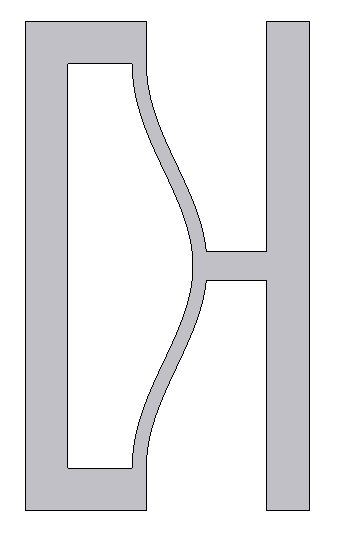
\includegraphics[width=0.3\textwidth]{FIGS/cell.png}
    \caption{Curved-beam metamaterial unit cell considered in this work. The
    geometry is inspired by negative-stiffness designs based on cosine-shaped
    curved beams undergoing snap-through instabilities.}
    \label{fig:cell_geometry}
\end{figure}

\begin{figure}[H]
    \centering
    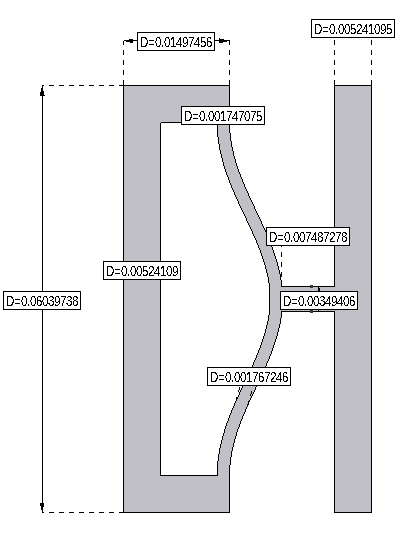
\includegraphics[width=0.3\textwidth]{FIGS/dimensions.png}
    \caption{Geometrical definition of the curved-beam metamaterial unit cell.
    The characteristic dimensions of the structure are indicated in the figure.
    These include the overall height and width of the cell, the thickness of the
    lateral walls, the width of the transverse connector, and the geometric
    parameters defining the curved ligament. The values reported correspond to
    the reference configuration used in the numerical simulations (units in meters).}
    \label{fig:dimensions}
\end{figure}

\subsubsection{Material properties}

 \PROMPT{Regarding the material properties, these are defined in   /home/joaquin/Desktop/CURRENT_TASKS/MATLAB_CODES/TESTING_PROBLEMS_FEHROM/115_PAPER_MAW_ECM/01_METATcellHOM_2var/ElasticMaterialDATA_NH.m   (put this into a \MATLAB{}) comment.  E = 1628     MPa, Young's modulus
nu = 0.4 Poisson's coefficient}


\subsubsection{Constitutive model}

The base material of the metamaterial cell is modeled as an isotropic
compressible Neo--Hookean solid. The elastic parameters are taken as
$E = 1628~\mathrm{MPa}$ and $\nu = 0.4$, where $E$ is Young's modulus and
$\nu$ is Poisson's ratio (these values correspond to a high-impact ABS material.


\MATLAB{The material parameters are defined in
\href{/home/joaquin/Desktop/CURRENT_TASKS/MATLAB_CODES/TESTING_PROBLEMS_FEHROM/115_PAPER_MAW_ECM/01_METATcellHOM_2var/ElasticMaterialDATA_NH.m}{ElasticMaterialDATA\_NH.m}.
The constitutive model is selected through
\texttt{DATA.TYPE\_CONSTITUTIVE\_MODEL\_ALL = 'NeoHookean'}.
The parameters used are \texttt{E = 1628} MPa and \texttt{nu = 0.4}.}


\subsection{Finite element discretization}

The unit cell is discretized using standard two-dimensional quadrilateral
finite elements with linear interpolation (four-node elements). A characteristic
element size of the order of $10^{-4}$ m is employed, resulting in a mesh
comprising 1315 elements and 1602 nodes.

The mesh is constructed to ensure compatibility along opposite boundaries of
the unit cell. In particular, a structured nodal distribution is imposed along
the boundary lines so that nodes on opposing sides are aligned and can be
directly paired. This requirement stems from the imposition of periodic boundary
conditions in the homogenization framework.

\begin{figure}[H]
    \centering
    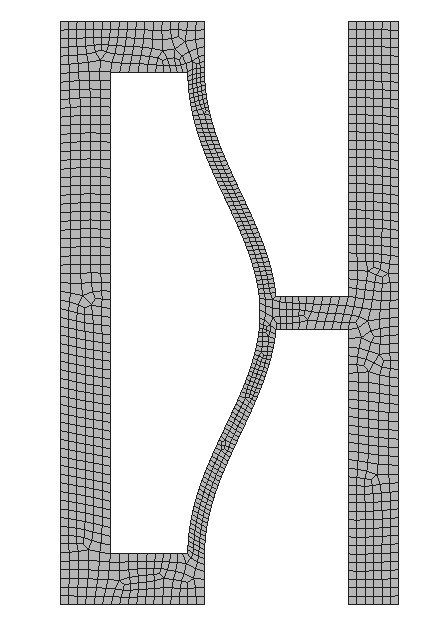
\includegraphics[width=0.35\textwidth]{FIGS/mesh.png}
    \caption{Finite element discretization of the metamaterial unit cell.}
    \label{fig:mesh}
\end{figure}


\subsection{Boundary conditions}

\PROMPT{\input{Prompt_bc.tex}}



Since a first-order computational homogenization setting is adopted, the
macroscopic input is the deformation gradient, denoted by $\Fmacro$. In plane
strain, this tensor can be expressed as
\[
\Fmacro
=
\begin{bmatrix}
F_x & F_{xy} \\
F_{yx} & F_y
\end{bmatrix}.
\]
In general, this representation involves four independent components. However,
part of this information corresponds to rigid-body rotations, which are not
relevant for the present objective. In order to exclude rotational effects, we
restrict attention to symmetric deformations by enforcing $F_{xy} = F_{yx}$.
As a result, only the deformational part of $\Fmacro$ is retained, reducing the
parametric space to three independent variables.

In this example, we do not explore the complete three-dimensional deformation
space. This choice is twofold. First, the purpose of the example is to analyze
the adaptive-weight ECM construction, not to address the general problem of
high-dimensional regression. Second, for the present cell, the dominant
mechanism is activated by deformation along the weak direction of the
microstructure, namely the horizontal \(x\)-direction, along which the curved
beams undergo snap-through-like deformation.

Accordingly, the prescribed macroscopic deformation is restricted to two
components: stretching/compression in the \(x\)-direction and in-plane shear.
The former is the principal loading mode for which the negative-stiffness
mechanism is designed. The latter is included because, although these devices
are primarily conceived to operate under compression or tension, shear
components may naturally arise from misalignment or non-ideal loading
conditions. In particular, shear perturbations may break the symmetry of the
response and induce non-synchronous buckling of the curved beams, an effect that
will be illustrated later.



\PROMPT{Now let us describe how to explore the parameteric space. We choose a structured grid of sampling points of $F_x^{macro}$ and $F_{xy}^{macro}$, that is, we have to specify the ``corners'' of the parametric space (please, put this more elegantly).  So, from the training point of view, we have to determine finite element states by solving the equilibrium of the unit cell for varying values of these two parameters (with $F_y = 1$). Actually, now that I think, it is better to use the gradient of displacements.  Let us elaborate this a little bit further by inspecting how it is done in the code (everything related to the code should be put into a \\MATLAB{} note, because I will hide it when writing the paper. Be that as it may, in the case that we are going to show later, the running script is /home/joaquin/Desktop/CURRENT_TASKS/MATLAB_CODES/TESTING_PROBLEMS_FEHROM/115_PAPER_MAW_ECM/01_METATcellHOM_2var/Run_HOMOG_2p.m.   The input data file is /home/joaquin/Desktop/CURRENT_TASKS/MATLAB_CODES/TESTING_PROBLEMS_FEHROM/115_PAPER_MAW_ECM/01_METATcellHOM_2var/DATAINPUTS/Data_M3.m, and then, inside:  /home/joaquin/Desktop/CURRENT_TASKS/MATLAB_CODES/TESTING_PROBLEMS_FEHROM/115_PAPER_MAW_ECM/01_METATcellHOM_2var/BC2v_M.m    ....There, there are two parameters DATAOUT.INPp.ParameterDomain_F_11 = [-0.42,0.42], DATAOUT.INPp.ParameterDomain_F_12 = [-0.05,0.05];DATAOUT.INPp.nsteps_F11 = 230;
DATAOUT.INPp.nsteps_F_12 = 20 ;  and /home/joaquin/Desktop/CURRENT_TASKS/MATLAB_CODES/TESTING_PROBLEMS_FEHROM/115_PAPER_MAW_ECM/01_METATcellHOM_2var/DetermineTrajectories_cg.m   and /home/joaquin/Desktop/CURRENT_TASKS/MATLAB_CODES/TESTING_PROBLEMS_FEHROM/115_PAPER_MAW_ECM/01_METATcellHOM_2var/buildGridTrajAndLabels.m. REad this and wait for my instructions

 )}

\subsection{Sampling of the macroscopic parameter space}

The training set is generated by sampling a two-dimensional subspace of the
macroscopic deformation space. Rather than working directly with the deformation
gradient, we prescribe the macroscopic displacement gradient
\[
\bm{G}^{\mathrm{macro}} = \Fmacro - \bm{I}.
\]
In the present example, only two components are varied:
\[
G^{\mathrm{macro}}_x
\quad \text{and} \quad
G^{\mathrm{macro}}_{xy},
\]
while the transverse component is kept fixed, \(G^{\mathrm{macro}}_y=0\). The
imposed macroscopic displacement gradient therefore has the form
\[
\bm{G}^{\mathrm{macro}}
=
\begin{bmatrix}
G^{\mathrm{macro}}_x & G^{\mathrm{macro}}_{xy} \\
G^{\mathrm{macro}}_{xy} & 0
\end{bmatrix},
\qquad
\Fmacro = \bm{I}+\bm{G}^{\mathrm{macro}} .
\]
The condition \(G^{\mathrm{macro}}_{xy}=G^{\mathrm{macro}}_{yx}\) removes the
rotational component and restricts the sampling to purely deformational states.

The sampled domain is defined by prescribing the lower and upper bounds of these
two parameters. In the reference case considered here, the compression/stretching
component along the soft direction of the cell is varied in the interval
\[
G^{\mathrm{macro}}_x \in [-0.42,\,0.42],
\]
whereas the shear component is varied in
\[
G^{\mathrm{macro}}_{xy} \in [-0.05,\,0.05].
\]
A structured grid is then introduced over this rectangular parameter domain, with
230 sampling values in the \(G^{\mathrm{macro}}_x\)-direction and 20 sampling
values in the \(G^{\mathrm{macro}}_{xy}\)-direction.

Although the final dataset is interpreted as a structured grid in parameter
space, the finite element simulations are not generated as independent isolated
points. Instead, the grid is traversed through two continuous zig-zag loading
trajectories. The first trajectory starts from the origin and sweeps the region
with non-negative shear; the second trajectory also starts from the origin and
sweeps the region with non-positive shear. The origin is therefore shared by
both paths but is retained only once in the final snapshot ordering.

This construction has two advantages. First, the finite element states are
generated along continuous loading paths, which is convenient for nonlinear
quasi-static simulations. Second, every snapshot is assigned a unique position in
the structured parameter grid. This makes it possible to reshape reduced
quantities, such as master coordinates, slave coordinates, or adaptive weights,
back onto the two-dimensional parameter domain for visualization and regression.

\MATLAB{The numerical experiment is launched from
\href{/home/joaquin/Desktop/CURRENT_TASKS/MATLAB_CODES/TESTING_PROBLEMS_FEHROM/115_PAPER_MAW_ECM/01_METATcellHOM_2var/Run_HOMOG_2p.m}{Run\_HOMOG\_2p.m}.
The input data are defined in
\href{/home/joaquin/Desktop/CURRENT_TASKS/MATLAB_CODES/TESTING_PROBLEMS_FEHROM/115_PAPER_MAW_ECM/01_METATcellHOM_2var/DATAINPUTS/Data_M3.m}{DATAINPUTS/Data\_M3.m}.
The boundary-condition sampling is specified in
\href{/home/joaquin/Desktop/CURRENT_TASKS/MATLAB_CODES/TESTING_PROBLEMS_FEHROM/115_PAPER_MAW_ECM/01_METATcellHOM_2var/BC2v_M.m}{BC2v\_M.m},
where the parameter bounds are
\texttt{ParameterDomain\_F\_11 = [-0.42,0.42]},
\texttt{ParameterDomain\_F\_12 = [-0.05,0.05]},
with \texttt{nsteps\_F11 = 230} and \texttt{nsteps\_F\_12 = 20}. The trajectories
and the structured snapshot ordering are generated by
\href{/home/joaquin/Desktop/CURRENT_TASKS/MATLAB_CODES/TESTING_PROBLEMS_FEHROM/115_PAPER_MAW_ECM/01_METATcellHOM_2var/DetermineTrajectories_cg.m}{DetermineTrajectories\_cg.m},
which calls
\href{/home/joaquin/Desktop/CURRENT_TASKS/MATLAB_CODES/TESTING_PROBLEMS_FEHROM/115_PAPER_MAW_ECM/01_METATcellHOM_2var/buildGridTrajAndLabels.m}{buildGridTrajAndLabels.m}.}


The sampled macroscopic parameter domain is shown in
Fig.~\ref{fig:param_space}. The two varying input quantities are the components
of the macroscopic displacement gradient, namely
$G^{\mathrm{macro}}_x$ and $G^{\mathrm{macro}}_{xy}$. The former controls the
horizontal stretching/compression of the unit cell, while the latter introduces
a symmetric shear perturbation. The domain is intentionally restricted to a
two-dimensional rectangle in order to keep the regression problem simple and to
allow a direct graphical inspection of the adaptive weights.

The lower bound $G^{\mathrm{macro}}_x=-0.42$ corresponds to a highly compressed
configuration in which the curved ligaments approach the opposite wall, without
reaching self-contact in the reference simulations. The corner configurations
shown in the figure illustrate the extreme combinations of axial
stretching/compression and positive/negative shear. The two colored paths
represent the loading trajectories used to traverse the grid of sampling
points.

\begin{figure}[H]
    \centering
    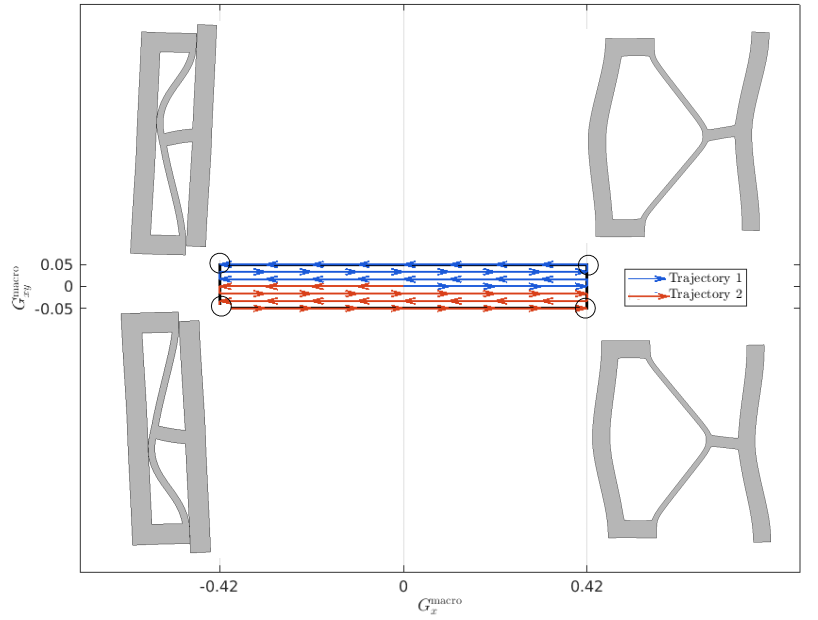
\includegraphics[width=1\textwidth]{FIGS/param_space.png}
    \caption{Sampled two-dimensional macroscopic parameter domain. The varying
    input quantities are the components of the macroscopic displacement
    gradient, $G^{\mathrm{macro}}_x$ and $G^{\mathrm{macro}}_{xy}$, while the
    transverse component is kept fixed. The rectangular domain is bounded by
    the minimum and maximum values used in the training set. The deformed
    configurations at the four corners illustrate the extreme combinations of
    horizontal compression/stretching and positive/negative shear. The two
    colored curves indicate the loading trajectories used to traverse the
    parameter grid.}
    \label{fig:param_space}
\end{figure}



\section{Finite element formulation of the unit-cell problem}

\PROMPT{\input{Prompt_bc2}}




%\input{Micro_v1disp}


\subsection{Microscopic equilibrium problem}
\label{sec:mequilibrium}
For each prescribed macroscopic displacement gradient $\Gmacro$, the state of
the unit cell is determined by the microscopic displacement field, represented
after finite element discretization by the nodal vector $\dvec$. We work
directly with the \emph{total displacement field}, without separating
fluctuations.

Under periodic boundary conditions, the displacement vector admits the decomposition
\begin{equation}
\label{eq:dvecreconstruction}
 \dvec = \Alift \dred + \Umacro \muvec .
\end{equation}
Here, $\dred$ collects the independent unknowns of the problem, namely the
interior degrees of freedom together with a subset of boundary\footnote{Here and in what follows  ``boundary'' refers to the external boundary
$\partial\Omega_0$ of the reference unit cell, i.e., the interface with adjacent
cells in the periodic homogenization setting.} degrees of
freedom chosen as masters (in the present case, nodes on the left boundary and
on the bottom edge, excluding corner nodes). The matrix $\Alift$ is the
constraint-lifting operator associated with the periodic boundary conditions:
it maps the independent unknowns $\dred$ into the full nodal displacement space
and contains the master--slave coupling imposed by periodicity. The remaining
boundary nodes (top and right edges, as well as corners) are treated
as slave degrees of freedom.

The matrix $\Umacro$ encodes the affine macroscopic deformation. Its rows are
zero for all independent degrees of freedom (interior and master nodes), while
nonzero entries appear only for slave boundary nodes and   corner
nodes, where the displacement is prescribed through the macroscopic gradient.

The vector $\muvec$ parameterizes the imposed macroscopic deformation; in the
present setting, $\muvec = (G_x^{\mathrm{macro}},
G_{xy}^{\mathrm{macro}})^T$, with $G_y^{\mathrm{macro}}=0$.

For a node $\bm{X}=(X,Y)^T$ belonging to a slave boundary, the affine macroscopic contribution is defined in the reference
configuration as $\bar{\bm{u}}(\bm{X})=\Gmacro \bm{X}$, which in the present
case yields $\bar{\bm{u}}(\bm{X})=(G_x^{\mathrm{macro}}X+G_{xy}^{\mathrm{macro}}Y,\,
G_{xy}^{\mathrm{macro}}X)^T$. This contribution is assembled into
$\Umacro\muvec$, acting only on constrained boundary degrees of freedom.


The microscopic equilibrium is expressed through the finite element nodal residual, which in the present case (with no nodal external forces) reduces to  the nodal vector of internal force vector:
\begin{equation}
 \Fint(\dvec)=\int_{\Omega_0}\Bmat^T(\bm{X})\,\PKone(\dvec,\bm{X})\,d\Omega_0.
\end{equation}
\noindent  After finite element discretization and Gauss quadrature, the above  adopts the expression
\begin{equation}
\label{eq:33333}
    \Fint(\dvec)
    =
    \sum_{e=1}^{n_{\mathrm{el}}}
   \Le^T
    \left(
    \sum_{g=1}^{n_{\mathrm{gp}}^{(e)}}
    \Bmat_{e,g}^T \, \PKone_{e,g} \, w_{e,g}
    \right),
\end{equation}
where $\Le$ is the standard Boolean assembly operator mapping
element degrees of freedom to global ones, $\Bmat_{e,g}$ is the element-level
displacement-gradient operator (Voigt notation),   $\PKone_{e,g}$ is the
first Piola--Kirchhoff stress and $w_{e,g}$ denotes the physical quadrature weight associated with Gauss
point $g$ of element $e$, including both the parent-domain Gauss weight and the
Jacobian determinant of the isoparametric mapping.

The above expression corresponds to the standard finite element nodal internal
force vector. However, the equilibrium problem is posed in the space of
independent degrees of freedom through the lifting operator $\Alift$, in
accordance with the principle of virtual work. This leads to the constrained
equilibrium condition $\Alift^T \Fint(\dvec) = \bm{0}$. Using~\eqref{eq:33333},
and reindexing the element/Gauss-point pairs $(e,g)$ by a single global index,
this can be written as
\begin{equation}
\label{eq:013}
      \sum_{g=1}^{\ngp}
    \rFE{g}(\dvec)\, \wFEg{g}
    =
    \bm{0},
\end{equation}
where
\begin{equation}
    \rFE{g}(\dvec)
    :=
    \Alift^T \Le^T \Bmat_{e,g}^T \PKone_{e,g}(\dvec)
    \in \mathbb{R}^{\nL}
\end{equation}
denotes the   internal force contribution (per unit volume) associated with the global
Gauss point $g$, and $\wFEg{g} >0$ is the corresponding
quadrature weight (here, the superscript ``FE'' emphasizes that $\wFEg{g}$ denotes the quadrature
weights of the underlying finite element discretization, to be distinguished
later from the cubature weights used in hyperreduction.).  Eq. \ref{eq:013} constitutes the full-order nonlinear problem used to generate the snapshot
data; subsequent model reduction acts on $\dred$, i.e., on the independent
microscopic degrees of freedom after enforcement of periodicity and affine
lifting.
\begin{remark}[Gauss-point vs element-based representation]
An equivalent expression can be written at the element level by regrouping the
Gauss-point contributions within each element. In that case, the summation runs
over elements, the weights are replaced by the element measure, and the
corresponding contribution is defined as the element-averaged internal force.
Equivalently, one may incorporate the quadrature weights into the definition of
$\rFE{g}$, so that the equilibrium equation is expressed as a sum  of (sparse) elemental internal force contributions.
\end{remark}




\MATLAB{The general infrastructure for imposing time-dependent Dirichlet and
periodic boundary conditions is implemented in
\href{/home/joaquin/Desktop/CURRENT_TASKS/MATLAB_CODES/BACKUPS_FE_HROM/CODE/LARGE_STRAINS/InputDataFunctions/DirichletCONDtime_GENERAL.m}{DirichletCONDtime\_GENERAL.m}.
In the present case, periodic homogenization boundary conditions are imposed
through
\href{/home/joaquin/Desktop/CURRENT_TASKS/MATLAB_CODES/FE_HROM/LARGE_STRAINS/InputDataFunctions/DirichletCONDtime_PeriodHomogQ4samALL.m}{DirichletCONDtime\_PeriodHomogQ4samALL.m},
which calls
\href{/home/joaquin/Desktop/CURRENT_TASKS/MATLAB_CODES/FE_HROM/LARGE_STRAINS/InputDataFunctions/PeriodicQ4_homogCAN.m}{PeriodicQ4\_homogCAN.m}.
For comparison, the homogeneous affine Dirichlet version is documented in
\href{/home/joaquin/Desktop/CURRENT_TASKS/MATLAB_CODES/FE_HROM/LARGE_STRAINS/InputDataFunctions/DirichletCONDtime_homogZEROall.m}{DirichletCONDtime\_homogZEROall.m}.}

\subsection{Homogeneized stresses}
 \label{subsec:homogenized_PK1}


\PROMPT{\input{ChangingCHAT_01}}


\PROMPT{\input{PR_HOM_stress}}

Although the reduced model reconstructs the microscopic displacement field, the
primary quantity of interest in first-order computational homogenization is the
homogenized first Piola--Kirchhoff stress. This quantity can be obtained either
as the volume average of the microscopic stress field or, equivalently, from the
boundary reactions \cite{miehe1999computational}. Using the volume-average representation, we write:
\begin{equation}
\label{eq:macro3}
    \PKmacro
    =
    \frac{1}{|\Omega_0|}
    \int_{\Omega_0} \PKone(\dvec,\bm{X}) \, d\Omega_0
    \;=\;
    \frac{1}{|\Omega_0|}
    \sum_{g=1}^{\ngp}
    \PKone_g(\dvec)\,\wFEg{g}.
\end{equation}

\MATLAB{In the finite element post-processing, the reaction-based homogenized stresses
are evaluated in
\href{/home/joaquin/Desktop/CURRENT_TASKS/MATLAB_CODES/FE_HROM/LARGE_STRAINS/NonLinearManifolds/CHECK_consistency_non_gen3Rg.m}{CHECK\_consistency\_non\_gen3Rg.m}.
When \texttt{ComputeHomogeneizedStresses = 1}, the code collects all boundary nodes,
builds the matrix \texttt{X\_homog\_stress} from their reference coordinates, computes
\texttt{PK1stress\_homg = X\_homog\_stress*REACTIONS\_FE(DOFsBND,:)}, and normalizes
by \texttt{VOL = sum(OPERFE.wSTs)}.  }

\section{Standard hyperreduced-order model }
 \label{sec:standard_ROM}


\PROMPT{\input{Prompt_stdROM}}


\subsection{Linear reduced subspace}
\label{subsec:linear_reduced_subspace}

As a first compressed representation, we consider a standard projection-based ROM in which
the independent displacement vector $\dred$ is approximated in a linear reduced subspace,
\begin{equation}
    \dred \approx \PhiROM \qrom ,
    \label{eq:standard_ROM_expansion}
\end{equation}
where $\PhiROM\in\mathbb{R}^{\nL\times\rROM}$ contains precomputed displacement modes,
$\qrom\in\mathbb{R}^{\rROM}$ is the vector of reduced coordinates, $\nL$ is the number of
independent degrees of freedom after imposing periodic constraints, and $\rROM$ is the
dimension of the reduced space. In the present problem, $\nL=3018$.

The basis $\PhiROM$ is obtained from the snapshot matrix
\begin{equation}
\label{eq:Dmatrix}
    \Dsnap =
    \begin{bmatrix}
    \dred(\mu_1) & \dred(\mu_2) & \cdots & \dred(\mu_{\nsnap})
    \end{bmatrix}
    \in\mathbb{R}^{\nL\times\nsnap},
\end{equation}
where $\nsnap$ denotes the number of training snapshots. Since the parameter domain is
sampled on a structured two-dimensional grid, the total number of snapshots is
$\nsnap=4852$, stored in two trajectory blocks of size $3018\times2426$ after restriction to
the independent degrees of freedom.

The modal basis is computed by a truncated singular value decomposition of $\Dsnap$.
In practice, this operation may be performed by any equivalent memory-aware SVD strategy,
including block, partitioned, or randomized variants. In the present implementation we use the
sequential randomized SVD machinery described in \cite{hernandez2024cecm}. The truncation
criterion is based on the relative Frobenius norm of the discarded singular values.

\MATLAB{The standard ROM basis is generated by running
\href{/home/joaquin/Desktop/CURRENT_TASKS/MATLAB_CODES/TESTING_PROBLEMS_FEHROM/115_PAPER_MAW_ECM/01_METATcellHOM_2var/Run_HOMOG_2p.m}{Run\_HOMOG\_2p.m}
with input file
\href{/home/joaquin/Desktop/CURRENT_TASKS/MATLAB_CODES/TESTING_PROBLEMS_FEHROM/115_PAPER_MAW_ECM/01_METATcellHOM_2var/DATAINPUTS/Data_M3std.m}{DATAINPUTS/Data\_M3std.m},
where \texttt{DATAoffline.Hyperreduction\_METHOD\_projection = 'STANDARD'} and
\texttt{DATA\_interp.METHOD\_SELECT\_REFERENCE\_MODE = 'STANDARD\_ROM'}.
The offline construction is performed in
\href{/home/joaquin/Desktop/CURRENT_TASKS/MATLAB_CODES/FE_HROM/LARGE_STRAINS/NonLinearManifolds/Determine_qinf_qsup_STDROM.m}{Determine\_qinf\_qsup\_STDROM.m}.
The snapshot blocks are first restricted to \texttt{DOFl}; in the present case
\texttt{SNAPdisp = \{3018 x 2426, 3018 x 2426\}}. With
\texttt{DATAoffline.errorDISP = 1e-6}, the call
\texttt{[Phi,S,V] = SRSVD(SNAPdisp,TOL\_BLOCK,DATAsvd)} returns
\texttt{size(Phi,2) = 52}.}

\subsection{Compressibility of the displacement snapshots}
\label{subsec:standard_ROM_compressibility}

Figure~\ref{fig:svd_truncation_error} shows the relative Frobenius truncation error obtained
from the singular values of $\Dsnap$. The decay is regular, but not sufficiently steep to regard
the solution set as strongly compressible by a very low-dimensional linear subspace.

\begin{figure}[H]
    \centering
    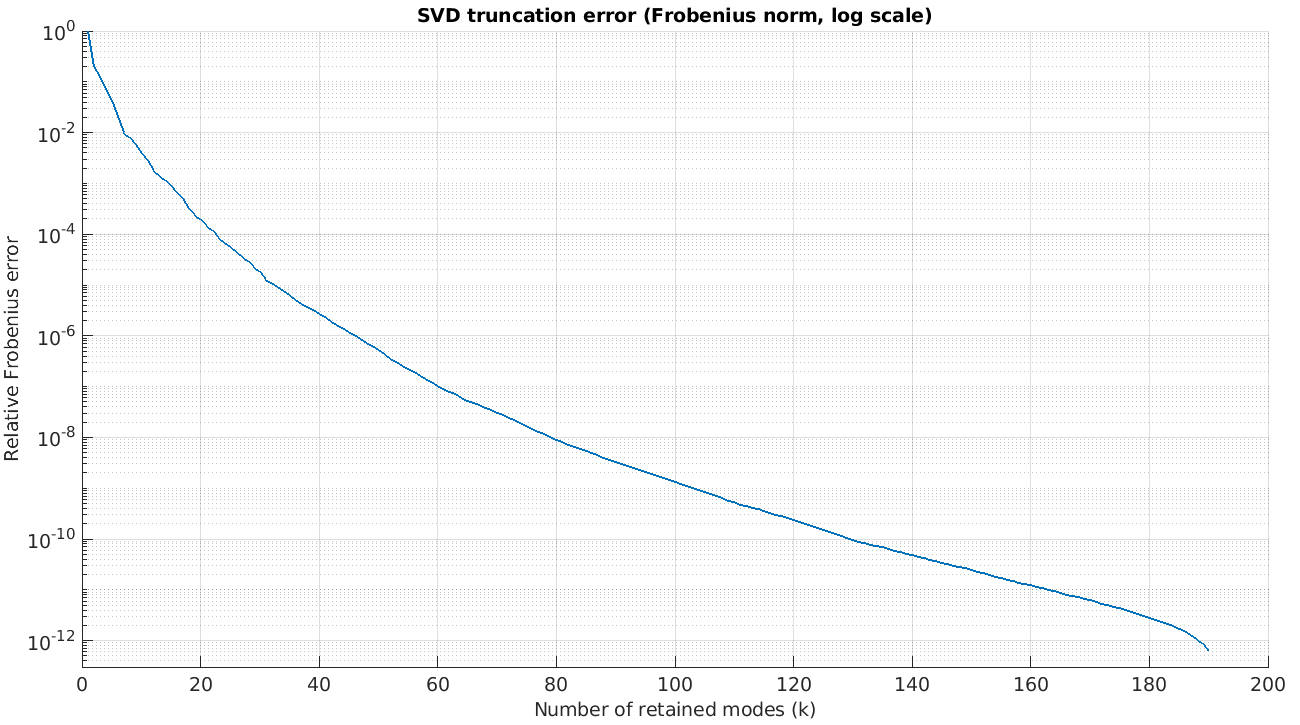
\includegraphics[width=0.78\textwidth]{FIGS/Graph_Singular_Values.png}
    \caption{Relative Frobenius truncation error associated with the singular values of the
    displacement snapshot matrix $\Dsnap$.}
    \label{fig:svd_truncation_error}
\end{figure}

% Indeed, even if we have only two macroscopic variables,  a moderate level of accuracy already requires a relatively large number of modes. For instance, for a relative Frobenius truncation error of order $10^{-6}$  we need  $\rROM=52$  for the problem under consideration (for illustration purposes, some of these modes are shown in Figure ).  Even a less stringent accuracy level requires on the order of $40$ modes.


Indeed, even if we have only two macroscopic variables, a moderate level of
accuracy already requires a relatively large number of modes. For instance, for
a relative Frobenius truncation error of order $10^{-6}$ we need $\rROM=52$ for
the problem under consideration (for illustration purposes, some of these modes
are shown in Figure~\ref{fig:...}). Reducing the tolerance to $10^{-5}$ and
$10^{-4}$ decreases the number of retained modes to $\rROM=37$ and
$\rROM=25$, respectively.

The implications of these truncation levels are not immediately apparent from
the a priori SVD error alone. A more meaningful assessment is obtained by
examining the a posteriori errors in the reconstructed fields and derived
quantities, such as the homogenized stresses. This analysis is deferred to
Section~\ref{subsec:standard_HROM_accuracy}, where the impact of the reduced
basis dimension on both displacement and stress accuracy is quantified.


\begin{remark}
This behavior is a manifestation of the classical Kolmogorov $n$-width limitation of linear
reduced spaces: the solution manifold may be low-dimensional in terms of its parametrization
but poorly aligned with any low-dimensional affine or linear subspace. The situation is
expected to deteriorate further when additional macroscopic deformation components are
varied. In particular, including the transverse strain component would increase the
complexity of the displacement manifold, and this effect would be even more pronounced
in three-dimensional settings, where up to six independent strain components may act as
inputs. Consequently, the standard ROM provides a useful baseline, but it is not the most appropriate
reduced representation for the present problem.
\end{remark}


%
% \PROMPT{Create a Figure with subfigures FIGS/Modes_1.png, FIGS/Modes_2.png,  FIGS/Modes_3.png,   FIGS/Modes_20.png,  FIGS/Modes_40.png, FIGS/Modes_52.png. These contain the deformed shapes corresponding to displacement modes 1, 2, 3, 20, 40 and 52. Say in the caption that although modes are only defined at the independet nodal DOFs, they have been extended to the remaining DOFs for visualization purposes (try to explain this elegantly, but very short and compact). Say also that the first modes (1,2,3) capture long range effects (I don't know how to say it, I want to say that it captures macroscopic displacement, more notiable); in contrast 20, 40 and 52 are more related with changes in the two curved beams (capture buckling effects....) }


\begin{figure}[H]
\centering
\begin{subfigure}{0.32\textwidth}
    \centering
    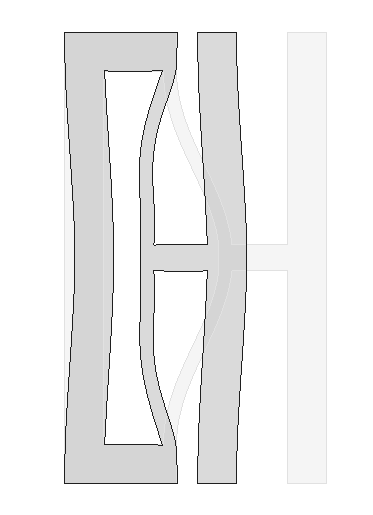
\includegraphics[width=\textwidth]{FIGS/Modes_1.png}
    \caption{Mode 1 ($\PhiROM_{1}$)}
\end{subfigure}
\begin{subfigure}{0.32\textwidth}
    \centering
    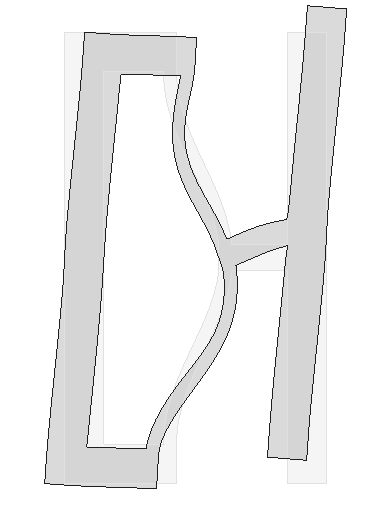
\includegraphics[width=\textwidth]{FIGS/Modes_2.png}
    \caption{Mode 2 ($\PhiROM_{2}$)}
\end{subfigure}
\begin{subfigure}{0.32\textwidth}
    \centering
    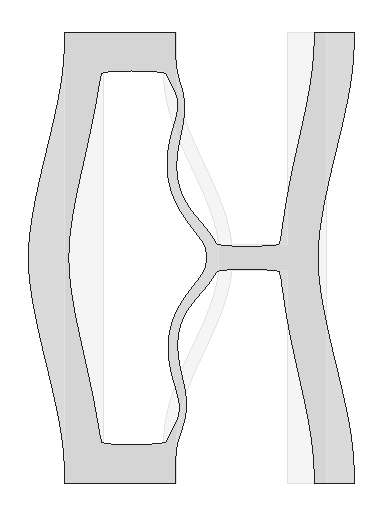
\includegraphics[width=\textwidth]{FIGS/Modes_3.png}
    \caption{Mode 3 ($\PhiROM_{3}$)}
\end{subfigure}

\vspace{0.5em}

\begin{subfigure}{0.32\textwidth}
    \centering
    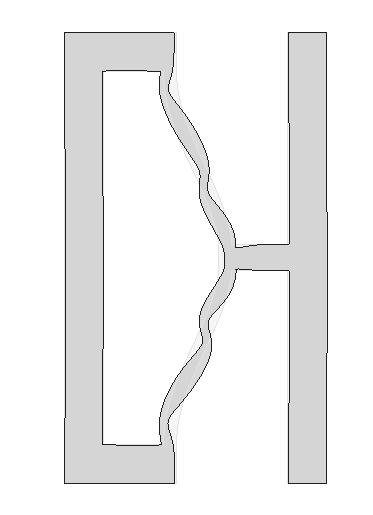
\includegraphics[width=\textwidth]{FIGS/Modes_20.png}
    \caption{Mode 20 ($\PhiROM_{20}$)}
\end{subfigure}
\begin{subfigure}{0.32\textwidth}
    \centering
    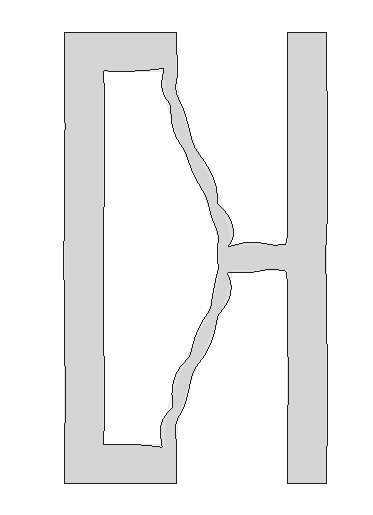
\includegraphics[width=\textwidth]{FIGS/Modes_40.png}
    \caption{Mode 40 ($\PhiROM_{40}$)}
\end{subfigure}
\begin{subfigure}{0.32\textwidth}
    \centering
    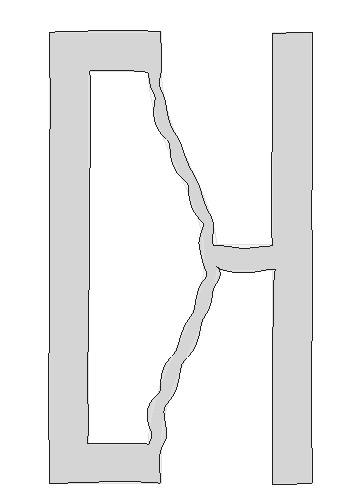
\includegraphics[width=\textwidth]{FIGS/Modes_52.png}
    \caption{Mode 52 ($\PhiROM_{52}$)}
\end{subfigure}

\caption{Deformed shapes associated with selected modes of the   ROM basis. Although the modes are defined only on the independent degrees of freedom, they are extended to the full displacement field for visualization purposes through the constraint-lifting operator. The first modes (1--3) capture global deformation patterns associated with the macroscopic response, whereas higher modes (20, 40, 52) are increasingly localized and mainly describe deformation and buckling mechanisms in the curved ligaments.}
\label{fig:ROM_modes}
\end{figure}


\subsection{Equilibrium equation in the reduced space and hyperreduction}
 \label{subsec:Galerkin_hyperreduction}

\PROMPT{\input{Prompt_HROM}}
%\input{HROM_v1}
\PROMPT{\input{Prompt_HROM1}}



We take as starting point the constrained equilibrium equation written in
Gauss-point form, cf.~\eqref{eq:013}. Introducing the linear ROM approximation
and restricting the virtual displacements to the same space, the Galerkin form
of the principle of virtual work yields
\begin{equation}
\label{eq:ROM_equilibrium_FE_weights}
      \sum_{g=1}^{\ngp}
    \rPhi{g}(\qrom;\muvec)\,\wFEg{g}
    =
    \bm{0},
\end{equation}
where
\begin{equation}
\label{eq:rPhi_definition}
    \rPhi{g}(\qrom;\muvec)
    :=
    \PhiROM^T
    \rFE{g}\!     \in \mathbb{R}^{\rROM}.
\end{equation}

Equation~\eqref{eq:ROM_equilibrium_FE_weights} defines a system of $\rROM$
nonlinear equations for the reduced coordinates $\qrom$. It is important to note
that, although the equilibrium equation has been modified through the projection
onto the reduced space (as reflected in $\rPhi{g}$), the integration rule remains
unchanged: the summation still runs over all $\ngp$ Gauss points and employs the
original FE weights $\wFEg{g}$.


\subsubsection{Hyperreduction (equilibrium)}

This observation provides the natural entry point for hyperreduction. From a
quadrature (or, more precisely, cubature) perspective, the goal is to construct a
reduced integration rule tailored to the reduced integrands $\rPhi{g}$. This
amounts to selecting a subset of Gauss points
\[
    \Zred \subset \{1,\ldots,\ngp\},
\]
together with associated positive weights $\wPhig{g}$, such that the equilibrium
equation can be approximated as
\begin{equation}
\label{eq:013aaa}
      \sum_{g\in \Zred}
    \rPhi{g}(\qrom;\muvec)\,\wPhig{g}
    =
    \bm{0}.
\end{equation}
The construction of $\Zred$ and $\wPhig{g}$ is therefore a discrete selection
problem, in which only a small subset of the original Gauss points is retained.


For a single training state, characterized by $\muvec_j$ and by the corresponding
ROM coordinates $\qrom_j$, the projected equilibrium equation can be written as
\begin{equation}
    \aforce(\qrom_j;\muvec_j)^T \wFE = \bm{0},
    \label{eq:single_state_reduced_integrand_matrix}
\end{equation}
where
\begin{equation}
    \aforce(\qrom_j;\muvec_j)
    =
    \begin{bmatrix}
        \rPhi{1}(\qrom_j;\muvec_j)^T\\
        \rPhi{2}(\qrom_j;\muvec_j)^T\\
        \vdots\\
        \rPhi{\ngp}(\qrom_j;\muvec_j)^T
    \end{bmatrix}
    \in \mathbb{R}^{\ngp\times\rROM}.
    \label{eq:single_state_aforce}
\end{equation}
and
\begin{equation}
    \wFE =
    \begin{bmatrix}
        \wFEg{1}\\
        \wFEg{2}\\
        \vdots\\
        \wFEg{\ngp}
    \end{bmatrix}
    \in \mathbb{R}^{\ngp},
\end{equation}
Thus, each column of $\aforce(\qrom_j;\muvec_j)$ represents one scalar
reduced-integrand field over the Gauss points of the mesh.

Collecting these matrices for all training states gives the global snapshot
matrix of reduced internal-force densities,
\begin{equation}
\label{eq:aforce_orig}
    \Aforce
    =
    \begin{bmatrix}
        \aforce(\qrom_1;\muvec_1) &
        \aforce(\qrom_2;\muvec_2) &
        \cdots &
        \aforce(\qrom_{\nsnap};\muvec_{\nsnap})
    \end{bmatrix}
    \in \mathbb{R}^{\ngp\times(\rROM\nsnap)}.
    \label{eq:Aforce_training_matrix}
\end{equation}
The columns of $\Aforce$ span the family of scalar fields that must be
integrated accurately by the new cubature rule. Accordingly, the goal is to
construct a basis matrix for the column space of $\Aforce$---this is the
underlying idea of the Empirical Cubature Method (ECM), see
\cite{hernandez2024cecm}.  To this end, a basis matrix
\begin{equation}
    \Ucub \in \mathbb{R}^{\ngp\times n_U},
    \qquad
    \operatorname{Range}(\Ucub) \approx \operatorname{Range}(\Aforce),
\end{equation}
is computed, typically via a truncated singular value decomposition of
$\Aforce$, so that $n_U \ll \rROM\nsnap$ after truncation. A natural choice is
to employ a weighted SVD, using the norm induced by the FE weights. The
cubature rule is then constructed so as to integrate exactly the columns of
$\Ucub$, rather than those of the full matrix\footnote{In contrast, related hyperreduction techniques such as the Energy-Conserving
Sampling and Weighting (ECSW) method and its variants
\cite{farhat2014dimensional,farhat2015structure} operate directly on the sampled
matrix (or on a subsampled set of its columns), without explicitly constructing
a reduced basis for the integrand space. The ECM strategy adopted here separates
these two steps: first identifying a low-dimensional space of relevant
integrands, and subsequently constructing a cubature rule tailored to that
space. In this framework, the approximation error in the integration is
introduced at the stage of basis truncation (e.g., via SVD), while the cubature
rule is designed to integrate exactly the retained basis functions.} $\Aforce$.

Following the ECM construction \cite{hernandez2024cecm}, the cubature rule is
obtained by solving a sparse selection problem. In the present discrete setting,
this can be formulated as
\begin{equation}
\label{eq:ECM_problem}
\begin{aligned}
    \min_{\wPhi} \quad & \|\wPhi\|_0 \\
    \text{s.t.} \quad & \Ucub^T \wPhi = \bFE, \\
                      & \wPhi \ge 0,
\end{aligned}
\end{equation}
where $\wPhi \in \mathbb{R}^{\ngp}$ is the vector of cubature weights, and
$\bFE \in \mathbb{R}^{n_U}$ contains the exact integrals of the columns of
$\Ucub$ computed with the FE quadrature rule, i.e.,
\begin{equation}
    \bFE = \Ucub^T \wFE.
\end{equation}
Problem~\eqref{eq:ECM_problem} seeks the sparsest vector of positive weights such
that the selected integration points reproduce exactly the integrals of the
basis functions. The support of $\wPhi$ defines the reduced set of Gauss points
$\Zred$, so that the cubature rule is obtained as a discrete subset of the
original FE integration points.


\PROMPT{\input{Prompt_HROM4}}

%\input{HROM_cont}
%\input{HROM_cont1}
%-\input{HROM_cont3}
\subsubsection{Remarks on the ECM formulation}
\label{subsec:remarks_ECM}

\begin{remark}[Well-posedness and inclusion of constants]
In the present setting, the vector of exact integrals $\bFE=\Ucub^T\wFE$ is zero
(or numerically close to zero), since the snapshots are extracted from
converged solutions of the nonlinear equilibrium problem, for which the residual
is driven to zero up to the tolerance of the Newton--Raphson procedure. As a
consequence, the optimization problem admits the trivial solution
$\wPhi=\bm{0}$.

To remove this degeneracy \cite{hernandez2017dimensional}, we impose the
additional normalization constraint that the cubature rule must exactly
reproduce the measure of the domain:
\begin{equation}
    \onevec^T \wPhi = |\Omega_0|,
\end{equation}
where $\onevec \in \mathbb{R}^{\ngp}$ denotes the all-ones vector.

This requirement can be enforced by appending the vector $\onevec$ to the basis
matrix $\Ucub$ (and augmenting $\bFE$ with the corresponding measure
$|\Omega_0|$). Alternatively, to preserve the orthogonality of $\Ucub$ (which is
desirable for the efficiency of the ECM algorithm), one may instead add only the
component of $\onevec$ that is orthogonal to the current column space of
$\Ucub$. Further details can be found in
\cite{hernandez2017dimensional,hernandez2024cecm}.
\end{remark}

\begin{remark}[Sparsity and connection with ECSW]
The $\ell_0$ formulation in~\eqref{eq:ECM_problem} is mainly conceptual and will
be useful later. The associated sparsification problem is NP-hard, and ECM does
not address it in this strict form. ECM instead relaxes the problem and simply seeks a
sparse nonnegative solution of the underdetermined system
$\Ucub^T\wPhi=\bFE$.  Inspired by the cubature strategy of An et al.~\cite{an2009optimizing},
  ECM  is built on a modification of the nonnegative least-squares
algorithm of Lawson and Hanson~\cite{lawson1995solving}. A distinctive feature of ECM is that the number of selected points  is known
a priori:   it coincides with the number of columns of
$\Ucub$, i.e., with the truncated rank of $\Aforce$. Thus, once the integrand
space has been compressed, the cubature problem reduces to selecting as many
integration points as basis functions, together with positive weights.

This aspect differs from related hyperreduction techniques such as the
Energy-Conserving Sampling and Weighting (ECSW) method\footnote{ECSW was originally formulated as a mesh (element) selection and weighting
strategy rather than as a cubature rule. However, when viewed through the
$\ell_0$-based formulation adopted here---actually borrowed from
\cite{farhat2014dimensional}---the two approaches become structurally equivalent
when the selected entities are finite elements, since in both cases the goal is
to approximate the integrals arising in the weak form using a reduced set of
contributions.}and its variants
\cite{farhat2014dimensional,farhat2015structure}, also based on the
Lawson--Hanson algorithm, which operate directly on the sampled matrix, or on a
subset of its columns. In ECM, basis extraction and cubature construction are
separated: the integration error is introduced at the stage of SVD truncation of
the integrand space, while the retained basis functions are integrated exactly.
By contrast, ECSW does not construct an explicit reduced basis for the
integrands; therefore, the integration error must be controlled directly at the
level of the sampling/weighting procedure, typically through a prescribed
tolerance on the residual of the approximation.
\end{remark}

%\subsubsection{Homogeneized stresses}


\PROMPT{\input{Prompt_HomogeneizedStress_1}}
%\input{HomogeneizedStress_1}
\subsection{Cubature rule for homogenized PK1 stresses}
\label{subsec:cubature_PK1_stresses}

We now consider the computation of the homogenized PK1 stress, previously
written in~\eqref{eq:macro3}. This quantity is an output functional, not an
equilibrium equation. Consequently, its hyperreduction can be addressed in two
different ways.

For a single training state $(\qrom_j,\muvec_j)$, define
\begin{equation}
    \aP(\qrom_j;\muvec_j)
    =
    \begin{bmatrix}
        \PKone_1(\qrom_j;\muvec_j)^T\\
        \PKone_2(\qrom_j;\muvec_j)^T\\
        \vdots\\
        \PKone_{\ngp}(\qrom_j;\muvec_j)^T
    \end{bmatrix}
    \in \mathbb{R}^{\ngp\times\nstress},
    \label{eq:aP_single_state}
\end{equation}
where $\nstress$ is the number of PK1 stress components retained in Voigt
notation. In the present two-dimensional large-strain setting, $\nstress=4$.
Each training state therefore adds $\nstress$ scalar integration constraints.

Collecting all training states gives the stress-output snapshot matrix
\begin{equation}
    \AP
    =
    \begin{bmatrix}
        \aP(\qrom_1;\muvec_1) &
        \aP(\qrom_2;\muvec_2) &
        \cdots &
        \aP(\qrom_{\nsnap};\muvec_{\nsnap})
    \end{bmatrix}
    \in \mathbb{R}^{\ngp\times(\nstress\nsnap)} .
    \label{eq:AP_training_matrix}
\end{equation}
This matrix plays for the homogenized stresses the same role that $\Aforce$
plays for the reduced internal-force densities.

A first possibility is to use a single cubature rule for both equilibrium and
output evaluation. In this case, the matrix used to construct the ECM basis is
enriched with the stress-output information contained in $\AP$, i.e., $\Ucub$ is
obtained as the left singular matrix of the concatenation\footnote{Since $\AP$ and $\Aforce$ correspond to different physical quantities
(with different units and scales), it is advisable to apply an appropriate
normalization prior to the SVD so as to balance their relative influence in the
resulting basis.  } of $\Aforce$ and $\AP$. The same selected
set $\Zred$ and weights $\wPhig{g}$ are then used both for the reduced residual
and for the homogenized PK1 stress:
\begin{equation}
\label{eq:simple1}
    \PKmacro
    \approx
    \frac{1}{|\Omega_0|}
    \sum_{g\in\Zred}
    \PKone_g(\qrom;\muvec)\,\wPhig{g}.
   % \label{eq:PKmacro_same_rule}
\end{equation}
This is the simplest online strategy, since only one set of Gauss points must be
stored, evaluated, and differentiated during the Newton iterations.

A second possibility is to construct a cubature rule specifically tailored to the
stress-output matrix $\AP$. This gives a possibly different set of points
$\ZP\subset\{1,\ldots,\ngp\}$ and weights $\wPg{g}$:
\begin{equation}
    \PKmacro
    \approx
    \frac{1}{|\Omega_0|}
    \sum_{g\in\ZP}
    \PKone_g(\qrom;\muvec)\,\wPg{g}.
    \label{eq:PKmacro_output_rule}
\end{equation}
This route may reduce the number of points required to integrate the output
alone, but it is less convenient computationally because two different point
sets must be tracked: one for the reduced residual and another one for the
homogenized stress. Although the stress output is needed only after convergence
of the nonlinear solve, the additional bookkeeping and stress evaluations may
still be undesirable.
If a separate output rule is used, it is advantageous to maximize its
intersection with the residual cubature set $\Zred$. For this purpose, one may
use the ECM variant proposed by the authors in \cite{bravo2024subspace}, which
accepts an initial candidate set. In the present context, $\Zred$ is taken as
such initial set; the algorithm first attempts to satisfy the stress
integration constraints using these points and enlarges the set only if
necessary, thereby maximizing the overlap between both cubature rules.


\subsection{Numerical assessment}
\label{sec:numassHROMstd}
\PROMPT{\input{NumAss_HROM_1}}



We now turn our attention to the numerical assessment of the performance of the ECM in the case discussed previously, in which the nodal displacement field requires $\rROM = 52$ modes to achieve a relative accuracy of $10^{-6}$. We adopt here the strategy in which a single cubature rule is used for both equilibrium and stress integration, cf. Eq.~\refeq{eq:simple1}. The underlying finite element discretization involves a total of $\ngp = \nel \,\ngpel = 5260$ Gauss integration points. For each instantiation of the input parameter, the corresponding contribution to $\left[\Aforce,\AP\right]$ consists of $\rROM + \nstress$ columns, accounting for the reduced equilibrium equations together with the stress-output contributions. Over the full training set of $\nsnap = 4852$ states, this leads to a total of $(\rROM + \nstress)\nsnap = (52+4)\times 4852 = 271712$ columns (recall that $\nstress = 4$ is the number of PK1 stress components retained in Voigt notation). It follows that the matrix whose column space must be approximated has size $5260 \times 271712$, that is, it is markedly wide, with roughly fifty times more columns than rows.

This situation departs fundamentally from the standard paradigm of reduced-order modeling, in which snapshot matrices are typically tall and thin and therefore amenable to low-rank approximation. Here, by contrast, a very large number of scalar integrand fields must be represented simultaneously, each corresponding to an independent reduced equilibrium or stress constraint. The size of the matrix further reflects this fact. Assuming double-precision storage, its memory footprint exceeds $11\,\mathrm{GB}$, which makes its explicit assembly impractical.  To address this difficulty, the matrix is processed sequentially using the randomized SVD strategy proposed in \cite{hernandez2024cecm}. In this approach, blocks of size $\ngp \times (\rROM + \nstress)$ are compressed independently with a prescribed tolerance of $10^{-4}$, and the resulting subspaces are merged progressively so as to approximate the global column space. This procedure avoids the explicit assembly of the full matrix while preserving control over the approximation error. This procedure yields $1339$ modes. Enforcing exact integration of constant fields requires the inclusion of one additional mode, leading to a final total of $1340$ basis functions. This implies that the number of selected Gauss points is also $1340$. This corresponds to approximately $25.5\%$ of the original quadrature rule ---that is, the number of retained integration points remains of the same order of magnitude as the original one, and the resulting computational savings are therefore limited.

The spatial distribution of the selected integration points is shown in Fig.~\ref{fig:elems1}. A total of $671$ elements are retained. As can be observed, the selected regions are distributed across the entire domain, rather than being concentrated in localized areas. This behavior reflects the complexity of the underlying integrand fields, which are influenced by nonlinear deformation mechanisms and cannot be accurately represented using a small number of localized sampling points.

\begin{figure}[htbp]
    \centering
    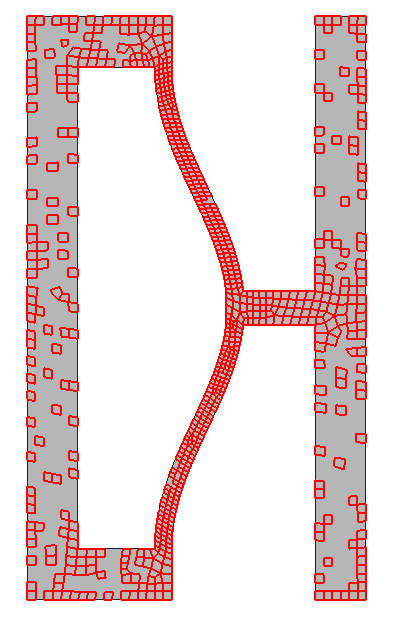
\includegraphics[width=0.35\textwidth]{FIGS/elems1.png}
    \caption{Elements containing the selected Gauss points in $\Zred$ (in red). A total of $671$ elements are retained, corresponding to $1340$ integration points.}
    \label{fig:elems1}
\end{figure}

Taken together, these observations lead to a clear conclusion. Despite the low-dimensional parametrization of the problem, the associated integrand space exhibits a high intrinsic complexity, both in terms of dimensionality and spatial distribution. As a result, the DECM  requires a large number of modes and, consequently, a large number of integration points. This directly limits the effectiveness of any fixed cubature rule.

Therefore, in the present setting, a standard hyperreduced-order model based on a fixed ECM rule is not a viable approach. The lack of strong compressibility of the integrand space prevents the construction of a sufficiently sparse integration rule, and thus precludes the possibility of achieving significant computational gains within the classical HROM framework.




\PROMPT{\input{Prompt_NumAhrom_1}}
%\input{Implementation_MATLAB_1}
\MATLAB{
The construction of the ECM integration basis is implemented in blocks. First,
the reduced displacement-gradient operator is assembled in
\href{/home/joaquin/Desktop/CURRENT_TASKS/MATLAB_CODES/FE_HROM/LARGE_STRAINS/NonLinearManifolds/OFFLINE_STAGE_nonECM_genFASTd.m}{OFFLINE\_STAGE\_nonECM\_genFASTd.m}.
For periodic boundary conditions, the relevant operator is built as
\texttt{BstRED\_l = OPERFE.Bst*OTHER\_output.DISP\_CONDITIONS.A*BasisU},
which corresponds to the product between the Gauss-point gradient operator,
the periodic lifting matrix, and the displacement basis.
}

\MATLAB{
Although the main text presents the homogenized PK1 stress through volume
averaging, the current implementation evaluates the corresponding output through
boundary reactions. The reaction-output modes are computed in
\href{/home/joaquin/Desktop/CURRENT_TASKS/MATLAB_CODES/FE_HROM/LARGE_STRAINS/NonLinearManifolds/DetermineModeReactionsOUTPUT_glo.m}{DetermineModeReactionsOUTPUT\_glo.m},
which calls
\href{/home/joaquin/Desktop/CURRENT_TASKS/MATLAB_CODES/FE_HROM/LARGE_STRAINS/NonLinearManifolds/DetermineModeHomogViaREACT.m}{DetermineModeHomogViaREACT.m}.
The resulting reaction operator is denoted in the code by \texttt{BstRED\_r}.
When reaction outputs are included in the ECM construction, this block may be
normalized by its Frobenius norm and rescaled with the Frobenius norm of the
equilibrium block, in order to balance both contributions in the SVD.
}

\MATLAB{
The flags controlling the construction are
\texttt{DATAoffline.ECMforEquilibrium} and
\texttt{DATAoffline.ECMforReactionForces}. If only equilibrium is considered,
the integrand matrix is assembled from the equilibrium block. If reaction forces
are also considered, the reaction-output block is appended to the equilibrium
block before constructing the ECM basis. If equilibrium is disabled and reaction
forces are enabled, the ECM basis is constructed only from the reaction-output
block.
}

\MATLAB{
The matrix of reduced internal-force densities is assembled in
\href{/home/joaquin/Desktop/CURRENT_TASKS/MATLAB_CODES/FE_HROM/LARGE_STRAINS/NonLinearManifolds/OFFLINE_STAGE_nonECM_genFASTd.m}{OFFLINE\_STAGE\_nonECM\_genFASTd.m}
through calls to
\href{/home/joaquin/Desktop/CURRENT_TASKS/MATLAB_CODES/FE_HROM/LARGE_STRAINS/HROM/BasisF_from_BasisStress_PK1.m}{BasisF\_from\_BasisStress\_PK1.m}.
This routine receives the reduced gradient block, or the concatenation of the
equilibrium and reaction-output blocks, together with the PK1 stress snapshots,
and returns the matrix used as input for the SVD that defines the ECM basis.
}

\MATLAB{
The basis matrix $\Ucub$ is computed in
\href{/home/joaquin/Desktop/CURRENT_TASKS/MATLAB_CODES/FE_HROM/LARGE_STRAINS/NonLinearManifolds/QbasisMatrixIntegrand_givenSNAPr.m}{QbasisMatrixIntegrand\_givenSNAPr.m}.
The SVD can be performed in the norm induced by the FE quadrature weights.
When the full matrix does not fit in memory, the partitioned implementation
\href{/home/joaquin/Desktop/CURRENT_TASKS/MATLAB_CODES/FE_HROM/LARGE_STRAINS/NonLinearManifolds/Qmatrix_LOC_forECM_cell.m}{Qmatrix\_LOC\_forECM\_cell.m}
is used. This version processes the integrand matrix by blocks and employs the
SRSVD strategy introduced in \cite{hernandez2024cecm}.
}

\MATLAB{
The same routines also implement the enrichment required to integrate the
constant function. The component of the volume vector not represented by the
current SVD basis is computed, orthonormalized if necessary, and appended to
$\Ucub$. This is the implementation counterpart of the additional volume
constraint discussed in the main text.
}

\MATLAB{
Once $\Ucub$ has been constructed, the discrete ECM problem is launched from
\href{/home/joaquin/Desktop/DiscreteECM_givenAmat.m}{DiscreteECM\_givenAmat.m}.
The actual greedy cubature algorithm is implemented in
\href{/home/joaquin/Desktop/CURRENT_TASKS/MATLAB_CODES/FE_HROM/SVDlibrary/ECM/DiscreteEmpiricalCubatureMethod.m}{DiscreteEmpiricalCubatureMethod.m},
which returns the selected Gauss points and their positive cubature weights.
}



\PROMPT{\input{Prompt_NH2}}


%\input{NH_2}
\subsection{A posteriori accuracy of the standard HROM}
\label{subsec:standard_HROM_accuracy}

We now assess the accuracy of the standard HROM obtained from the linear basis
$\PhiROM$. The comparison is performed on the training trajectories, using the FE
solution as reference. We report the relative Frobenius displacement error
$\errdisp$, together with two indicators for the homogenized PK1 stresses:
the relative Frobenius error $\errPK$ and the relative maximum error
$\errPKmax$. The values in Table~\ref{tab:standard_HROM_accuracy} correspond to
averages over the two loading trajectories in the macroscopic parameter space.

\begin{table}[H]
\centering
\caption{A posteriori errors for the standard HROM. The displacement tolerance
controls the number of retained displacement modes, while the internal-force
SVD tolerance is kept fixed at $10^{-4}$ in the ECM cases.}
\label{tab:standard_HROM_accuracy}
\begin{tabular}{cccccc}
\toprule
Case & $\varepsilon_d^{\mathrm{SVD}}$ & $\rROM$ & $\nECM$ &
$\errdisp$ & $\errPK$ \\
\midrule
Full Gauss rule & $10^{-6}$ & 52 & 5260 & $2.52\times 10^{-6}$ & $5.05\times 10^{-5}$ \\
ECM             & $10^{-6}$ & 52 & 1340 & $1.85\times 10^{-5}$ & $7.13\times 10^{-5}$ \\
ECM             & $10^{-5}$ & 37 & 1173 & $4.22\times 10^{-5}$ & $5.93\times 10^{-4}$ \\
ECM             & $10^{-4}$ & 25 & 1011 & $4.99\times 10^{-4}$ & $9.28\times 10^{-3}$ \\
\bottomrule
\end{tabular}
\end{table}

The first two rows isolate the effect of hyperreduction. With $\rROM=52$, the
use of ECM increases the displacement error from $2.52\times10^{-6}$ to
$1.85\times10^{-5}$, and the homogenized-stress error from $5.05\times10^{-5}$
to $7.13\times10^{-5}$. Thus, for this tolerance level, the ECM contribution to
the error is visible but remains small.

The more significant trend appears when the displacement basis is truncated more
aggressively. Reducing the SVD tolerance from $10^{-6}$ to $10^{-5}$ decreases
the number of modes from 52 to 37, but the number of ECM points only decreases
from 1340 to 1173. With a tolerance of $10^{-4}$, the number of modes is further
reduced to 25, while the ECM rule still requires 1011 points. This weak decrease
of $\nECM$ with $\rROM$ is consistent with the observation that the dimension of
the space spanned by the reduced internal-force densities may scale much faster
than the displacement basis itself, as discussed in \cite{bravo2024subspace}.

More importantly, the homogenized stresses are much more sensitive than the
global displacement error. With 25 modes, the average displacement error remains
below $5\times10^{-4}$, but the average PK1 stress error rises to approximately
$9.3\times10^{-3}$, with componentwise maximum errors exceeding $3\%$ in some
parts of the trajectory. This shows that the Frobenius norm of the displacement
snapshots is not, by itself, a reliable indicator of output accuracy: local
kinematic errors that are small in a global norm may have a significant impact
on stress quantities.

This effect is illustrated in Figures~\ref{fig:PK1_case25} and
\ref{fig:PK1_case37}. The response combines a relatively smooth tensile branch
with a compression branch dominated by curvature changes and buckling-like
deformation of the curved ligaments. These localized features have limited
weight in a global displacement SVD, but they are essential for reproducing the
homogenized stress. Consequently, modes that may appear secondary from a purely
Frobenius-norm viewpoint can be mechanically relevant.

\begin{figure}[H]
    \centering
    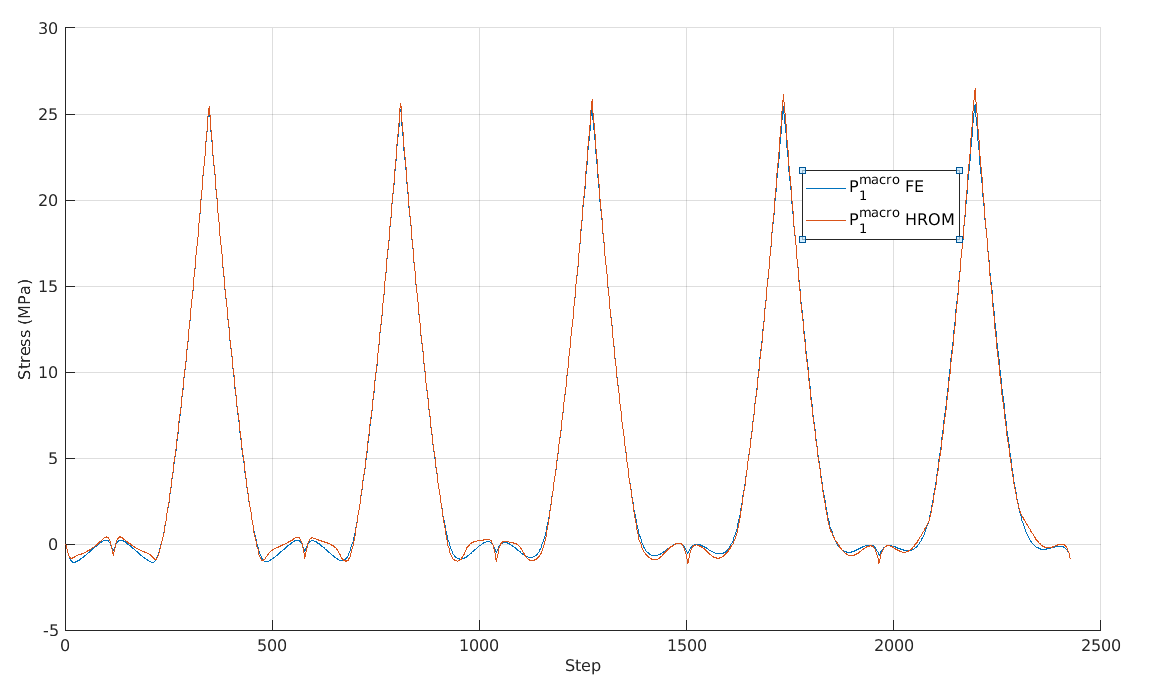
\includegraphics[width=0.78\textwidth]{FIGS/stressh1.png}
    \caption{Comparison between FE and HROM homogenized PK1 stress histories
    using 25 displacement modes. The largest discrepancies occur in the
    compression-dominated part of the trajectory, where the response is governed
    by localized changes of curvature and buckling-like deformation of the
    curved ligaments.}
    \label{fig:PK1_case25}
\end{figure}

\begin{figure}[H]
    \centering
    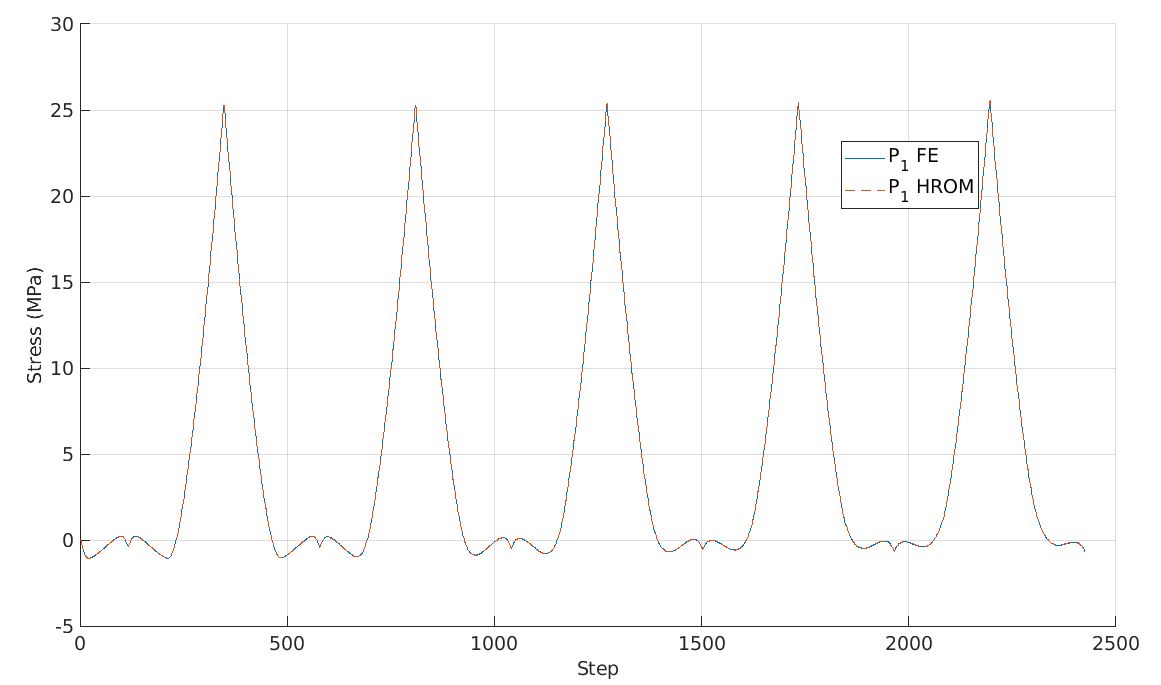
\includegraphics[width=0.78\textwidth]{FIGS/case37.png}
    \caption{Comparison between FE and HROM homogenized PK1 stress histories
    using 37 displacement modes. Increasing the number of modes substantially
    improves the stress prediction, confirming that stress accuracy requires
    retaining displacement modes associated with localized mechanisms.}
    \label{fig:PK1_case37}
\end{figure}

\MATLAB{The consistency check is performed in
\href{/home/joaquin/Desktop/CURRENT_TASKS/MATLAB_CODES/FE_HROM/LARGE_STRAINS/NonLinearManifolds/CHECK_consistency_non_gen3Rg.m}{CHECK\_consistency\_non\_gen3Rg.m}.
The same routine is used for standard and manifold HROMs; the standard HROM is
recovered as the particular case in which the nonlinear map is the identity
(\texttt{tauFUN\_identity}). Homogenized PK1 stress errors are computed in
\href{/home/joaquin/Desktop/CURRENT_TASKS/MATLAB_CODES/FE_HROM/LARGE_STRAINS/NonLinearManifolds/CompareHomogenizedPK1Stresses.m}{CompareHomogenizedPK1Stresses.m}.
The cases reported in Table~\ref{tab:standard_HROM_accuracy} correspond to
\texttt{NameInputFile = 'Data\_M3std'}, \texttt{'Data\_M3stdNH'},
\texttt{'Data\_M3std2'}, and \texttt{'Data\_M3std3'}.}


\MATLAB{
The figures shown in Section~\ref{subsec:standard_HROM_accuracy} are generated
from the MATLAB files
\href{/home/joaquin/Desktop/CURRENT_TASKS/MATLAB_CODES/TESTING_PROBLEMS_FEHROM/115_PAPER_MAW_ECM/01_METATcellHOM_2var/PK1_ECM_case4.fig}{PK1\_ECM\_case4.fig}
and
\href{/home/joaquin/Desktop/CURRENT_TASKS/MATLAB_CODES/TESTING_PROBLEMS_FEHROM/115_PAPER_MAW_ECM/01_METATcellHOM_2var/PK1_1comp_37.fig}{PK1\_1comp\_37.fig}.
}

\section{Nonlinear-manifold reduced-order model}
\label{sec:manifold_ROM}


\PROMPT{\input{ChangingCHAT_02}}


\PROMPT{\input{Prompt_MHROMov}}

%\input{MHROMov}



The numerical evidence reported in Section~\ref{subsec:standard_HROM_accuracy}
shows that the linear approximation introduced in
Eq.~\refeq{eq:standard_ROM_expansion} does not provide a sufficiently compact
description of the present problem. Although the macroscopic input space is
two-dimensional, the microscopic response involves localized changes of
curvature and buckling-like deformation of the curved ligaments, especially
along the compression branch. These features are poorly represented by a global
linear subspace: modes that carry little energy in the Frobenius norm may still
be essential for the accurate prediction of homogenized stresses.

This behavior is consistent with the Kolmogorov-width limitation of linear
projection-based reduced-order models. A solution set may be parameterized by a
small number of variables and nevertheless require a relatively large linear
space for accurate approximation. In the present case, this limitation is even
more visible at the hyperreduction level. The number of ECM points decreases
only weakly with the number of retained displacement modes, indicating that the
space of reduced internal-force and stress-output integrands has a complexity
that is not controlled directly by the dimension of the displacement subspace.
For nonlinear problems, this integrand space may grow rapidly with the number
of reduced coordinates, since the residual depends nonlinearly on the reduced
state and its projection introduces products between tangent directions and
state-dependent stress fields.

These observations motivate the replacement of the global linear subspace by a
nonlinear approximation manifold. The objective is not to abandon the structure
of the finite element equilibrium problem, but to modify the kinematic
approximation used to represent the independent displacement vector. Following
the terminology commonly used in nonlinear projection-based model reduction, we
introduce a decoder
\[
\Decod:\mathbb{R}^{\rD}\rightarrow \mathbb{R}^{\nL},
\]
and approximate the independent displacement vector as
\begin{equation}
\label{eq:dredNON}
\dred \approx \Decod(\qM),
\end{equation}
where $\qM\in\mathbb{R}^{\rD}$ denotes the nonlinear-manifold coordinates\footnote{The
meaning of the subscript $M$ will become apparent later. At this stage, it only
identifies the coordinates used to parameterize the nonlinear reduced
manifold}. The dimension $\rD$ is expected to be much smaller than the dimension $\rROM$
required by the linear ROM for comparable accuracy. Notice that the linear approximation
in Eq.~\refeq{eq:standard_ROM_expansion} is recovered as the particular case $\Decod(\qM)=\PhiROM \qM$,
up to the notational identification of $\qM$ with the standard reduced
coordinate vector $\qrom$. Thus, the nonlinear-manifold approximation is not a
different mechanical model, but a generalization of the trial space used in the
projection.

For offline construction and post-processing it is also convenient to introduce
the inverse operation, or encoder,
\[
\Encod:\mathbb{R}^{\nL}\rightarrow \mathbb{R}^{\rD},
\qquad
\qM \approx \Encod(\dred).
\]
This map assigns manifold coordinates to a given displacement snapshot. In the
present work, the encoder is used only as an offline device to parameterize the
available finite element snapshots and to organize the quantities required for
hyperreduction. The formulation below does not assume that the nonlinear
manifold is obtained from an autoencoder; the terms encoder and decoder are
used only to emphasize the analogy with latent-variable representations.

\subsection{Tangent-space projection}
\label{subsec:tangent_projection}

The nonlinear approximation in Eq.~\refeq{eq:dredNON} induces a state-dependent
space of admissible virtual displacements. Taking the first variation gives
\begin{equation}
\label{eq:virtual_dred_manifold}
\delta\dred
=
\derpar{\Decod}{\qM}(\qM)\,\delta\qM .
\end{equation}
We denote the Jacobian of the decoder by
\begin{equation}
\label{eq:PhiD_definition}
\PhiD(\qM)
:=
\derpar{\Decod}{\qM}(\qM)
\in \mathbb{R}^{\nL\times\rD}.
\end{equation}
The columns of $\PhiD(\qM)$ span the tangent space to the nonlinear
approximation manifold at the state $\Decod(\qM)$. This is the main difference
with the standard ROM: in Eq.~\refeq{eq:standard_ROM_expansion}, the test space
is the fixed linear space spanned by $\PhiROM$, whereas in the present
formulation the admissible virtual displacements depend on the current
manifold coordinate $\qM$.

The constrained finite element equilibrium equation remains that given in
Eq.~\refeq{eq:013aaa}, with the only modification being the choice of test
space. Projection onto the tangent space of the nonlinear manifold yields
\begin{equation}
\label{eq:manifold_ROM_equilibrium_FE_weights}
\sum_{g=1}^{\ngp}
\rDec{g}(\qM;\muvec)\,\wFEg{g}
=
\bm{0},
\end{equation}
where
\begin{equation}
\label{eq:rDec_definition}
\rDec{g}(\qM;\muvec)
:=
\PhiD(\qM)^T
\rFE{g}(\qM;\muvec)\!
\in \mathbb{R}^{\rD}.
\end{equation}
This formulation defines a system of $\rD$ nonlinear equations for the
manifold coordinates $\qM$. At this stage, the integration rule remains
unchanged: all $\ngp$ Gauss points are retained together with the original
finite element weights $\wFEg{g}$.


% \subsection{Hyperreduction (fixed weights)}
% \label{sec:hfixedweights}
\PROMPT{\input{Prompt_FixedWeights}}


%\input{FixedWeights}

\subsection{Fixed-weight hyperreduction on the nonlinear manifold}
\label{subsec:fixed_weight_manifold_hrom}

The expression~\eqref{eq:rDec_definition} highlights the key structural
difference with the linear setting. The scalar integrands are now obtained by
projection onto the state-dependent tangent basis $\PhiD(\qM)$, rather than
onto a fixed subspace. Nevertheless, before introducing adaptive weights, it is
useful to formulate the direct nonlinear-manifold counterpart of the standard
ECM-based HROM.

In this subsection we retain the same hyperreduction paradigm adopted in
Section~\ref{subsec:standard_HROM_accuracy}: the cubature weights are fixed,
i.e., independent of the current reduced state. Thus, the full Gauss-point
equilibrium equation~\eqref{eq:manifold_ROM_equilibrium_FE_weights} is replaced
by
\begin{equation}
\label{eq:manifold_fixed_ECM_equilibrium}
    \sum_{g\in\ZD}
    \rDec{g}(\qM;\muvec)\,\wDg{g}
    =
    \bm{0},
\end{equation}
where $\ZD\subset\{1,\ldots,\ngp\}$ is the selected set of Gauss points and
$\wDg{g}>0$ are the associated cubature weights. The superscript
$\mathcal{D}$ emphasizes that the weights are attached to the decoder-based
manifold formulation.

As in the standard HROM, we consider here the case in which the same cubature
rule is used for both the governing equilibrium equations and the output of
interest. Therefore, the homogenized PK1 stress is approximated as
\begin{equation}
\label{eq:PKmacro_manifold_fixed_rule}
    \PKmacro
    \approx
    \frac{1}{|\Omega_0|}
    \sum_{g\in\ZD}
    \PKone_g(\qM;\muvec)\,\wDg{g}.
\end{equation}
The notation $\PKone_g(\qM;\muvec)$ means that the microscopic stress is
evaluated from the decoder-reconstructed displacement
$\Alift\Decod(\qM)+\Umacro\muvec$.

The training matrix associated with the equilibrium integrands is modified
accordingly. For a single training state $({\qM}_j,\muvec_j)$, define
\begin{equation}
\label{eq:aforceD_single_state}
\aforceD({\qM}_j;\muvec_j)
=
\begin{bmatrix}
\rDec{1}({\qM}_j;\muvec_j)^T\\
\rDec{2}({\qM}_j;\muvec_j)^T\\
\vdots\\
\rDec{\ngp}({\qM}_j;\muvec_j)^T
\end{bmatrix}
\in \mathbb{R}^{\ngp\times\rD}.
\end{equation}
Collecting all training states gives
\begin{equation}
\label{eq:AforceD_training_matrix}
    \AforceD
    =
    \begin{bmatrix}
        \aforceD({\qM}_1;\muvec_1) &
        \aforceD({\qM}_2;\muvec_2) &
        \cdots &
        \aforceD({\qM}_{\nsnap};\muvec_{\nsnap})
    \end{bmatrix}
    \in \mathbb{R}^{\ngp\times(\rD\nsnap)}.
\end{equation}
This matrix is the nonlinear-manifold counterpart of
Eq.~\refeq{eq:aforce_orig}. The difference is purely structural but important:
in the standard HROM, each state contributes $\rROM$ scalar integrand fields,
one for each column of the fixed basis $\PhiROM$; in the manifold formulation,
each state contributes only $\rD$ fields, associated with the tangent basis
$\PhiD({\qM}_j)$. In favorable cases, $\rD$ can be chosen as small as the
dimension $\nmu$ of the macroscopic input space.

The stress-output matrix $\AP$ keeps the same structure as in
Eq.~\refeq{eq:Aforce_training_matrix}. What changes is the state at which the
Gauss-point stresses are evaluated: they are now computed from the
decoder-reconstructed displacement on the nonlinear manifold. If the same
cubature rule is required to approximate both equilibrium and output
quantities, the matrix used to construct the ECM basis is obtained from the
concatenation
\begin{equation}
\label{eq:manifold_fixed_ECM_training_matrix}
    \begin{bmatrix}
    \AforceD & \AP
    \end{bmatrix},
\end{equation}
with the same caveat as before regarding the relative scaling of equilibrium
and stress-output blocks.

% \begin{equation}
% \label{eq:ECM_problem}
% \begin{aligned}
%     \min_{\wPhi} \quad & \|\wPhi\|_0 \\
%     \text{s.t.} \quad & \Ucub^T \wPhi = \bFE, \\
%                       & \wPhi \ge 0,
% \end{aligned}
% \end{equation}

Once the corresponding left singular basis has been computed, the cubature
problem is formally identical to the standard ECM problem~\ref{eq:ECM_problem}. With a slight abuse
of notation, we again denote this basis by $\Ucub$ and its exact integral vector
by $\bcub= \Ucub^T\wFE$, now omitting the superscript ``FE'' for compactness. The fixed
manifold-HROM cubature rule is obtained from
\begin{equation}
\label{eq:ECM_problem_manifold_fixed}
\begin{aligned}
    \min_{\wD} \quad & \|\wD\|_0 \\
    \text{s.t.} \quad & \Ucub^T \wD = \bcub, \\
                      & \wD \ge 0 .
\end{aligned}
\end{equation}
The support of $\wD$ defines $\ZD$. Thus, after the integrand matrix has been
assembled, the construction of a fixed-weight manifold HROM follows the same
ECM machinery as in the linear case.

\subsubsection{Construction of the manifold ECM snapshots}
\label{subsubsec:manifold_ECM_snapshots}

A subtle point concerns the construction of the snapshot matrices entering
Eq.~\refeq{eq:manifold_fixed_ECM_training_matrix}. In the standard HROM this
step is essentially implicit: the FE snapshots are projected onto the fixed
linear basis and the required Gauss-point quantities are evaluated at the
corresponding reduced states. In the nonlinear-manifold setting, the same
operation requires specifying how the training states are placed on the
manifold.

One possibility is to solve the nonlinear-manifold ROM using the full Gauss
rule and then use the resulting states to assemble $\AforceD$ and $\AP$. This
is conceptually direct, but it requires an additional full-integration reduced
solve for each training configuration.

The alternative adopted here is to use the available FE snapshots. Given a
finite element displacement snapshot $\dred(\muvec_j)$, the encoder provides
the associated manifold coordinate,
\[
    {\qM}_j = \Encod(\dred(\muvec_j)).
\]
The state used for stress and internal-force evaluation is then not the raw FE
snapshot itself, but its decoder reconstruction,
\begin{equation}
\label{eq:dredD_definition}
    {\dredD}_j
    :=
    \Decod\!\left(\Encod(\dred(\muvec_j))\right).
\end{equation}
The Gauss-point strains, stresses, internal-force contributions, and tangent
projections entering $\AforceD$ and $\AP$ are evaluated from
$\Alift{\dredD}_j+\Umacro\muvec_j$. This distinction is important: the ECM
training matrix must be consistent with the approximation manifold on which
the online HROM will operate, rather than with displacement fields that do not
belong exactly to that manifold.

\begin{remark}[Input-driven manifolds in static homogenization]
\label{rem:input_driven_manifold}
There is a special situation, relevant for the present homogenization example,
in which the construction simplifies further. The macroscopic input is a
displacement-like quantity imposed through the boundary conditions, the problem
is static, and the material response is hyperelastic, so there is no dependence
on loading history or inertial effects. Under these assumptions, the
microscopic equilibrium solution is uniquely parameterized by the prescribed
macroscopic deformation. Consequently, one may choose the manifold coordinates
to coincide with the macroscopic input variables,
\[
    \qM \equiv \muvec,
    \qquad
    \rD=\nmu .
\]
This is a very specific setting and should not be interpreted as a general
property of nonlinear manifold ROMs. Its consequence, however, is important:
if the goal is only to approximate the output map
$\muvec\mapsto\PKmacro(\muvec)$, then solving the reduced equilibrium equation
is no longer necessary. In that case, the cubature rule does not need to
reproduce the manifold-projected equilibrium integrands in $\AforceD$; it only
needs to integrate accurately the stress-output fields. The matrix used to
construct $\Ucub$ is then simply $\AP$. Since $\AP$ has only
$\nstress\nsnap$ columns, instead of $(\rD+\nstress)\nsnap$ columns when both
equilibrium and output constraints are retained, the rank of the ECM basis may
be significantly smaller, and the resulting cubature rule may require fewer
integration points.
\end{remark}



\PROMPT{\input{Prompt_FWh}}

%\input{FWh_v1}
\PROMPT{\input{FWh_v2}}
%\input{FWh_v3}

\subsection{Identification of the nonlinear  manifold}
\label{subsec:manifold_identification_cell}

We now particularize the fixed-weight nonlinear-manifold HROM introduced above
to the metamaterial cell. The first step is the identification of the
nonlinear approximation manifold, namely the construction of the latent
coordinates $\qM$ and of the decoder $\Decod$. This point was deliberately
left open in the abstract formulation, since the hyperreduction strategy does
not depend on a unique choice of manifold-learning procedure.

The starting point is the same linear basis $\PhiROM\in\mathbb{R}^{\nL\times\rROM}$ used in the standard
HROM. Rather than using this basis as
the final trial space, we use it as an intermediate coordinate system in which
a nonlinear approximation manifold is constructed. The manifold approximation
is written as
\begin{equation}
\label{eq:decoder_master_slave}
    \dred
    \approx
    \Decod(\qM)
    :=
    \PhiM \Am \qM
    +
    \PhiS \Nslave(\qM).
\end{equation}
where
\begin{equation}
\label{eq:isorth}
 \PhiM^T\PhiS=\bm{0}
\end{equation}
Here $\PhiM\in\mathbb{R}^{\nL\times\rD}$ denotes the master basis,
$\PhiS\in\mathbb{R}^{\nL\times(\rROM-\rD)}$ is the complementary slave basis,
and
\[
    \Nslave:\mathbb{R}^{\rD}
    \rightarrow
    \mathbb{R}^{\rROM-\rD}
\]
is the nonlinear map that reconstructs the slave amplitudes from the master
coordinates.
%
%
% The decomposition is imposed at the level of subspaces,
%
%
%
% not by
% partitioning the original POD coefficients:
% \begin{equation}
% \label{eq:master_slave_space_decomposition}
%     \Col(\PhiROM)
%     =
%     \Col(\PhiM)\oplus \Col(\PhiS),
%     \qquad
%     \PhiM^T\PhiM=\ident,
%     \qquad
%     \PhiS^T\PhiS=\ident,
%     \qquad
%     \PhiM^T\PhiS=\bm{0}.
% \end{equation}
% The matrix $\Am$ accounts for the scaling induced by the orthonormalization of
% the master subspace.

We next describe how $\PhiM$, $\Am$, and $\qM$ are determined. Let
$\Dsnap\in\mathbb{R}^{\nL\times\nsnap}$ be the displacement snapshot matrix
introduced in Eq.~\refeq{eq:Dmatrix}. The corresponding matrix of POD
coefficients is
\[
    \Qrom
    =
    \PhiROM^T \Dsnap
    =
    \begin{bmatrix}
    \qrom_1 & \qrom_2 & \cdots & \qrom_{\nsnap}
    \end{bmatrix}
    \in\mathbb{R}^{\rROM\times\nsnap}.
\]
We also define
\[
    \Mtrain
    =
    \begin{bmatrix}
    \muvec_1 & \muvec_2 & \cdots & \muvec_{\nsnap}
    \end{bmatrix}
    \in\mathbb{R}^{\nmu\times\nsnap},
\]
where $\Mtrain$ collects the macroscopic input coordinates associated with the
training snapshots. In the present case, $\nmu=2$ and
$\muvec=(G_x^{macro},G_{xy}^{macro})^T$. We seek a linear map
\[
    \Tm\in\mathbb{R}^{\rD\times\rROM},
    \qquad
    \rD=\nmu=2,
\]
such that the reduced coordinates are mapped onto the macroscopic input
coordinates in the least-squares sense:
\begin{equation}
\label{eq:least_squares_master_coordinates}
    \Tm
    =
    \arg\min_{\widetilde{\Tm}}
    \left\|
    \widetilde{\Tm}\Qrom-\Mtrain
    \right\|_F^2 .
\end{equation}
If the residual in Eq.~\refeq{eq:least_squares_master_coordinates} is
negligible, the master coordinates can be identified with the macroscopic
input variables,
\begin{equation}
\label{eq:inpdriven}
    \qM=\Tm\qrom\approx\muvec .
\end{equation}
This is the input-driven situation anticipated in
Remark~\ref{rem:input_driven_manifold}.




The master displacement subspace associated with $\Tm$ is first obtained in
non-orthonormal form as
\begin{equation}
\label{eq:Phic_definition}
    \Phic
    =
    \PhiROM\Tm^T
    \in\mathbb{R}^{\nL\times\rD}.
\end{equation}
Indeed, since $\qM=\Tm\qrom$ and $\qrom=\PhiROM^T\dred$, one has
\[
    \qM
    =
    \Tm\PhiROM^T\dred
    =
    \Phic^T\dred .
\]
Thus, the columns of $\Phic$ define the linear functionals that extract the
master coordinates from a displacement field.

Since $\Phic$ is not necessarily orthonormal, we compute the thin SVD
\[
    \Phic=\PhiM\SigM\VM^T,
\]
and define $\PhiM$ as the orthonormal master basis. If
${\dred}_M=\PhiM\bm{a}_M$ denotes the master component of the displacement, then
\[
    \qM
    =
    \Phic^T{\dred}_M
    =
    \VM\SigM\bm{a}_M .
\]
Therefore
\[
    \bm{a}_M
    =
    \SigM^{-1}\VM^T\qM,
\]
and the matrix appearing in the decoder is
\begin{equation}
\label{eq:Am_definition}
    \Am
    =
    \SigM^{-1}\VM^T .
\end{equation}
Consequently, the master contribution in
Eq.~\refeq{eq:decoder_master_slave} is written as
$\PhiM\Am\qM$.

The slave basis is then constructed as the orthogonal complement of $\PhiM$
inside $\Col(\PhiROM)$  (the column space of $\PhiROM$). More precisely, the component of $\PhiROM$ already
represented by $\PhiM$ is removed and the remaining subspace is
orthonormalized. This yields the decomposition stated in
Eq.~\refeq{eq:isorth}, up to the truncation tolerance
used in the SVD. The slave amplitudes associated with the training snapshots
are then computed as
\[
    {\qS}_j=\PhiS^T\dred(\muvec_j),
\]
and the nonlinear closure relation
\begin{equation}
\label{eq:closure}
     \qS\approx\Nslave(\qM)
\end{equation}


is learned from the training pairs $({\qM}_j,{\qS}_j)$. This last regression
step is discussed later in Section \ref{subsubsec:RBF_slave_closure}.
The construction is inspired by nonlinear projection-based ROMs on
approximation manifolds developed by Farhat and co-workers
\cite{barnett2022quadratic,barnett2023neural,ares2026nonlinear}, but differs
in a key aspect. In the primary--secondary strategy proposed in these works,
the primary (master) variables are typically chosen as the leading POD amplitudes, which
amounts to taking $\Tm$ as a Boolean selection matrix of the form
\[
    \Tm^{\mathrm{POD}}
    =
    \begin{bmatrix}
    \ident_{\rD} & \bm{0}
    \end{bmatrix}
    \in\mathbb{R}^{\rD\times\rROM},
\]
(here    $\ident_{\rD}\in\mathbb{R}^{\rD\times\rD}$ denotes the identity matrix of size $\rD$)  so that $\qM$ consists of the first $\rD$ coefficients of $\qrom$. While this
approach is well suited to applications in which no clear low-dimensional
parametrization is available, it does not, in general, provide a direct
mechanism to guarantee minimality of the latent dimension.

% In contrast, no a priori partition of the POD coordinates is assumed here.
% The latent variables are obtained through a linear transformation $\Tm$,
% identified so as to align the reduced coordinates with physically meaningful
% macroscopic quantities while targeting the smallest possible latent dimension.
% When the least-squares relation $\qM=\Tm\qrom\approx\muvec$ is sufficiently
% accurate, the dimension of the latent space is effectively fixed by the number
% of independent macroscopic inputs. The leading-coefficient construction is thus
% recovered as a particular case, whereas the present formulation allows the
% master subspace to be any $\rD$-dimensional subspace of $\Col(\PhiROM)$
% consistent with the parametric structure of the problem.







\PROMPT{\input{Prompt_encoderH}}

%\input{EncoderH}

\PROMPT{\input{Prompt_encoderH2}}

%\input{EncoderH2}
\PROMPT{\input{Prompt_encoderH3}}

\subsubsection{Encoder}
\label{subsubsec:encoder_manifold}

We now define the encoder associated with the nonlinear manifold. In general,
for nonlinear approximation manifolds, the reduced coordinates associated with
a displacement snapshot are obtained by solving a nonlinear least-squares
problem.
\begin{equation}
\label{eq:encoder_nonlinear_LS}
    \Encod(\dred)
    =
    \arg\min_{\widetilde{\qM}\in\mathbb{R}^{\rD}}
    \frac{1}{2}
    \left\|
    \dred-\Decod(\widetilde{\qM})
    \right\|_2^2 .
\end{equation}
This is the standard construction used in nonlinear projection-based ROMs on
approximation manifolds; see, for instance, the Gauss--Newton encoder
procedure described in \cite{ares2026nonlinear}. The stationarity condition
associated with Eq.~\refeq{eq:encoder_nonlinear_LS} reads
\begin{equation}
\label{eq:encoder_normal_equation}
    \Jdec(\qM)^T
    \left[
    \Decod(\qM)-\dred
    \right]
    =
    \bm{0},
    \qquad
    \Jdec(\qM):=
    \derpar{\Decod}{\qM}(\qM).
\end{equation}

For the decoder used here,
\[
    \Decod(\qM)
    =
    \PhiM\Am\qM+\PhiS\Nslave(\qM),
\]
the tangent matrix is
\begin{equation}
\label{eq:Jdec_master_slave}
    \Jdec(\qM)
    =
    \PhiM\Am
    +
    \PhiS
    \derpar{\Nslave}{\qM}(\qM).
\end{equation}
Substituting Eq.~\refeq{eq:Jdec_master_slave} into
Eq.~\refeq{eq:encoder_normal_equation} gives
\begin{equation}
\label{eq:encoder_normal_expanded}
\begin{aligned}
&
\left(
    \Am^T\PhiM^T
    +
    \derpar{\Nslave}{\qM}(\qM)^T\PhiS^T
\right)
\left[
    \PhiM\Am\qM
    +
    \PhiS\Nslave(\qM)
    -
    \dred
\right]
=
\bm{0}.
\end{aligned}
\end{equation}
Using the orthogonality of the master and slave bases, this expression reduces
to
\begin{equation}
\label{eq:encoder_normal_split}
    \Am^T
    \left(
        \Am\qM-\PhiM^T\dred
    \right)
    +
    \derpar{\Nslave}{\qM}(\qM)^T
    \left(
        \Nslave(\qM)-\PhiS^T\dred
    \right)
    =
    \bm{0}.
\end{equation}
Equation~\refeq{eq:encoder_normal_split} shows explicitly why the exact
encoder is nonlinear: the slave contribution enters through the derivative of
the nonlinear map. To interpret this term, let the manifold approximation be
written as
\begin{equation}
\label{eq:decoder_with_error}
    \dred
    =
    \PhiM\Am\qM
    +
    \PhiS\Nslave(\qM)
    +
    \errMan ,
\end{equation}
where $\errMan\in\mathbb{R}^{\nL}$ denotes the manifold approximation error.
Premultiplication by $\PhiS^T$ gives
\[
    \PhiS^T\dred
    =
    \Nslave(\qM)
    +
    \PhiS^T\errMan ,
\]
and therefore
\[
    \Nslave(\qM)-\PhiS^T\dred
    =
    -\PhiS^T\errMan .
\]
Hence, the second term in Eq.~\refeq{eq:encoder_normal_split} is directly
controlled by the manifold approximation error. When the manifold
representation is sufficiently accurate, this contribution becomes small and
the stationarity condition reduces approximately to
\[
    \Am^T
    \left(
        \Am\qM-\PhiM^T\dred
    \right)
    =
    \bm{0},
\]
which yields
\begin{equation}
\label{eq:encoder_explicit}
    \qM
    =
    \Am^{-1}\PhiM^T\dred .
\end{equation}
Empirically, this simplified encoder has been found sufficiently accurate for
the present application.

\MATLAB{
The encoder is called in
\href{/home/joaquin/Desktop/CURRENT_TASKS/MATLAB_CODES/FE_HROM/LARGE_STRAINS/NonLinearManifolds/OFFLINE_STAGE_nonECM_2var.m}{OFFLINE\_STAGE\_nonECM\_2var.m}
through
\href{/home/joaquin/Desktop/CURRENT_TASKS/MATLAB_CODES/FE_HROM/LARGE_STRAINS/NonLinearManifolds/Encoder1MasterMode_Gen.m}{Encoder1MasterMode\_Gen.m}.
The implementation computes the projection of the displacement snapshots onto
the master basis, rescales the result with
\texttt{DATA\_evaluateTAU\_and\_DER.Am}, and obtains the master coordinates.
The nonlinear decoder is implemented through the ROM-coordinate vector
$\tauvec(\qM)$, so that
\[
    \Decod(\qM)=\PhiROM\,\tauvec(\qM).
\]
With the present master--slave convention,
\[
    \tauvec(\qM)
    =
    \begin{bmatrix}
    \Am\qM\\
    \Nslave(\qM)
    \end{bmatrix}.
\]
The function
\href{/home/joaquin/Desktop/CURRENT_TASKS/MATLAB_CODES/FE_HROM/LARGE_STRAINS/NonLinearManifolds/EvalTauSlaveRBF_Online.m}{EvalTauSlaveRBF\_Online.m}
evaluates $\tauvec(\qM)$ and, when requested, its derivatives. Its Jacobian is
\[
    \derpar{\tauvec}{\qM}
    =
    \begin{bmatrix}
    \Am\\
    \derpar{\Nslave}{\qM}
    \end{bmatrix}
    \in\mathbb{R}^{(\rD+\nS)\times\rD},
\]
where $\nS$ denotes the number of slave amplitudes. The corresponding decoder
Jacobian is therefore
\[
    \derpar{\Decod}{\qM}
    =
    \PhiROM
    \derpar{\tauvec}{\qM}.
\]
The second derivative of $\tauvec$ is a third-order tensor:
\[
    \derpar{^2\tauvec_i}{{\qM}_j\,\partial {\qM}_k},
    \qquad
    i=1,\ldots,\rD+\nS,
    \quad
    j,k=1,\ldots,\rD.
\]
In the implementation, this tensor is stored as
\texttt{d2tau\_dqM2(i,j,k)}. Since the master block $\Am\qM$ is linear, its
second derivative is zero; only the slave block contributes, namely
\[
    \derpar{^2\tauvec}{\qM^2}
    =
    \begin{bmatrix}
    \bm{0}\\
    \derpar{^2\Nslave}{\qM^2}
    \end{bmatrix}.
\]
}


\subsection{Regression by Radial basis functions}
\label{subsubsec:RBF_slave_closure}

 \PROMPT{\input{Prompt_RBFs}}


 %\input{RBFs_1}
 \PROMPT{\input{Prompt_RBFs_2}}
 %\input{RBFs_2}
 %\input{RBFs_3}
  \PROMPT{\input{Prompt_RBFs_3}}

The remaining ingredient in the decoder is the nonlinear closure
$\qS\approx\Nslave(\qM)$. Once the master coordinates have been fixed, this
closure is constructed from the training pairs $({\qM}_j,{\qS}_j)$ obtained in
Section~\ref{subsec:manifold_identification_cell}. Several choices are possible.
Deep feed-forward neural networksare now widely used in nonlinear manifold ROMs, particularly in
problems involving high-dimensional latent spaces or strongly nonlinear
manifold geometries
\cite{barnett2023neural}.In the present problem, however, the latent space is only two-dimensional and
is approximately identified with the structured macroscopic parameter grid.
This makes simpler differentiable interpolants attractive, including
tensor-product spline constructions on Cartesian grids and radial basis
functions. We adopt the latter option.


The first stage is to subsample the snapshots\footnote{The finite element
trajectories are sampled densely in pseudo-time in order to ensure robust
Newton convergence. Consecutive snapshots are therefore often highly
correlated in master space, so using all of them as RBF centers would increase
the online cost and may deteriorate the conditioning of the kernel matrix
without providing significant additional information.}. In this problem, since the latent coordinates are approximately aligned with the Cartesian
macroscopic parameter grid, the subsampling can be carried out simply at the
grid level by selecting one point every prescribed number of rows and columns.
Let $\{{\qMc}_k\}_{k=1}^{\nM}$ denote the resulting set of retained RBF
centers, where $\nM\le\nsnap$ is the number of retained samples, and let
$\ellRBF=(\ell_1,\ell_2)^T$ be the anisotropic length-scale vector. The Gaussian kernel is written as
\begin{equation}
\label{eq:RBF_kernel}
    \psirbf(\qM,{\qMc}_k)
    =
    \exp\!\left[
    -
    \left(
    \frac{q_{M,1}-q^c_{M,1,k}}{\ell_1}
    \right)^2
    -
    \left(
    \frac{q_{M,2}-q^c_{M,2,k}}{\ell_2}
    \right)^2
    \right].
\end{equation}









For a new master point $\qM$, let
\[
    \PsiRBF(\qM)
    =
    \begin{bmatrix}
    \psirbf(\qM,{\qMc}_1) &
    \cdots &
    \psirbf(\qM,{\qMc}_{\nM})
    \end{bmatrix}^T
    \in
    \mathbb{R}^{\nM}
\]
denote the vector of Gaussian kernel evaluations with respect to the retained
RBF centers. The slave amplitudes are then approximated as
\begin{equation}
\label{eq:RBF_slave_map}
    \Nslave(\qM)
    =
    \sS
    \left(
    \alphRBF^T\PsiRBF(\qM)
    +
    \betaRBF^T\pRBF(\qM)
    \right).
\end{equation}
Here
\[
    \sS=\operatorname{diag}(s_1,\ldots,s_{\nS}),
    \qquad
    s_i=
    \left(
    \frac{1}{\nM}
    \sum_{k=1}^{\nM}
    \left(q^{(k)}_{S,i}\right)^2
    \right)^{1/2},
\]
contains characteristic RMS amplitudes of the slave coordinates, used to
normalize the multi-output regression problem and improve conditioning. The
matrix $\alphRBF\in\mathbb{R}^{\nM\times\nS}$ collects the RBF coefficients,
whereas $\betaRBF\in\mathbb{R}^{\np\times\nS}$ contains the coefficients of
the optional polynomial correction $\pRBF(\qM)\in\mathbb{R}^{\np}$  (both $\alphRBF$ and $\betaRBF$ are obtained in the offline stage, as explained in the following). In the
present implementation, this correction may be absent, constant, or affine; in
the affine case,
\[
    \pRBF(\qM)
    =
    \begin{bmatrix}
    1 & q_{M,1} & q_{M,2}
    \end{bmatrix}^T .
\]

\subsubsection{Determination of RBFs parameters in the offline stage}

Let
\[
    \Qslave
    =
    \begin{bmatrix}
    {\qS}_1 & {\qS}_2 & \cdots & {\qS}_{\nM}
    \end{bmatrix}
    \in
    \mathbb{R}^{\nS\times\nM}
\]
collect the slave amplitudes associated with the retained RBF centers. The
corresponding normalized slave-coordinate matrix is
\[
    \Qslavehat
    =
    \sS^{-1}\Qslave
    \in
    \mathbb{R}^{\nS\times\nM}.
\]
The RBF coefficients are obtained offline by solving
\begin{equation}
\label{eq:RBF_augmented_system}
\begin{bmatrix}
\Krbf+\lambda\ident & \bm{P}\\
\bm{P}^T & \bm{0}
\end{bmatrix}
\begin{bmatrix}
\alphRBF\\
\betaRBF
\end{bmatrix}
=
\begin{bmatrix}
\Qslavehat^T\\
\bm{0}
\end{bmatrix},
\end{equation}
where $\lambda$ is a Tikhonov regularization parameter. The matrix
$\Krbf\in\mathbb{R}^{\nM\times\nM}$ is the Gaussian kernel matrix evaluated
at the retained centers,
\[
    (\Krbf)_{ij}
    =
    \psirbf({\qMc}_i,{\qMc}_j),
    \qquad
    i,j=1,\ldots,\nM,
\]
and $\PRBF\in\mathbb{R}^{\nM\times\np}$ is the polynomial matrix,
\[
    \PRBF
    =
    \begin{bmatrix}
    \pRBF({\qMc}_1)^T\\
    \pRBF({\qMc}_2)^T\\
    \vdots\\
    \pRBF({\qMc}_{\nM})^T
    \end{bmatrix}.
\]
All slave outputs are fitted simultaneously using the same kernel matrix.

%
%
%
% $\Krbf\in\mathbb{R}^{\nM\times\nM}$ is the Gaussian kernel matrix evaluated
% at the retained centers, and $\bm{P}\in\mathbb{R}^{\nM\times \np}$ is the
% polynomial matrix. All slave outputs are fitted simultaneously using the same
% kernel matrix.


The differentiability of the RBF map is essential because the tangent matrix of
the decoder requires $\partial\Nslave/\partial\qM$, and Newton-type procedures
may also require second derivatives. Let
\[
    \DPsiRBF(\qM)
    :=
    \derpar{\PsiRBF}{\qM}(\qM)
    \in\mathbb{R}^{\nM\times\rD}.
\]
For the Gaussian kernel in Eq.~\refeq{eq:RBF_kernel}, its entries are
\[
    \left(\DPsiRBF(\qM)\right)_{ka}
    =
    \derpar{\psirbf(\qM,{\qMc}_k)}{q_{M,a}}
    =
    -\,2\,
    \frac{q_{M,a}-q^c_{M,a,k}}{\ell_a^2}
    \psirbf(\qM,{\qMc}_k),
    \qquad
    a=1,\ldots,\rD .
\]
Therefore, differentiating Eq.~\refeq{eq:RBF_slave_map} gives
\begin{equation}
\label{eq:RBF_slave_jacobian}
    \derpar{\Nslave}{\qM}(\qM)
    =
    \sS
    \left[
    \alphRBF^T\DPsiRBF(\qM)
    +
    \betaRBF^T
    \derpar{\pRBF}{\qM}(\qM)
    \right]
    \in\mathbb{R}^{\nS\times\rD}.
\end{equation}

The second derivative is a third-order tensor. For each center $k$, the Hessian
of the Gaussian kernel is
\[
    \derpar{^2\psirbf(\qM,{\qMc}_k)}
           {q_{M,a}\,\partial q_{M,b}}
    =
    \left[
    4\,
    \frac{
    (q_{M,a}-q^c_{M,a,k})(q_{M,b}-q^c_{M,b,k})
    }{\ell_a^2\ell_b^2}
    -
    2\,\frac{\delta_{ab}}{\ell_a^2}
    \right]
    \psirbf(\qM,{\qMc}_k),
\]
where $\delta_{ab}$ is the Kronecker delta. Hence, for each slave component
$i=1,\ldots,\nS$,
\begin{equation}
\label{eq:RBF_slave_hessian}
    \derpar{^2(\Nslave)_i}{q_{M,a}\,\partial q_{M,b}}
    =
    s_i
    \left[
    \sum_{k=1}^{\nM}
    (\alphRBF)_{ki}
    \derpar{^2\psirbf(\qM,{\qMc}_k)}
           {q_{M,a}\,\partial q_{M,b}}
    +
    \sum_{m=1}^{\np}
    (\betaRBF)_{mi}
    \derpar{^2(\pRBF)_m}{q_{M,a}\,\partial q_{M,b}}
    \right].
\end{equation}
In the affine polynomial case used here, the second derivative of
$\pRBF$ is zero. Thus the Hessian tensor is entirely determined by the
Gaussian kernels. In the implementation, the Jacobian is stored as an
$\nS\times\rD$ matrix and the second derivative as an
$\nS\times\rD\times\rD$ array, with the last two indices corresponding to
the two differentiation directions in master space.

\MATLAB{
The RBF closure $\qS=\Nslave(\qM)$ is constructed offline in
\href{/home/joaquin/Desktop/CURRENT_TASKS/MATLAB_CODES/FE_HROM/LARGE_STRAINS/NonLinearManifolds/RegressionViaRBF_master_slave.m}{RegressionViaRBF\_master\_slave.m}.
The routine uses the master and slave training matrices, optionally performs
structured subsampling of the two-dimensional master grid, computes anisotropic
Gaussian length scales, normalizes each slave amplitude by its RMS value, and
solves a regularized augmented RBF system. This is the implementation
counterpart of Eqs.~\refeq{eq:RBF_kernel}--\refeq{eq:RBF_augmented_system}.
Online evaluation is performed in
\href{/home/joaquin/Desktop/CURRENT_TASKS/MATLAB_CODES/FE_HROM/LARGE_STRAINS/NonLinearManifolds/EvalSlaveRBF_Online.m}{EvalSlaveRBF\_Online.m},
which returns $\Nslave(\qM)$, its Jacobian
$\partial\Nslave/\partial\qM$, and its second derivative tensor
$\partial^2\Nslave/\partial\qM^2$. This function is called by
\href{/home/joaquin/Desktop/CURRENT_TASKS/MATLAB_CODES/FE_HROM/LARGE_STRAINS/NonLinearManifolds/EvalTauSlaveRBF_Online.m}{EvalTauSlaveRBF\_Online.m},
where the full ROM-coordinate map $\tauvec(\qM)$ and its derivatives are
assembled.
}
\MATLAB{
The structured subsampling of the master space is implemented in
\href{/home/joaquin/Desktop/CURRENT_TASKS/MATLAB_CODES/FE_HROM/LARGE_STRAINS/NonLinearManifolds/SubsamplingMasterSpace.m}{SubsamplingMasterSpace.m}.
Rather than selecting centers randomly, the routine exploits the Cartesian
structure of the parameter grid and retains one point every prescribed number
of rows and columns. This reduces the number of RBF centers, improves the
conditioning of the Gaussian kernel matrix, and avoids excessive clustering of
highly correlated snapshots originating from densely sampled Newton trajectories.
}


\subsection{Numerical assessment}




\PROMPT{\input{Prompt_MasterSlav_1}}

%\input{MHROM_nass1}
\subsubsection{Numerical characterization of the  manifold solution}
\label{subsec:num_char_fixed_manifold}

We now characterize the nonlinear-manifold approximation constructed for the
metamaterial cell. The starting point is the same displacement snapshot matrix
used in the standard HROM, and the same reference tolerance
$\varepsilon_d^{\mathrm{SVD}}=10^{-6}$. Thus, the initial linear basis is
\[
    \PhiROM\in\mathbb{R}^{3018\times 52}.
\]
The purpose of the manifold construction is not to use these $52$ coordinates
as independent unknowns, but to identify a two-dimensional master
parameterization and to reconstruct the remaining amplitudes through the
nonlinear closure $\qS\approx\Nslave(\qM)$.

The least-squares problem~\eqref{eq:least_squares_master_coordinates} gives a
relative residual equal to $3.09\times10^{-7}$. This confirms that, for the
present dataset, the master coordinates $\qM$ induced by the master basis
$\PhiM$ can be identified with the prescribed macroscopic input vector
$\muvec$, according to Eq.~\eqref{eq:inpdriven} (i.e., $\qM \approx \muvec$). Hence, this case falls within
the input-driven setting anticipated in Remark~\ref{rem:input_driven_manifold}:
the latent dimension is fixed by the two independent macroscopic inputs,
namely $\rD=\nmu=2$.

The deformed shapes of the resulting master modes ${\PhiM}_1$ and ${\PhiM}_2$ are shown in Fig.~\ref{fig:master_modes_manifold}.
They should not be interpreted in the same way as the leading POD modes of
Fig.~\ref{fig:ROM_modes}. Although the first mode displays a deformation
pattern broadly associated with horizontal compression/stretching, and the
second one contains a shear-like signature, their main role is not modal
energy ordering. Rather, they define the physical displacement directions whose
amplitudes are placed in direct correspondence with the macroscopic input
coordinates, up to the scaling matrix (obtained in turn from   Eq. \refeq{eq:Am_definition})
\[
    \Am =
    10^{-1}
    \begin{bmatrix}
    -3.9962 &  0.21588\\
    -0.34716 & -6.4264
    \end{bmatrix}.
\]
The remaining $\rROM-\rD = 52-2 = 50$ modes span the slave space, i.e. the
orthogonal complement of the master subspace inside $\Col(\PhiROM)$. The deformed shapes of some of such slave modes are
shown in Fig.~\ref{fig:slave_modes_manifold} for illustration purposes.

\begin{figure}[H]
    \centering
    \begin{subfigure}{0.3\textwidth}
        \centering
        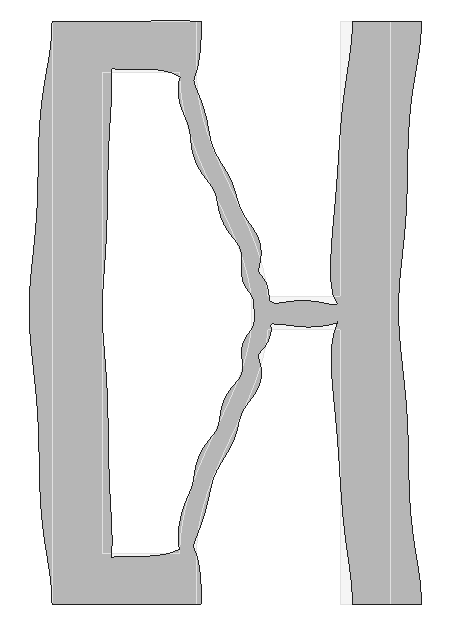
\includegraphics[width=\textwidth]{FIGS/m1m.png}
        \caption{1st master mode (${\PhiM}_1$).}
    \end{subfigure}
    \hspace{0.04\textwidth}
    \begin{subfigure}{0.3\textwidth}
        \centering
        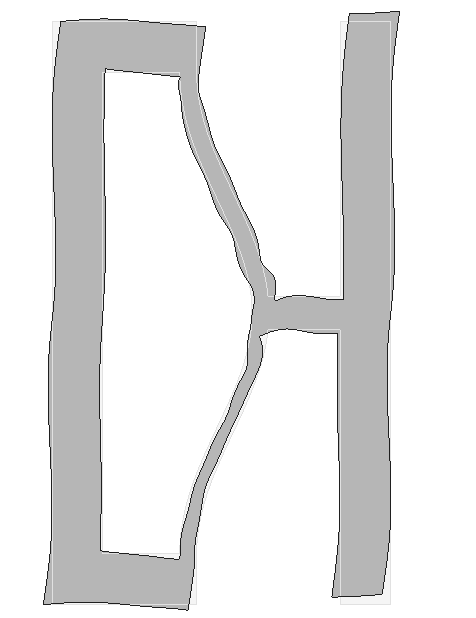
\includegraphics[width=\textwidth]{FIGS/m2m.png}
        \caption{2nd master mode (${\PhiM}_2$).}
    \end{subfigure}
    \caption{Master modes obtained from the least-squares identification of
    the two-dimensional latent space. The modes are not selected by POD energy
    ordering, but by their ability to induce amplitudes aligned with the
    macroscopic input coordinates.}
    \label{fig:master_modes_manifold}
\end{figure}

\begin{figure}[H]
    \centering
    \begin{subfigure}{0.23\textwidth}
        \centering
        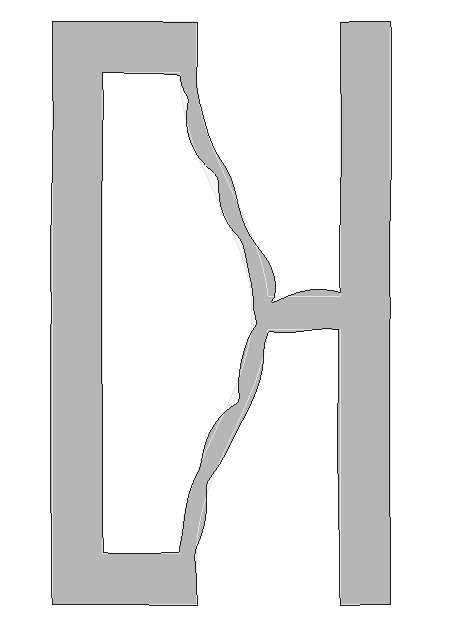
\includegraphics[width=\textwidth]{FIGS/slv1.png}
        \caption{Slave mode 1 (${\PhiS}_1$)}
    \end{subfigure}
    \begin{subfigure}{0.23\textwidth}
        \centering
        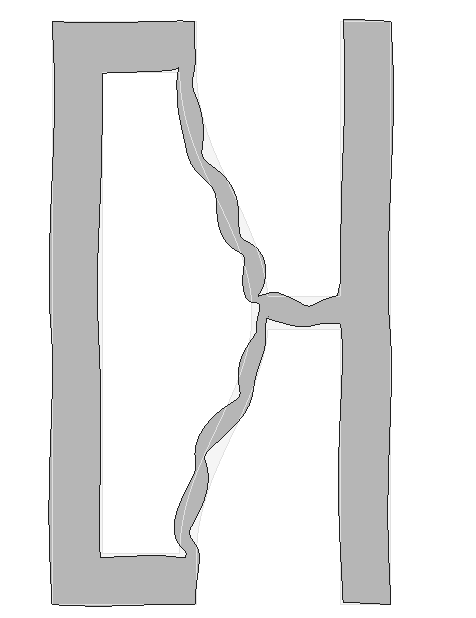
\includegraphics[width=\textwidth]{FIGS/slv5.png}
        \caption{Slave mode 6 (${\PhiS}_6$).}
    \end{subfigure}
    \begin{subfigure}{0.23\textwidth}
        \centering
        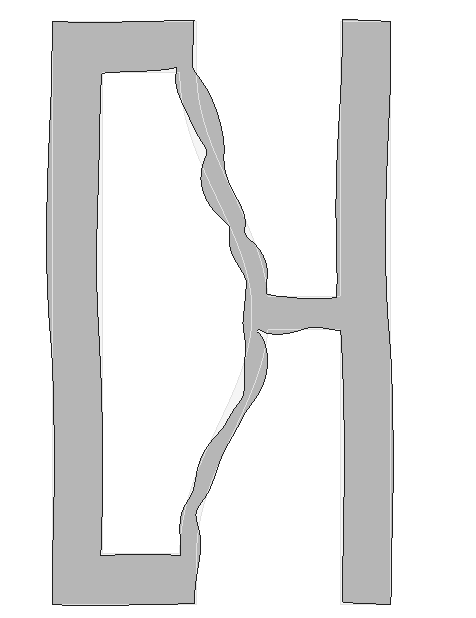
\includegraphics[width=\textwidth]{FIGS/slv13.png}
        \caption{Slave mode 13  (${\PhiS}_{13}$).}
    \end{subfigure}
    \begin{subfigure}{0.2\textwidth}
        \centering
        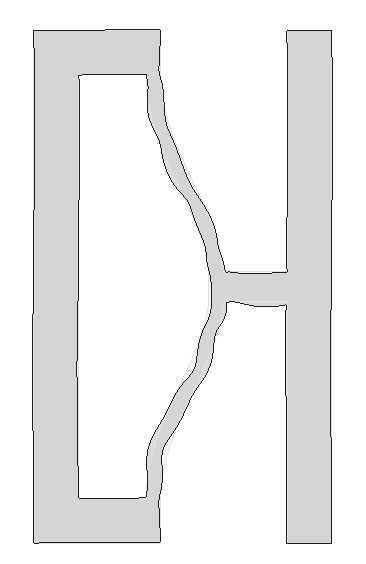
\includegraphics[width=\textwidth]{FIGS/slv44.png}
        \caption{Slave mode 44  (${\PhiS}_{44}$).}
    \end{subfigure}
    \caption{Slave modes  ${\PhiS}_1$, ${\PhiS}_6$, ${\PhiS}_{13}$ and ${\PhiS}_{44}$.  The amplitudes of these modes
    are reconstructed through the nonlinear closure
    ${\qS}_j\approx{\Nslave}_j(\qM)$.}
    \label{fig:slave_modes_manifold}
\end{figure}

The closure is built with the RBF approximation described in
Section~\ref{subsubsec:RBF_slave_closure}. The full dataset contains $4851$
training pairs, from which $\nM=1540$ centers are retained after structured
subsampling. The subsampling frequency is $[3,1]$, so that every third point is
retained along the first master direction, while all points are retained along
the second one. The length-scale factors are chosen\footnote{These values are obtained from the user-prescribed factors
$[3,3]$ by multiplying the average spacing between neighboring retained RBF
centers along each master direction. Thus, the parameters $3$ and $3$ do not
define the length scales directly, but rather the number of characteristic
point spacings used to determine the effective Gaussian support radius in each
direction.} as
\[
    \ellRBF =
    \begin{bmatrix}
    3.3013\times 10^{-2}\\
    1.5789\times 10^{-2}
    \end{bmatrix}.
\]
     Tikhonov parameter is set to $\lambda=10^{-10}$,  and the
 polynomial correction is parabolic.

With these parameters, the relative prediction error on the retained RBF
centers is $4.30\times10^{-6}$, while the reconstruction error over the full
dataset is $1.03\times10^{-4}$. This distinction is relevant: the first number
measures the interpolation quality on the subsampled centers, whereas the
second one measures the ability of the RBF closure to reconstruct all slave
amplitudes over the original dataset.

For comparison, reducing the length-scale factors by a factor $2/3$ gives a much
smaller residual on the retained centers, with prediction error
$1.37\times10^{-10}$, but increases the full-dataset reconstruction error to
$4.86\times10^{-4}$. Thus, although the shorter length scale interpolates the
retained centers more tightly, it produces a less accurate reconstruction away
from them. The first choice   is therefore retained, since it provides the
better global reconstruction over the complete training set and a smoother
closure in master space.
Figures~\ref{fig:RBF_slave_surfaces_1} and
\ref{fig:RBF_slave_surfaces_2} give a concrete visualization of the closure
relation $\qS\approx\Nslave(\qM)$. The black markers indicate the retained RBF
centers. The plotted surfaces show that
the dependence on the two master coordinates is smooth and single-valued over
the sampled domain. This supports the chosen parameterization: once the master
coordinates are identified with the macroscopic inputs, the remaining slave
amplitudes can be regarded as regular functions of $\qM$.
\begin{figure}[H]
    \centering
    \begin{subfigure}{0.48\textwidth}
        \centering
        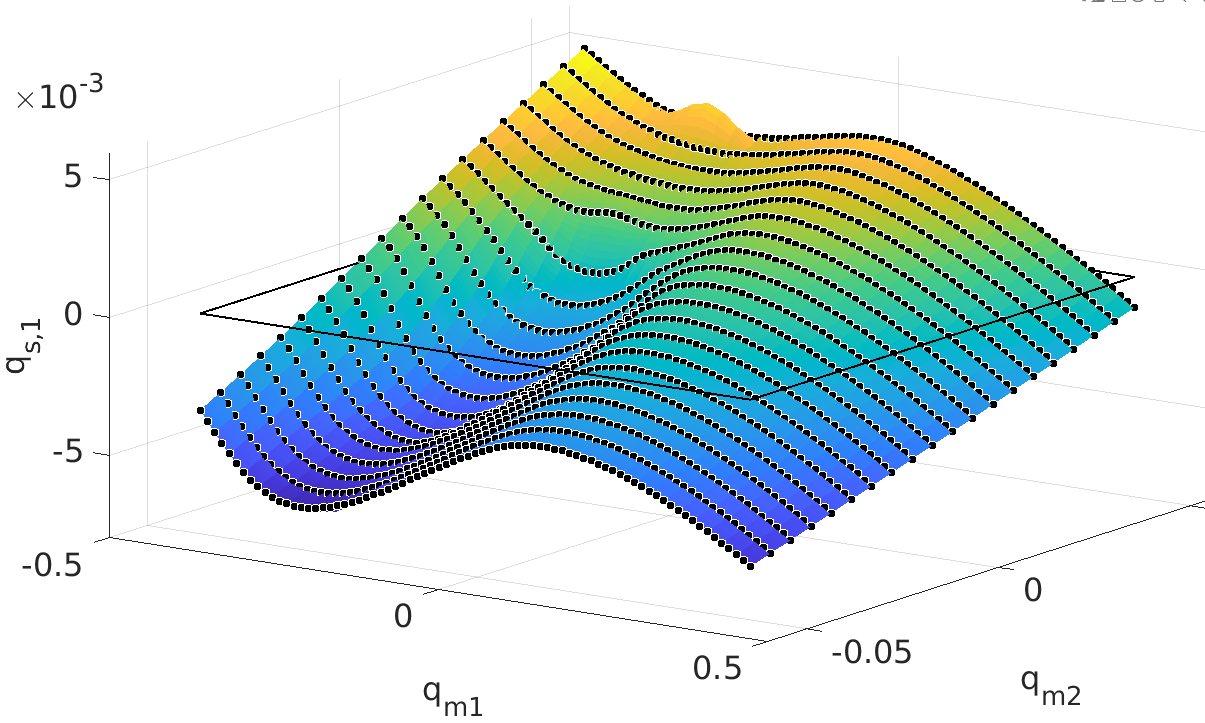
\includegraphics[width=\textwidth]{FIGS/rbf1.png}
        \caption{Slave amplitude 1.}
    \end{subfigure}
    \hspace{0.02\textwidth}
    \begin{subfigure}{0.48\textwidth}
        \centering
        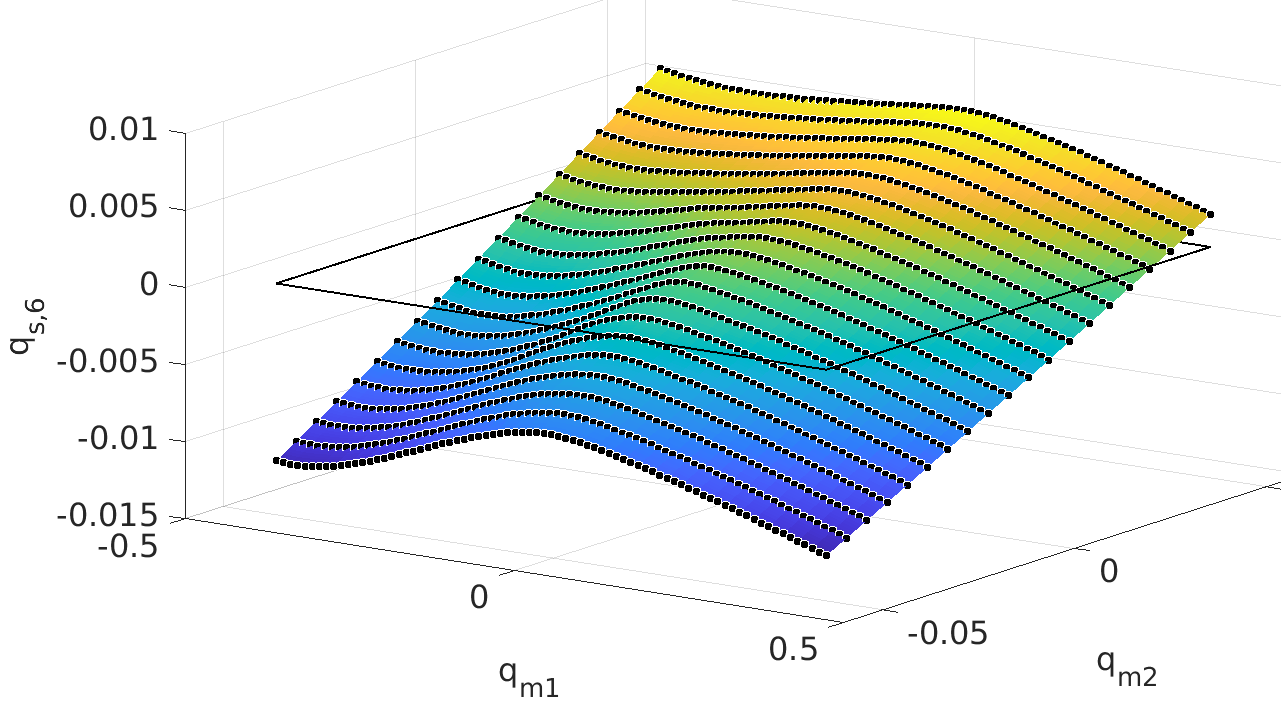
\includegraphics[width=\textwidth]{FIGS/rbf6.png}
        \caption{Slave amplitude 6.}
    \end{subfigure}
    \caption{RBF reconstruction of   slave amplitudes ${\qS}_{1}$ and ${\qS}_6{}$ over the
    two-dimensional master space. The black markers denote the retained RBF
    centers.}
    \label{fig:RBF_slave_surfaces_1}
\end{figure}

\begin{figure}[H]
    \centering
    \begin{subfigure}{0.48\textwidth}
        \centering
        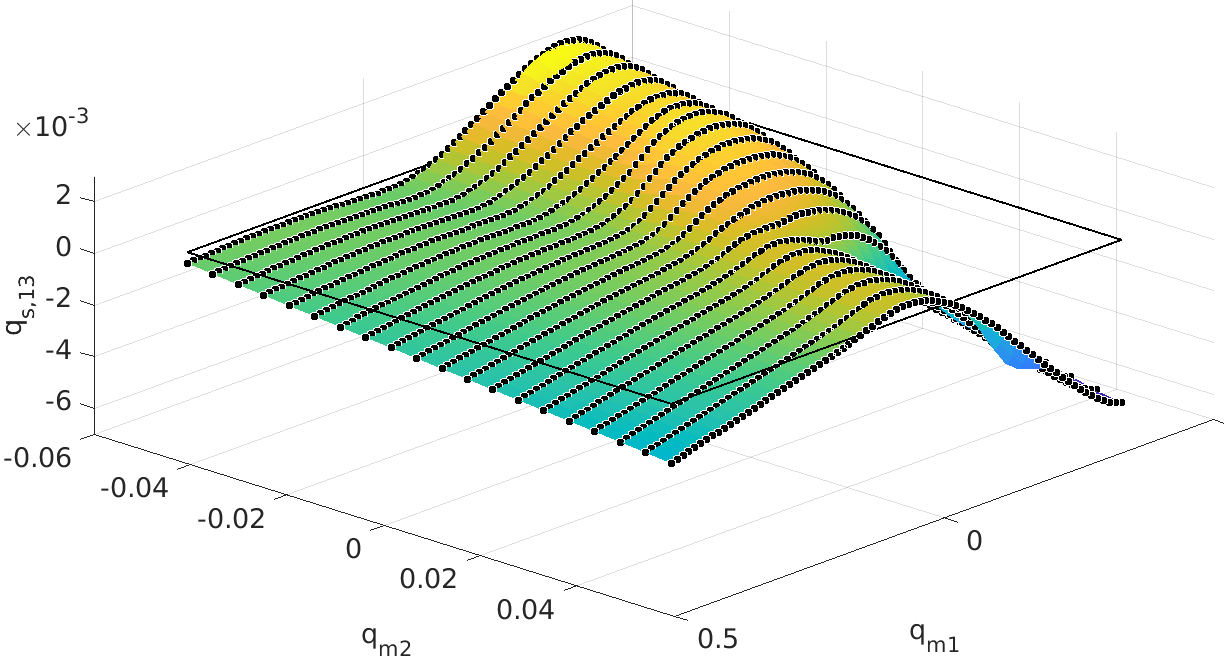
\includegraphics[width=\textwidth]{FIGS/rbf13.png}
        \caption{Slave amplitude 13.}
    \end{subfigure}
    \hspace{0.02\textwidth}
    \begin{subfigure}{0.48\textwidth}
        \centering
        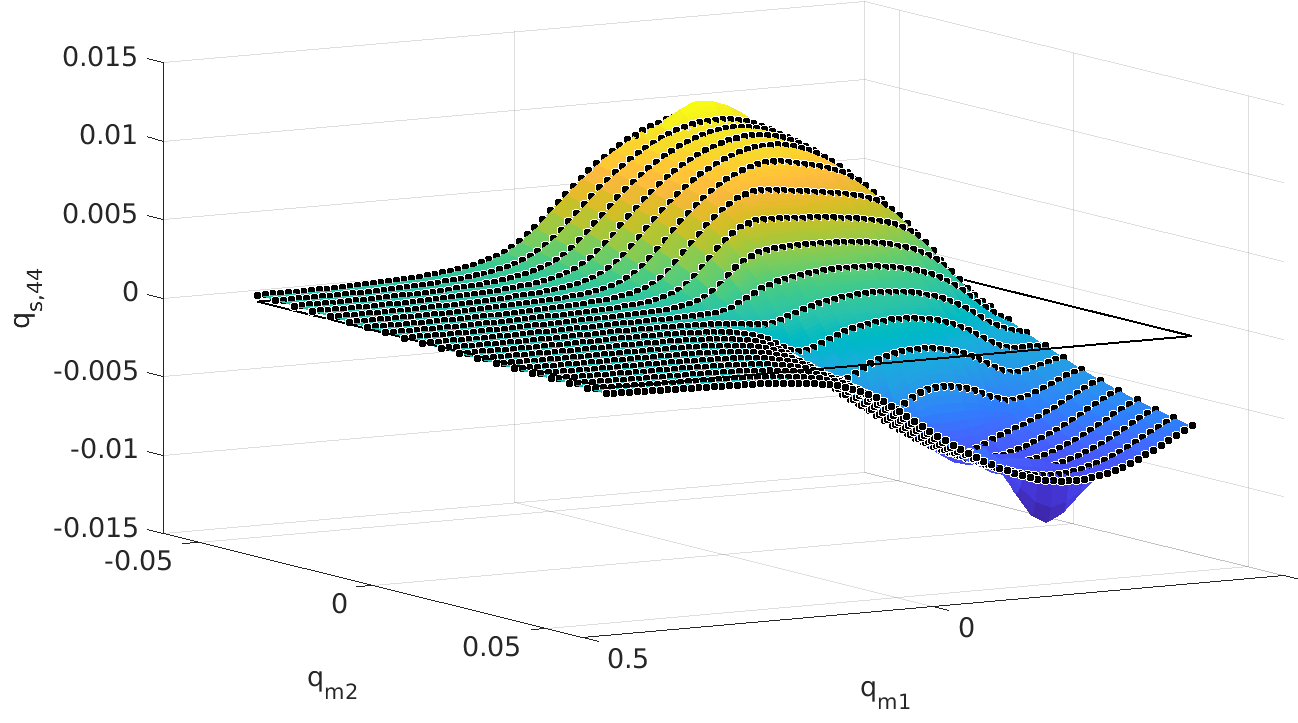
\includegraphics[width=\textwidth]{FIGS/rbf44.png}
        \caption{Slave amplitude 44.}
    \end{subfigure}
    \caption{Additional examples of RBF-reconstructed slave amplitudes. }
    \label{fig:RBF_slave_surfaces_2}
\end{figure}


\MATLAB{
The fixed-weight manifold HROM for the metamaterial cell is launched from
\href{/home/joaquin/Desktop/CURRENT_TASKS/MATLAB_CODES/TESTING_PROBLEMS_FEHROM/115_PAPER_MAW_ECM/01_METATcellHOM_2var/Run_HOMOG_2p.m}{Run\_HOMOG\_2p.m}.
The input file is
\href{/home/joaquin/Desktop/CURRENT_TASKS/MATLAB_CODES/TESTING_PROBLEMS_FEHROM/115_PAPER_MAW_ECM/01_METATcellHOM_2var/DATAINPUTS/Data_M3_hyperSTD.m}{Data\_M3\_hyperSTD.m}.
The manifold option is activated with
\texttt{DATA\_interp.METHOD\_SELECT\_REFERENCE\_MODE = 'TWO\_VARIABLES'}.
The fixed-weight hyperreduction setting is selected with
\texttt{DATAoffline.Hyperreduction\_METHOD\_projection = 'STANDARD'}.
The identification $\qM\equiv\muvec$ is imposed through
\texttt{DATA\_interp.MethodSelectMasterModes\_2var = 'LeastSquaresParametricDomain'}.
Since only the output cubature is used in this case, the flags are set as
\texttt{DATAoffline.ECMforReactionForces = true} and
\texttt{DATAoffline.ECMforEquilibrium = false}.
The offline operations are carried out in
\href{/home/joaquin/Desktop/CURRENT_TASKS/MATLAB_CODES/FE_HROM/LARGE_STRAINS/NonLinearManifolds/OFFLINE_STAGE_nonECM_2var.m}{OFFLINE\_STAGE\_nonECM\_2var.m}.
The least-squares construction of $\Tm$, $\Phic$, $\PhiM$, and $\Am$ is
implemented in
\href{/home/joaquin/Desktop/CURRENT_TASKS/MATLAB_CODES/FE_HROM/LARGE_STRAINS/NonLinearManifolds/MasterModes2var_LSquares.m}{MasterModes2var\_LSquares.m}.
The construction of $\PhiS$, the computation of $\qM$ and $\qS$, and the
regression of $\qS=\Nslave(\qM)$ are performed in
\href{/home/joaquin/Desktop/CURRENT_TASKS/MATLAB_CODES/FE_HROM/LARGE_STRAINS/NonLinearManifolds/Determine_qinf_qsup_2var.m}{Determine\_qinf\_qsup\_2var.m}.
}


\MATLAB{
The initial SVD basis used for the manifold construction is computed in
\href{/home/joaquin/Desktop/CURRENT_TASKS/MATLAB_CODES/FE_HROM/LARGE_STRAINS/NonLinearManifolds/Determine_qinf_qsup_2var.m}{Determine\_qinf\_qsup\_2var.m}.
The least-squares identification of the master coordinates is performed in
\href{/home/joaquin/Desktop/CURRENT_TASKS/MATLAB_CODES/FE_HROM/LARGE_STRAINS/NonLinearManifolds/MasterModes2var_LSquares.m}{MasterModes2var\_LSquares.m}.
For the present run, the relative least-squares residual
\texttt{ErrorLS\_ad} is $3.0888\times 10^{-7}$.
The matrix \texttt{Am} returned by the routine corresponds to the scaling
matrix $\Am$ in Eq.~\refeq{eq:Am_definition}.
}

\MATLAB{
The RBF closure is constructed in
\href{/home/joaquin/Desktop/CURRENT_TASKS/MATLAB_CODES/FE_HROM/LARGE_STRAINS/NonLinearManifolds/RegressionViaRBF_master_slave.m}{RegressionViaRBF\_master\_slave.m}.
The parameters used here are
\texttt{SubSamplingMasterSpaceFrequency = [3,1]},
\texttt{c\_factor\_length\_parameter = [3,3]},
\texttt{PolynomialCorrectionNumberOfMonomials = 2}, and
\texttt{lambdaREGULARIZATION = 1e-10}.
The length scales are computed in
\href{/home/joaquin/Desktop/CURRENT_TASKS/MATLAB_CODES/FE_HROM/LARGE_STRAINS/NonLinearManifolds/LengthParametersRBF.m}{LengthParametersRBF.m},
giving $\ellRBF=(0.033013,\;0.015789)^T$.
With these parameters, the prediction error on the retained centers is
$4.2979\times10^{-6}$ and the full-dataset reconstruction error is
$1.0252\times10^{-4}$.
}


\PROMPT{\input{Prompt_HRred_assess_1}}

%\input{HRred_asses_1}
\subsubsection{Fixed-weight ECM on the nonlinear manifold}
\label{subsubsec:fixed_weight_ECM_manifold_cell}

With the manifold coordinates and the slave closure in place, the next step is
the construction of the fixed cubature rule. The procedure follows the same ECM
logic used in Section~\ref{sec:numassHROMstd}, but the objects to be integrated
are now those induced by the nonlinear manifold. Since
$\qM\approx\muvec$ in the present input-driven setting, two possibilities arise.
One may retain the projected manifold equilibrium equation
\eqref{eq:manifold_fixed_ECM_equilibrium}, which leads to a system of
$\rD=2$ nonlinear equations, and use the same cubature rule also for the
homogenized stress in Eq.~\eqref{eq:PKmacro_manifold_fixed_rule}. Alternatively,
one may exploit the fact that the master coordinates are already prescribed by
the macroscopic input and construct a rule only for the output functional.

We first consider the former case, in which both the manifold-projected
equilibrium block and the stress-output block are included. For each retained
training state, we assemble the concatenated matrix
\begin{equation}
\label{eq:aDP_single_state}
    \aDP({\qM}_j;\muvec_j)
    =
    \begin{bmatrix}
    \aforceD({\qM}_j;\muvec_j) &
    \aP({\qM}_j;\muvec_j)
    \end{bmatrix}
    \in
    \mathbb{R}^{\ngp\times(\rD+\nstress)} .
\end{equation}
In the present problem, $\rD+\nstress=2+4=6$. The matrix given to the SVD is
therefore obtained by collecting these blocks over the $\nM=1540$ retained
training states,
\[
    \begin{bmatrix}
    \aDP({\qM}_1;\muvec_1) &
    \cdots &
    \aDP({\qM}_{\nM};\muvec_{\nM})
    \end{bmatrix}
    \in
    \mathbb{R}^{5260\times 9240}.
\]
The states used in this construction are consistent with the nonlinear
manifold: each FE snapshot is first encoded through
Eq.~\eqref{eq:encoder_explicit}, then decoded through
Eq.~\eqref{eq:decoder_master_slave}, and finally lifted to the full nodal
space by Eq.~\eqref{eq:dvecreconstruction}. The Gauss-point strains, stresses,
internal-force densities and output quantities are evaluated from this
decoder-reconstructed displacement field.

Using an SVD tolerance of $10^{-4}$, the concatenated equilibrium--output
integrand matrix yields $145$ left singular vectors. After the additional
constant-integration constraint is imposed, the ECM basis contains $146$
vectors, and the cubature rule therefore selects $146$ Gauss points. These
points are contained in $136$ elements.

The second case exploits the input-driven character of the present example more
directly. If $\qM$ is identified with the prescribed macroscopic input, the
online equilibrium solve in $\qM$ is no longer needed for the purpose of
evaluating the homogenized response. The cubature rule may then be built only
from the stress-output block. Each retained state contributes only
$\nstress=4$ columns, so that the SVD is applied to a matrix of size
\[
    5260\times(\nstress\nM)
    =
    5260\times 6160 .
\]
For the same SVD tolerance, this output-only construction gives $54$ cubature
points, distributed over $48$ elements.

\begin{figure}[H]
    \centering
    \begin{subfigure}{0.42\textwidth}
        \centering
        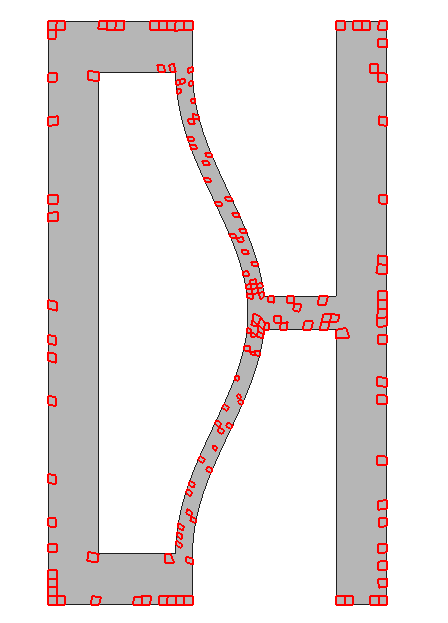
\includegraphics[width=\textwidth]{FIGS/p146.png}
        \caption{Equilibrium and PK1 output: $146$ points in $136$ elements.}
    \end{subfigure}
    \hspace{0.04\textwidth}
    \begin{subfigure}{0.38\textwidth}
        \centering
        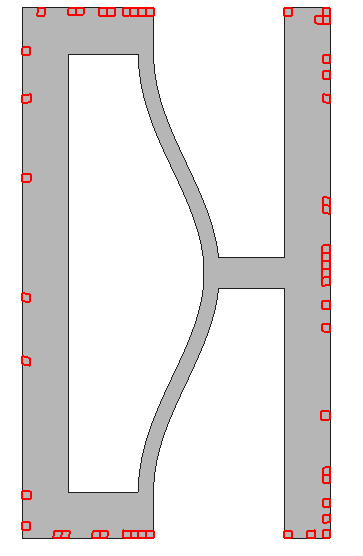
\includegraphics[width=\textwidth]{FIGS/p54.png}
        \caption{PK1 output only: $54$ points in $48$ elements.}
    \end{subfigure}
    \caption{Selected Gauss points for the fixed-weight manifold ECM. Compared
    with the standard HROM rule of Fig.~\ref{fig:elems1}, which required
    $1340$ points, the reduction is substantial. The decrease is mainly due to
    the fact that the tangent space of the nonlinear manifold has only
    $\rD=2$ directions, instead of the $\rROM=52$ fixed linear directions of the
    standard ROM. When only the stress-output block is retained, the cubature
    rule must reproduce only the PK1 stress integrands, leading to an even
    smaller set of points.}
    \label{fig:manifold_ECM_points}
\end{figure}

The comparison with Fig.~\ref{fig:elems1} is instructive. In the standard HROM,
each training state contributes $\rROM+\nstress=56$ scalar integrand fields.
In the manifold HROM, the equilibrium part contributes only
$\rD=2$ tangent directions, so each state contributes $2+4=6$ fields when both
equilibrium and output are included. The stresses themselves are not made
simpler by the manifold construction; rather, the virtual strains used to test
the internal force live in a two-dimensional tangent space that moves along the
curved manifold. This strongly reduces the dimension of the internal-force
density space seen by ECM. If the equilibrium block is removed altogether, only
the four stress-output components remain, explaining the further decrease from
$146$ to $54$ points.

\MATLAB{
The equilibrium--output case is run from
\href{/home/joaquin/Desktop/CURRENT_TASKS/MATLAB_CODES/TESTING_PROBLEMS_FEHROM/115_PAPER_MAW_ECM/01_METATcellHOM_2var/Run_HOMOG_2p.m}{Run\_HOMOG\_2p.m}
with input file
\href{/home/joaquin/Desktop/CURRENT_TASKS/MATLAB_CODES/TESTING_PROBLEMS_FEHROM/115_PAPER_MAW_ECM/01_METATcellHOM_2var/DATAINPUTS/Data_M4_hyperSTD.m}{Data\_M4\_hyperSTD.m}.
The flags are
\texttt{DATAoffline.ECMforReactionForces = true} and
\texttt{DATAoffline.ECMforEquilibrium = true}. The Newton tolerances for the
manifold HROM solve are set to
\texttt{TOL\_FORCES\_REL = 1e-10},
\texttt{TOL\_DISPLAC\_ABS = 1e-10}, and
\texttt{NMAXiter = 100}.
}

\MATLAB{
Although the main text writes the homogenized PK1 stress through the volume
average, the implementation uses the equivalent reaction-based route. The
reaction-output operator is assembled in
\href{/home/joaquin/Desktop/CURRENT_TASKS/MATLAB_CODES/FE_HROM/LARGE_STRAINS/NonLinearManifolds/DetermineModeReactionsOUTPUT_glo.m}{DetermineModeReactionsOUTPUT\_glo.m},
which calls
\href{/home/joaquin/Desktop/CURRENT_TASKS/MATLAB_CODES/FE_HROM/LARGE_STRAINS/NonLinearManifolds/DetermineModeHomogViaREACT.m}{DetermineModeHomogViaREACT.m}.
When the equilibrium and reaction-output blocks are concatenated, the
reaction-output block is normalized by its Frobenius norm and rescaled with the
Frobenius norm of the equilibrium block before the SVD, in order to balance the
two contributions.
}

\MATLAB{
The integrand blocks are assembled in
\href{/home/joaquin/Desktop/CURRENT_TASKS/MATLAB_CODES/FE_HROM/LARGE_STRAINS/NonLinearManifolds/OFFLINE_STAGE_nonECM_2var.m}{OFFLINE\_STAGE\_nonECM\_2var.m}.
Only the subsampled snapshots retained as RBF centers are used; this is encoded
through \texttt{DATA\_interp.indices\_subsampling\_SNAPSHOTS}. For each retained
state, the code stores the equilibrium and output contributions together in a
single block of size $\ngp\times(\rD+\nstress)$, rather than storing
$\AforceD$ and $\AP$ as two separate global matrices. This organization is
immaterial for a fixed ECM rule, but it prepares the data layout used later by
the manifold-adaptive-weight ECM.
}


 \PROMPT{\input{Prompt_onlineMHROMfw_1}}
\subsubsection{Online assessment of the fixed-weight manifold HROM}
\label{subsubsec:online_assessment_fixed_manifold}
%\input{onlineMHROMfw_1}


As already noted, the fixed-weight manifold construction leads to two online strategies. In the
first one, the master coordinates are identified  directly with the prescribed
macroscopic input, $\qM\approx\muvec$,
and the homogenized stress is obtained
by direct evaluation of the decoder and of the output cubature rule., and the homogenized stress is obtained
by direct evaluation of the decoder and of the output cubature rule. No reduced
equilibrium problem is solved. For a new input $\muvec$, one sets
$\qM=\muvec$, evaluates\footnote{From an implementation viewpoint, the same
computational pipeline as in the nonlinear manifold solve is retained. The only
difference is that the tentative value of the master coordinates is prescribed
directly from the macroscopic input, rather than initialized from the previous
pseudo-time step and subsequently corrected through Newton iterations. The
iterative stage is then effectively bypassed by imposing convergence tolerances
that are satisfied immediately.} $\dred=\Decod(\qM)$, and uses the lifting
\eqref{eq:dvecreconstruction} only on the elements containing the selected
cubature points. More precisely, if $\Esel$ denotes the set of elements
containing the selected Gauss points, only the restrictions
\[
    \left.\dvec\right|_{\Esel}
    =
    \left.
    \left(
    \Alift\Decod(\qM)+\Umacro\muvec
    \right)
    \right|_{\Esel}
\]
are needed for the evaluation of the stresses entering the reduced
homogenized-stress formula \refeq{eq:PKmacro_manifold_fixed_rule}. Thus, the online evaluation is a direct functional
evaluation on the selected elements, without pseudo-time continuation and
without Newton iterations.

The second strategy keeps the projected manifold equilibrium equation
 ~\eqref{eq:manifold_fixed_ECM_equilibrium}. In this case, for each prescribed
$\muvec$, the two master coordinates are obtained by solving a nonlinear
system of size $\rD=2$. The residual is
\[
    \bm{R}_{\mathcal{D}}(\qM;\muvec)
    =
    \sum_{g\in\ZD}
    \PhiD(\qM)^T
    \rFE{g}(\qM;\muvec)
    \,\wDg{g}.
\]
Its Newton linearization leads to the tangent matrix (that is, the Jacobian of
the reduced nonlinear system with respect to the master coordinates), which
contains two distinct contributions. Applying the chain rule gives Applying the chain rule
gives
\begin{equation}
\label{eq:manifold_tangent_split}
    \KtanD(\qM;\muvec)
    =
    \KstdD(\qM;\muvec)
    +
    \KcurvD(\qM;\muvec),
\end{equation}
where the standard tangent contribution is
\begin{equation}
\label{eq:manifold_standard_tangent}
    \KstdD
    =
    \sum_{g\in\ZD}
    \PhiD(\qM)^T
    \KFE_g(\qM;\muvec)
    \PhiD(\qM)
    \,\wDg{g},
\end{equation}
with $\KFE_g$ denoting the constrained Gauss-point tangent associated with
$\rFE{g}$. The additional term is caused by the dependence of the tangent basis
$\PhiD(\qM)$ on the state. Componentwise,
\begin{equation}
\label{eq:manifold_curvature_tangent}
    \left(\KcurvD\right)_{ab}
    =
    \sum_{g\in\ZD}
    \left[
    \derpar{^2\Decod}{q_{M,a}\,\partial q_{M,b}}(\qM)
    \right]^T
    \rFE{g}(\qM;\muvec)
    \,\wDg{g},
    \qquad
    a,b=1,\ldots,\rD .
\end{equation}
This residual-weighted curvature term is absent in a linear ROM because
$\PhiD$ is then constant. It is also commonly neglected in Gauss--Newton-type
linearizations of nonlinear projection-based ROMs when the residual is assumed
small near convergence \cite{barnett2022quadratic,ares2026nonlinear}. In the
present implementation it is retained whenever the second derivative of the
decoder is available.

The comparison with the standard HROM is reported in
Table~\ref{tab:online_fixed_manifold}. The errors are averaged over the two
training trajectories, as in Table~\ref{tab:standard_HROM_accuracy}. In the
manifold cases, the displacement error is not a pure consistency check: the RBF
closure is trained only on the $\nM=1540$ retained centers, whereas the
reported errors are evaluated over the full set of snapshots.

\begin{table}[H]
\centering
\caption{Online accuracy of the fixed-weight manifold HROM compared with the
standard HROM. The manifold models use $\rD=2$ master coordinates and
$\rROM-\rD=50$ slave coordinates.}
\label{tab:online_fixed_manifold}
\begin{tabular}{lccccc}
\toprule
Model & Master coords. & Slave coords. & $\nECM$ & $\errdisp$ & $\errPK$ \\
\midrule
ROM, full Gauss rule & $52$ & $0$ & $5260$
& $2.52\times10^{-6}$ & $5.05\times10^{-5}$ \\
 HROM, ECM & $52$ & $0$ & $1340$
& $1.85\times10^{-5}$ & $7.13\times10^{-5}$ \\
M-HROM, equil. + PK1 & $2$ & $50$ & $146$
& $9.64\times10^{-5}$ & $8.81\times10^{-3}$ \\
M-HROM, PK1   & $2$ & $50$ & $54$
& $7.87\times10^{-5}$ & $2.98\times10^{-4}$ \\
\bottomrule
\end{tabular}
\end{table}

% The output-only strategy gives the best stress accuracy among the two manifold
% variants. This is consistent with the input-driven character of the present
% problem: once $\qM$ has been identified with $\muvec$, solving an additional
% projected equilibrium equation may move the state away from the prescribed
% input-driven manifold coordinates, while the output-only rule evaluates
% directly the stress functional associated with the decoded state. The reduction
% in cubature points is nevertheless substantial in both cases: from $1340$ in
% the standard HROM to $146$ when equilibrium and output are retained, and to
% $54$ when only the stress output is integrated.

The output-only strategy gives the best stress accuracy among the two manifold
variants. This is a direct consequence of the exceptionally small residual in
the least-squares identification
$\qM=\Tm\qrom\approx\muvec$, which in the present case is of the order of
$10^{-7}$ (as we saw in Section \ref{subsec:num_char_fixed_manifold}). In other words, the macroscopic input variables already provide an
extremely accurate parametrization of the solution manifold. Under these
circumstances, solving an additional projected equilibrium problem in the
latent space brings essentially no additional information and may even
introduce small deviations from the input-driven manifold representation.
Accordingly, the most accurate strategy is simply to evaluate directly the
decoder and the reduced stress functional from the prescribed input
coordinates, without solving any nonlinear system.

It should be emphasized that this situation is highly problem-dependent. The
present example corresponds to a static hyperelastic homogenization problem
without internal history variables, for which the displacement manifold is
almost entirely parametrized by the macroscopic loading variables. As will be
shown later for history-dependent constitutive behavior, such as damage models,
this direct identification $\qM\approx\muvec$ no longer holds, and solving the
projected equilibrium equations becomes unavoidable.

Naturally, the manifold approximation introduces an additional source of error
with respect to the standard HROM. This is reflected in the increase of the
relative homogenized-stress error from approximately $7\cdot10^{-5}$ in the
standard HROM to roughly $3\cdot10^{-4}$ in the output-only manifold
approximation. Nevertheless, this deterioration remains moderate: the loss is
approximately one order of magnitude in accuracy, while the reduction in online
complexity is dramatically larger. Indeed, the number of required Gauss-point
evaluations decreases from the original $\ngp=5260$ points to only $54$, that
is, almost a two-order-of-magnitude reduction. Moreover, this reduction is
achieved without solving any nonlinear equilibrium problem during the online
stage: the response is obtained directly by evaluating the decoder and the
reduced stress functional.

% The present fixed-weight manifold approximation already demonstrates that,
% once the latent coordinates are aligned with the physical input parameters,
% substantial reductions in integration complexity become possible without severe
% loss of accuracy. For this reason, the output-only $54$-point cubature rule
% will be adopted in the sequel as the reference model for the adaptive-weight
% strategy.


At the same time, the present results also reveal the remaining limitation of
the fixed-weight paradigm. Despite the dramatic reduction from $5260$ to $54$
integration points, the resulting cubature rule still requires a number of
points approximately $25$ times larger than the number of latent coordinates
($\rD=2$). This indicates that the complexity of the cubature rule does not scale directly
with the dimension of the latent manifold itself.   This disparity can be expected to become
more pronounced as the dimension of the input parameter space increases. The
adaptive ECM introduced next is motivated precisely by this observation: rather
than enforcing a single cubature rule over the entire manifold, the integration
weights are allowed to evolve with the position on the manifold.

\MATLAB{
The Newton strategy is implemented in
\href{/home/joaquin/Desktop/CURRENT_TASKS/MATLAB_CODES/FE_HROM/LARGE_STRAINS/NonLinearManifolds/NewtonRapshonStaticLarge_manifoldMD.m}{NewtonRapshonStaticLarge\_manifoldMD.m}.
The residual and tangent are assembled from
\href{/home/joaquin/Desktop/CURRENT_TASKS/MATLAB_CODES/FE_HROM/LARGE_STRAINS/ResidualFromDisplacementsVAR.m}{ResidualFromDisplacementsVAR.m}.
The additional curvature contribution corresponds to the code block in which
\texttt{tauNONder2\_q} is contracted with \texttt{VAR.RESID\_extend}; this is
the implementation counterpart of Eq.~\refeq{eq:manifold_curvature_tangent}.
The equilibrium--output run uses
\href{/home/joaquin/Desktop/CURRENT_TASKS/MATLAB_CODES/TESTING_PROBLEMS_FEHROM/115_PAPER_MAW_ECM/01_METATcellHOM_2var/DATAINPUTS/Data_M4_hyperSTD.m}{Data\_M4\_hyperSTD.m},
whereas the output-only evaluation uses
\href{/home/joaquin/Desktop/CURRENT_TASKS/MATLAB_CODES/TESTING_PROBLEMS_FEHROM/115_PAPER_MAW_ECM/01_METATcellHOM_2var/DATAINPUTS/Data_M3_hyperSTD.m}{Data\_M3\_hyperSTD.m}.
}
\section{Manifold-adaptive weights ECM}
\label{sec:MAW_ECM}

\PROMPT{\input{ChangingChat_03}}

\PROMPT{\input{Prompt_MAWECM_1}}

\PROMPT{\input{Prompt_MAWECM_2}}

%\input{MAWECM_2}

\PROMPT{\input{Prompt_MAWECM_3}}

%\input{MAWECM_3}

\subsection{Motivation}
\label{sec:motivation_MAW_ECM}
The fixed-weight manifold HROM developed in the previous section already
achieves a substantial reduction of the integration cost. In particular, the
output-only formulation reduces the cubature rule to only \(54\) Gauss points,
while preserving an accurate approximation of the homogenized stresses.
Nevertheless, this result also reveals an important limitation of the fixed
cubature paradigm. Although the nonlinear manifold is parametrized here by only
\(\rD=2\) latent coordinates, the number of integration points remains
significantly larger than the intrinsic dimension of the manifold.

This observation is not accidental. The nonlinear manifold ROM recognizes that
the solution snapshots evolve on a curved low-dimensional manifold embedded in
the high-dimensional displacement space (i.e., $\dred \approx \Decod(\qM)$) . However, the cubature rule introduced
in Eqs.~\eqref{eq:manifold_fixed_ECM_equilibrium}--%
\eqref{eq:PKmacro_manifold_fixed_rule} does not exploit this geometric
structure locally. The same set of points \(\ZD\) and the same weights
\(\wDg{g}\) are used for all positions on the manifold, independently of the
current latent coordinate \(\qM\).



The origin of this limitation becomes clearer when examining the construction
of the ECM basis. For each sampled manifold state
\(({\qM}_j,\muvec_j)\), the corresponding equilibrium and stress-output
contributions are assembled through the block matrix introduced in
Eq.~\eqref{eq:aDP_single_state}. Each sampled state therefore contributes $\nDP:=\rD+\nstress$
scalar Gauss-point fields. In the present example, $\nDP = 2 + 4 = 6$
The global matrix used to construct the fixed cubature rule is then obtained by
concatenating all these local blocks over the sampled manifold, as expressed in
Eq.~\eqref{eq:manifold_fixed_ECM_training_matrix}.

This concatenation is the algebraic manifestation of a global integration
strategy. The cubature weights are required to satisfy, approximately, one
single set of linear equality constraints associated with the union of all
sampled integrand configurations over the manifold. In other words, although
the integrands evolve continuously with \(\qM\), the cubature operator itself
remains fixed.

The modification proposed in this section can be stated directly at the level
of the reduced integration rule. Instead of using the fixed weights
\(\wDg{g}\) appearing in
Eqs.~\eqref{eq:manifold_fixed_ECM_equilibrium}--%
\eqref{eq:PKmacro_manifold_fixed_rule}, we seek a reduced rule of the form
\begin{equation}
\label{eq:MAW_ECM_equilibrium_intro}
    \sum_{g\in\Zomega}
    \rDec{g}(\qM;\muvec)\,\omegag{g}(\qM)
    =
    \bm{0},
\end{equation}
for the manifold-projected equilibrium equations, and
\begin{equation}
\label{eq:MAW_ECM_PK_intro}
    \PKmacro
    \approx
    \frac{1}{|\Omega_0|}
    \sum_{g\in\Zomega}
    \PKone_g(\qM;\muvec)\,\omegag{g}(\qM)
\end{equation}
for the homogenized stress output. The set \(\Zomega\) is common to all
sampled manifold states and contains
\[
    \nomega := |\Zomega|
\]
integration points. What changes from one point of the manifold to another is
not the support, but the value of the weights.

Thus, each retained Gauss point \(g\in\Zomega\) is assigned a scalar field over
the latent space,
\[
    \omegag{g}:\mathbb{R}^{\rD}\rightarrow\mathbb{R}_{+},
    \qquad
    \qM\mapsto \omegag{g}(\qM).
\]
Equivalently, the cubature rule is described by the manifold-dependent vector
\[
    \omegavecq
    =
    \left[
    \omegag{g_1}(\qM),
    \ldots,
    \omegag{g_{\nomega}}(\qM)
    \right]^T,
    \qquad
    \Zomega=\{g_1,\ldots,g_{\nomega}\}.
\]
This is the sense in which the method is called a
manifold-adaptive weights ECM, or MAW--ECM: the integration points remain fixed
after the offline stage, whereas the associated ECM weights adapt to the
position on the nonlinear manifold.

The above problem conceals several challenging tasks from the optimization
point of view, namely:
\begin{enumerate}

 \item \label{item:MAW_sparsity} The final number of integration points (\(\nomega\)) should be as small
as possible.

\item \label{item:MAW_equa} The reduced cubature rule must reproduce, up to a prescribed tolerance,
the linear equality constraints associated with the manifold-projected
equilibrium equations~\refeq{eq:MAW_ECM_equilibrium_intro} and/or the output of interest (homogenized stress in this case, Eq.~\ref{eq:MAW_ECM_PK_intro}). In practice, each sampled
manifold state contributes \(\nDP=\rD+\nstress\) scalar integration
conditions, and the adaptive weights must satisfy all these local exactness
conditions with an user-prescribed accuracy throughout the sampled latent domain.

\item \label{item:positive}  The \(\nomega\) weights must remain nonnegative throughout the sampled
latent domain, while preserving the exact total volume, i.e.,
\(\sum_{g\in\Zomega}\omegag{g}(\qM)=|\Omega_0|\).

\item \label{item:smooth}   Finally, each scalar field \(\omegag{g}(\qM)\) should vary as smoothly
as possible over the manifold. Indeed, the adaptive weights will ultimately be
represented through a regression procedure over the latent domain (for instance
using RBF interpolation or neural networks), starting from weight values
computed at discrete sampled manifold states. Strong local oscillations or
abrupt changes between neighboring states would therefore deteriorate both the
regression accuracy of the weight fields and the robustness of the online stage
when iterative solvers are required to solve the reduced equilibrium equations.

\end{enumerate}


The rationale behind adaptive cubature weights is perhaps best understood on a
simple analytical example, where the mechanism can be examined explicitly. Consider the family of monomials
\[
    f_q(x)=x^q,
    \qquad
    x\in[0,1],
    \qquad
    q=0,1,\ldots,m .
\]
The exact integrals are
\[
    \int_0^1 f_q(x)\,dx
    =
    \frac{1}{q+1}.
\]
If one seeks a fixed integration rule capable of reproducing exactly all these
integrals simultaneously,
\[
    \int_0^1 f_q(x)\,dx
    =
    \sum_{g=1}^{n_{\mathrm{int}}}
    f_q(x_g)\,\omega_g,
    \qquad
    q=0,1,\ldots,m ,
\]
then the number of integration points must increase with the number of
monomials (as it happens in Gauss quadrature). However, if the weights are allowed to depend on the parameter \(q\), the whole
family can be integrated exactly using a single integration point located at
\(x=1\), i.e., \(\nomega=1\),
\[
    \int_0^1 f_q(x)\,dx
    =
    \omega(q)\,f_q(1),
    \qquad
    \omega(q)=\frac{1}{q+1}.
\]
Thus, instead of increasing the number of integration points in order to
capture the whole family with one fixed rule, the complexity is transferred to
a smooth parameter-dependent weight field.


%
%
% The same philosophy is adopted here. Rather than constructing a fully local
% cubature rule with a different support for each manifold point, the proposed
% MAW--ECM strategy retains a common support \(\ZMAW\) and transfers part of the
% complexity to a smooth manifold-dependent weight field. In this sense, the
% method occupies an intermediate position between a fully global fixed cubature
% rule and a fully local adaptive integration strategy.


\PROMPT{\input{Prompt_MAWECM_4}}

%  \input{LinearConstraints_1}

\PROMPT{\input{Prompt_MAWECM_5}}

\subsection{Initialization and local integration constraints}
\label{sec:MAW_local_constraints}
%\input{LinearConstraints_2}
%\input{LinearConstraints_3}
%\input{LinearConstraints_4}
The requirements \ref{item:MAW_sparsity}--\ref{item:smooth} will be formulated
in the sequel as a constrained optimization problem. Before doing so, however,
it is convenient to discuss the equality constraints entering the formulation
and the accuracy with which they are required to be satisfied. Firstly, we anticipate that the proposed construction follows an iterative
pruning strategy initialized from the fixed-weight ECM rule obtained from
Problem~\eqref{eq:ECM_problem_manifold_fixed}, whose sparse solution is \(\wD\in\mathbb{R}^{\ngp}\) and its support $  \ZD:=\operatorname{supp}(\wD)
    \subset\{1,\ldots,\ngp\}$.    Accordingly, the support associated with the adaptive cubature rule will be
sought within $\ZD$, i.e.,
\[
    \Zomega \subseteq \ZD .
\]
Let $\wDZ\in\mathbb{R}^{|\ZD|}$ denote the restriction of the sparse ECM weights \(\wD\) to
\(\ZD\). For subsequent developments, and in order to keep the optimization
formulation as general as possible, we introduce the notation
\[
    \omegaInit := \wDZ,
    \qquad
    \mInit := |\ZD| .
\]
where $|\ZD|$ denotes the cardinality of $\ZD$. Thus, \(\omegaInit\in\mathbb{R}^{\mInit}\) represents the initial vector of
candidate weights, while \(\mInit\) denotes the initial number of candidate
integration points prior to the adaptive pruning process.

The fact that the fixed ECM rule provides the reference integration rule for
  MAW--ECM algorithm   has important implications on the way
the integration conditions associated with
Eqs.~\eqref{eq:MAW_ECM_equilibrium_intro}--%
\eqref{eq:MAW_ECM_PK_intro} are interpreted.    As discussed in
Section~\ref{subsec:fixed_weight_manifold_hrom}, the state-wise equilibrium
and output blocks \(\aDP({\qM}_j)\), \(j=1,\ldots,\nM\), are first collected
over the sampled manifold and compressed through a truncated SVD. The left
singular vectors retained in \(\Ucub\) define the integrand subspace on which
the fixed ECM rule is exact. Thus, rather than requiring the reduced rule to reproduce the FE-quadrature
integrals of all columns of the original local block
\(\aDP({\qM}_j)\in\mathbb{R}^{\ngp\times(\rD+\nstress)}\), we require exact
reproduction only for their projection onto the retained local integrand
subspace. To this end, we define
\begin{equation}
\label{eq:MAW_projected_local_block}
    \uDP({\qM}_j)
    :=
    \Ucub\Ucub^T\aDP({\qM}_j)
    \in
    \mathbb{R}^{\ngp\times\ncond},
    \qquad
    j=1,\ldots,\nM .
\end{equation}
The fixed ECM rule then satisfies
\begin{equation}
\label{eq:MAW_fixed_rule_local_exactness}
    \uDP({\qM}_j)^T\wD
    =
    \uDP({\qM}_j)^T\wFE,
    \qquad
    j=1,\ldots,\nM .
\end{equation}
These equalities define the local integration conditions inherited by the
adaptive construction.


The projected blocks \(\uDP({\qM}_j)\) are not the only constraints entering
the adaptive construction. Requirement~\ref{item:positive} in
Section~\ref{sec:motivation_MAW_ECM} already imposes exact reproduction of the
total volume, which may be regarded as a manifold-independent invariant of the
cubature rule. More generally, one may wish to enforce additional invariant
integration properties uniformly over the sampled manifold, such as exact reproduction of low-order geometric moments (e.g. inertia moments) or of reference integrands associated with the
 linear regime.   Such constraints are not
attached to any particular manifold state, but are instead required to hold for
every adaptive cubature rule.  We collect these state-independent exactness constraints in a block
\[
    \Uinv\in\mathbb{R}^{\ngp\times\ninv}.
\]
(at minimum, \(\Uinv\) contains the constant integrand
\(\onevec\in\mathbb{R}^{\ngp}\), i.e., an all-ones vector)

For each sampled point \({\qM}_j\), the full-grid local constraint basis is
obtained by combining the invariant block with the projected local integrand
content,
\[
    \Ubarj{j}
    :=
    \operatorname{orth}
    \left(
    \left[
    \Uinv,\,
    \uDP({\qM}_j)
    \right]
    \right)
    \in
    \mathbb{R}^{\ngp\times\ncond},
    \qquad
    j=1,\ldots,\nM .
\]
The orthogonalization removes redundant conditions between the invariant block
and the local projected fields.
The adaptive unknowns are initialized on the fixed ECM support \(\ZD\).
Therefore, the constraint basis used in the adaptive problem is the restriction
of \(\Ubarj{j}\) to the rows indexed by \(\ZD\):
\[
    \Uj{j}
    :=
    \Ubarj{j}\big|_{\ZD}
    \in
    \mathbb{R}^{\mInit\times\ncond}.
\]
The corresponding local right-hand side inherited from the reference fixed rule
is
\[
    \bj{j}
    :=
    \Uj{j}^{T}\omegaInit
    \in
    \mathbb{R}^{\ncond}.
\]
Thus, at the sampled manifold state \({\qM}_j\), the adaptive weights must
satisfy
\begin{equation}
\label{eq:constraintsLOCAL}
    \Uj{j}^{T}\omegaj{j}
    =
    \bj{j},
    \qquad
    j=1,\ldots,\nM .
\end{equation}
Here \(\omegaj{j}\in\mathbb{R}^{\mInit}\) denotes the adaptive weight vector
associated with \({\qM}_j\), still expressed on the initial candidate support
\(\ZD\). The subsequent pruning process will progressively eliminate entries of
these vectors while preserving the same local equality constraints.


\PROMPT{\input{ChangingChat_04}}

 \PROMPT{\input{Prompt_Spars_1}}

\subsection{Sparsification problem}
\label{sec:sparsification_problem}
 %\input{Spars_1}
 \PROMPT{\input{Prompt_Spars_2}}
The local exactness conditions in~\eqref{eq:constraintsLOCAL} define, at each
sampled manifold state \(\qMj{j}\), a feasible set of adaptive cubature
weights. The unknowns of the problem are therefore not a single cubature vector,
but the collection
\[
\left\{
\omegaj{1},
\omegaj{2},
\ldots,
\omegaj{\nM}
\right\},
\]
where each
\[
\omegaj{j}\in\mathbb{R}^{\mInit}
\]
contains the cubature weights associated with the sampled latent state
\(\qMj{j}\), expressed on the initial candidate support \(\ZD\).

Equivalently, the adaptive weights may be gathered into the matrix
\begin{equation}
\label{eq:3333333}
\Wad
=
\begin{bmatrix}
| & | &  & | \\
\omegaj{1} & \omegaj{2} & \cdots & \omegaj{\nM} \\
| & | &  & |
\end{bmatrix}
\in
\mathbb{R}^{\mInit\times\nM},
\end{equation}
whose columns correspond to the sampled manifold states and whose rows define
discrete weight fields over the latent manifold.

The central objective of MAW--ECM is to identify the smallest possible common
support capable of satisfying all local constraints
simultaneously. Since the weights are constrained to remain nonnegative, the
vector
\[
\sum_{j=1}^{\nM}\omegaj{j}
\]
has a nonzero entry at position \(i\) if and only if the \(i\)-th candidate
integration point receives a nonzero weight for at least one sampled manifold
state. Therefore,
the cardinality of the union of all local supports may be measured through the
\(\ell_0\) pseudo-norm
\begin{equation}
\label{eq:support1}
\left\|
\sum_{j=1}^{\nM}
\omegaj{j}
\right\|_0 .
\end{equation}
This support-union interpretation closely parallels the formulation advocated
by the authors in~\cite{bravo2024subspace} in the context of subspace-adaptive
weights ECM (SAW--ECM), which may be regarded as the subspace counterpart of
the present manifold-adaptive construction. The main difference is that the
discrete subspace index is here replaced by a sampled nonlinear manifold of
latent states. Furthermore, unlike a finite collection of essentially
independent subspaces, neighboring points on the latent manifold are expected
to induce related local cubature rules, whose associated adaptive weights
should evolve in a sufficiently smooth and coherent manner across the manifold. Consequently, besides
promoting a sparse common support, it is also natural to penalize excessively
irregular variations of the adaptive weights over the latent manifold, in the
sense discussed in Item~\ref{item:smooth} of Section \ref{sec:motivation_MAW_ECM}.

Based on the above considerations, we propose the following
manifold-adaptive sparsification problem:
\begin{equation}
\begin{aligned}
\min_{\omegaj{1},\ldots,\omegaj{\nM}}
\quad &
\left\|
\sum_{j=1}^{\nM}
\omegaj{j}
\right\|_0
+
 \Reg(\Wad)
\\
\text{subject to}
\quad &
\Uj{j}^{T}\omegaj{j}
=
\bj{j},
\qquad
j=1,\ldots,\nM,
\\
&
\omegaj{j}\ge0,
\qquad
j=1,\ldots,\nM .
\end{aligned}
\label{eq:MAW_global_l0}
\end{equation}

The first term in the objective function promotes a sparse common support shared
across the sampled manifold states ( that is, it seeks to minimize the total
number of integration points), whereas the regularization
functional \(\Reg(\Wad)\) penalizes highly irregular variations of the adaptive
weights over the latent manifold. To put it differently, \(\Reg(\Wad)\) measures the distortion of the adaptive
weight fields relative to the initial fixed-weight configuration, for which all
sampled manifold states share the same cubature weights and thus  \(\Reg(\Wad)\) vanishes. The parameter \(\alpha\ge0\) controls the
strength of this regularization.  It should be noted that,  at this juncture of the discussion, \(\Reg(\Wad)\)
is introduced only in abstract form.  Specific choices associated with the
constructive pruning strategy will be discussed later.

\subsection{Pruning strategy}

\subsubsection{Overview}

\PROMPT{\input{Prompt_pruning1}}

%\input{Pruning_1}

The formulation of Problem~\eqref{eq:MAW_global_l0} is valuable at the conceptual level because it
provides an explicit mathematical formulation of the manifold-adaptive
sparsification objective underlying MAW--ECM.  Nevertheless, much like the fixed-weight formulation
in~\eqref{eq:ECM_problem_manifold_fixed}, the problem is not amenable to direct
solution in practice because it belongs to the class of
\(\ell_0\)-minimization problems, which are well known to be NP-hard
\cite{natarajan1995sparse}. In other words, the difficulty stems from the
combinatorial nature of the \(\ell_0\)-term in the objective function.




Practical approaches for \(\ell_0\)-minimization problems typically rely either on suboptimal greedy
procedures or on suitable convex relaxations, most commonly obtained by
replacing the \(\ell_0\)-objective with an \(\ell_1\)-based surrogate
promoting sparsity. For instance,  the latter strategy is   the philosophy underlying the Empirical Quadrature Method, EQM, introduced by Patera and co-workers
\cite{yano2019discontinuous,yano2019lp} to solve Problem   \eqref{eq:ECM_problem_manifold_fixed} in alternative way to that of those based on nonnegative least-squares concept, as in the ECM  and the ECSW.


\PROMPT{\input{Prompt_pruning2}}

%\input{Pruning_2}
%\input{Pruning_3}
The \(\ell_1\)-based convexification route was previously explored by the
authors in~\cite{bravo2024subspace} in the context of the aforementioned
SAW--ECM (the sparsification problem  in SAW--ECM is structurally
analogous to Problem~\eqref{eq:MAW_global_l0}, but without the
manifold-regularization term). The main
conclusion drawn in~\cite{bravo2024subspace} (and that applies for the problem at hand) is that the \(\ell_1\)-based
convexification route is not viable in practice. The reason is twofold. Firstly, the LP formulation requires stacking all
adaptive weight vectors into a single global optimization variable (in the
present notation, this amounts to vectorizing the matrix \(\Wad\) introduced
in Eq.~\eqref{eq:3333333}, leading to a variable of dimension \(\mInit\nM\)). In
doing so, the formulation loses sight of the fundamentally local nature of the
cubature constraints associated with each sampled manifold state, while the
computational cost rapidly becomes prohibitive as \(\nM\) grows. Secondly,
even in relatively small problems for which the LP problem remains tractable,
the numerical experiments reported in~\cite{bravo2024subspace} showed that the
resulting supports were systematically larger than those obtained with the
final greedy SAW--ECM strategy.


Accordingly, the present work does not pursue this \(\ell_1\)-based route, but
instead adopts a greedy iterative strategy that avoids treating the entire
global optimization variable simultaneously. The underlying idea is inspired by
the \emph{pruning} strategies employed in the derivation of generalized
quadrature rules \cite{bremer2010nonlinear,xiao2010numerical}, where the goal
is likewise to identify the smallest possible set of integration points,
including both their positions and weights. This philosophy was adopted by the
authors in~\cite{hernandez2024cecm} to derive a
continuous\footnote{The qualifier continuous refers to the fact that the
positions of the cubature points are treated as continuous design variables,
rather than as members of a discrete candidate set subject to selection.}
version of ECM.

% The analogy with the present MAW--ECM setting is the following. In both cases,
% the starting point is an already feasible cubature rule possessing more points
% than strictly necessary. Sparsification is then achieved progressively by
% eliminating points that contribute the least to the satisfaction of the
% integration and positiveness constraints, while continuously readjusting the remaining weights
% so that the constraints remain satisfied. In this sense, both approaches view
% sparsification not as a global combinatorial search over all admissible
% supports, but rather as a sequential pruning process that progressively drives
% as many weights as possible to zero.

The analogy with the present MAW--ECM setting is the following. In both cases,
the starting point is an already feasible cubature rule possessing more points
than strictly necessary. Sparsification is then achieved progressively by
eliminating points that contribute the least to the satisfaction of the
integration and positivity constraints, while continuously readjusting the
remaining weights so that the constraints remain satisfied. In this sense,
both approaches view sparsification not as a global combinatorial search over
all admissible supports, but rather as a sequential pruning process in which
integration points are removed one at a time from a common support while the
remaining weights are redistributed to preserve local exactness conditions.

The essential difference lies in the nature of the design variables. In
generalized quadrature rules~\cite{bremer2010nonlinear,xiao2010numerical} and
in CECM~\cite{hernandez2024cecm}, both the positions and the weights of the
cubature points are allowed to evolve continuously during the pruning process.
In the present MAW--ECM setting, by contrast, the candidate points are fixed
Gauss points inherited from the underlying finite element discretization, and
only the manifold-dependent weights are modified. Moreover, in the present problem, the adaptive weights cannot evolve
independently from one manifold state to another, but must vary in a
sufficiently smooth and coherent manner over the latent manifold; enforcing
such smoothness is precisely the role of the regularization term.

\PROMPT{\input{ChangingChat_05}}

\subsubsection{Pruning algorithm}
\PROMPT{\input{Prompt_pruning3}}



\section{Concluding remarks}

\PROMPT{\input{Prompt_conclusions}}







 \bibliographystyle{plain}
\bibliography{Bibliography}

\end{document}
